%pour la mise en page
\documentclass[a4paper,10pt]{report}
\usepackage[utf8]{inputenc}
\usepackage[Conny]{fncychap}
%Sonny Lenny Glenn Conny Rejne et Bjarne

%pour les maths
\usepackage{graphicx}
\usepackage{amsmath}
\usepackage{indentfirst}
\usepackage{amssymb}

%pour les figures
\usepackage{float}

%pour les algorithmes
\usepackage{algorithm}
\usepackage{algorithmic}
%francisation des algorithmes
\renewcommand{\algorithmicrequire} {\textbf{\textsc{Initialisation}}}
\renewcommand{\algorithmicensure}  {\textbf{\textsc{Sorties:}}}
\renewcommand{\algorithmicand}      {\textbf{et}}
\renewcommand{\algorithmicwhile}   {\textbf{Tant que}}
\renewcommand{\algorithmicdo}      {\textbf{faire}}
\renewcommand{\algorithmicendwhile}{\textbf{fin tant que}}
\renewcommand{\algorithmicend}     {\textbf{fin}}
\renewcommand{\algorithmicif}      {\textbf{Si}}
\renewcommand{\algorithmicendif}   {\textbf{fin si}}
\renewcommand{\algorithmicelse}    {\textbf{Sinon}}
\renewcommand{\algorithmicthen}    {\textbf{alors}}
\renewcommand{\algorithmicfor}     {\textbf{Pour}}
\renewcommand{\algorithmicforall}  {\textbf{Pour tout}}
\renewcommand{\algorithmicendfor}  {\textbf{fin pour}}
\renewcommand{\algorithmicloop}    {\textbf{Boucler}}
\renewcommand{\algorithmicendloop} {\textbf{fin boucle}}
\renewcommand{\algorithmicrepeat}  {\textbf{Répéter}}
\renewcommand{\algorithmicuntil}   {\textbf{Jusqu'à}}

\usepackage{color}
\definecolor{gray}{rgb}{0.5, 0.5, 0.5}
\definecolor{lightgray}{rgb}{0.96, 0.96, 0.96}
\definecolor{orange}{rgb}{1.0, 0.5, 0.0}
\definecolor{blue}{rgb}{0.0, 0.0, 1.0}
\definecolor{red}{rgb}{0.8, 0.0, 0.0}

%pour les programmes
\usepackage{listings}
	\lstset{
		language=scilab,
		basicstyle=\small,
		keywordstyle=\bf \color{orange},
		identifierstyle=\color{blue},
		commentstyle=\color[gray]{0.5},
		stringstyle=\color{red},
		showstringspaces=false,
		numbers=left,
		numberstyle=\tiny \bf \color{gray},
		numbersep=10pt,
		numberfirstline=true,
		backgroundcolor=\color{lightgray},
}

\usepackage[top=3cm, bottom=3cm, left=3cm, right=3cm]{geometry}

\renewcommand{\chaptername}{Chapitre}
\renewcommand{\contentsname}{Table des matières}
\renewcommand{\listfigurename}{Table des Figures}
\renewcommand{\listtablename}{Table des Codes}
\renewcommand{\tablename}{Code}

\usepackage{eso-pic}
	\newcommand\BackgroundPic{%
		\put(0,0){
			\parbox[b][\paperheight]{\paperwidth}{%
			\vfill
			\centering
			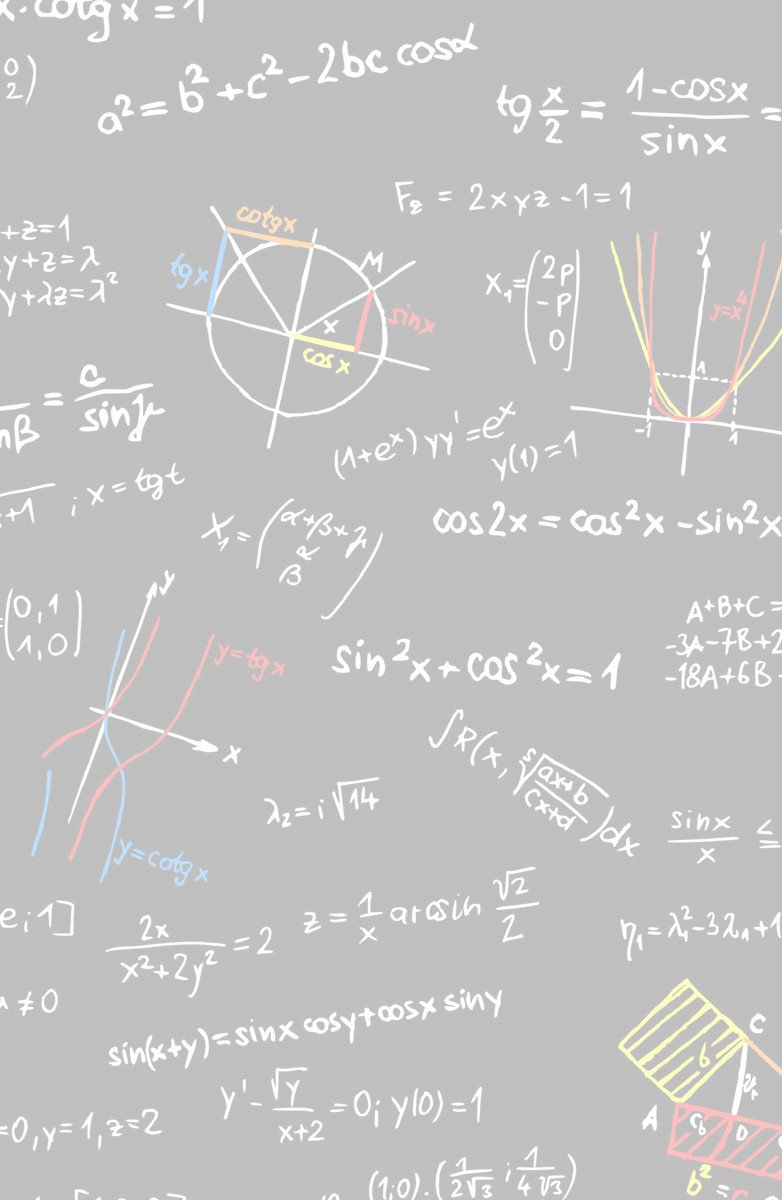
\includegraphics[width=\paperwidth,height=\paperheight]{mathtimes.png}%
			\vfill
		}}}

\usepackage{fancyhdr}
\pagestyle{fancy}
\renewcommand\headrulewidth{1pt}
\fancyhead[L]{Cahier d'intégration MT94}
\fancyhead[R]{\leftmark}
\renewcommand\footrulewidth{1pt}
\fancyfoot[L]{UTC}
\fancyfoot[C]{\thepage}
\fancyfoot[R]{Marlow Justine}

\makeatletter
\let\ps@plain=\ps@fancy
\makeatother

\begin{document}
\AddToShipoutPicture*{\BackgroundPic}
\title{Cahier d'intégration MT94}
\author{Marlow Justine}
\date{}
\maketitle

\addcontentsline{toc}{chapter}{Table des matières}
\tableofcontents
\newpage
\addcontentsline{toc}{chapter}{Table des figures}
\listoffigures
\newpage
\addcontentsline{toc}{chapter}{Table des codes}
\listoftables

\newpage
\addcontentsline{toc}{chapter}{Résumé}
\chapter*{Résumé}
\markboth{RESUME}{}
Blabla résumé, MT94

\chapter{Problèmes non linéaires I}

\section{Introduction}
\indent Les problèmes non linéaires constituent un ensemble de problèmes mathématiques qui sont, pour la plupart, insolubles de manière analytique. Ces problèmes peuvent en effet se ramener à la recherche des solutions de $f(x)=0$. Or la recherche de racines devient problématique lorsque le degré du polynôme $f$ augmente, impossible de déterminer des solutions analytiquement pour un degré supérieur ou égal à 4. Il existe donc des méthodes numériques afin d'approcher ces solutions. Nous allons étudier quelques une de ces méthodes au sein de ce chapitre.\\ \\
\indent Les trois premières méthodes étudiées, à savoir \textit{la dichotomie}, \textit{la méthode des points fixes} et \textit{la méthode de Newton}, concernent les problèmes à une inconnue : $f : \mathbb{R} \longrightarrow \mathbb{R}$. Nous verrons également l'application de \textit{la méthode de la sécante}, qui se trouve être une méthode dérivée de \textit{la méthode de Newton}. La dernière méthode étudiée, qui est également \textit{la méthode de Newton}, permet de traiter des problèmes à $n$ ($n>1$) inconnues : $f : \mathbb{R}^n \longrightarrow \mathbb{R}^n$.\\ \\
\indent Pour chacune de ces méthodes, nous étudierons tout d'abord leur aspect théorique avant de les appliquer dans \textit{Scilab}. Cette application suivra toujours la même démarche :
\begin{itemize}
\item Résoudre le problème par exécution du code
\item Tracer la courbe de l'erreur en fonction de l'itération avec la commande : \begin{verbatim} --> plot(erreur,'o')
\end{verbatim}
\item Tracer la courbe de régression linéaire avec la commande : \begin{verbatim}
--> plot(log(erreur(1:k-1))',log(erreur(2:k))')
\end{verbatim} et connaître son coefficient directeur avec la commande : \begin{verbatim}
--> reglin(log(erreur(1:k-1))',log(erreur(2:k))')
\end{verbatim}
\end{itemize}

\newpage
\section{La dichotomie ou bissection}
\subsubsection{Théorie}
La dichotomie est une méthode de résolution numérique répandue et enseignée dés le lycée. Son principal avantage est qu'elle ne nécessite qu'une seule hypothèse : la continuité de $f$ sur un intervalle $I\subset \mathbb{R}$.\\
\indent La fonction $f : \mathbb{R} \longrightarrow \mathbb{R}$ est donc continue sur un intervalle $I$. On va par ailleurs supposer que l'on travaille sur un intervalle $[a,b]\subset I$ tel que $f(a)f(b)<0$. La continuité de $f$ permet d'appliquer le théorème des valeurs intermédiaires : il existe $x^{*}\in[a,b]$ tel que $f(x^{*})=0$.\\
\indent Le principe de l'algorithme est alors le suivant : on définit :\\ $(a_{n})_{,\ n \geq 0},\ (b_{n})_{,\ n \geq 0},\ a_{0}=a,\ b_{0}=0,\ (x_{n})_{, n \geq 0},\ x_{n} = \frac{a_{n}+b_{n}}{2}, a_{n+1}$ et $b_{n+1}$ par:

\begin{algorithm}
\begin{algorithmic}
\WHILE{$|f(x_n)|>\varepsilon$ ($\varepsilon$ désigne la précision recherchée)}
\IF{$f(a_{n})f(b_{n})>0$}
\STATE $a_{n+1}=x_{n}$
\ELSE
\STATE $b_{n+1}=x_{n}$
\ENDIF
\ENDWHILE
\end{algorithmic}
\end{algorithm}

\indent Pour juger de l'efficacité de cette méthode, on s'intéresse à la convergence de la suite. Par construction, on a $(b_{n} - a_{n})=(\frac{1}{2}){n}(b_{0} - a_{0})$.\\
Ainsi $|x_{n} - x^{*}|\leq\frac{1}{2}(b_{n} - a_{n})$ donc $|x_{n} - x^{*}|\leq\frac{1}{2}^{n+1}(b_{0} - a_{0})$.

\subsubsection{Application}
Pour cette application, on étudie $f : \mathbb{R} \longrightarrow \mathbb{R}$ définie telle que $f(x)=x^2-2$. On connaît évidemment la solution de cette équation, il s'agit de $\pm\sqrt{2}$. On choisit donc un intervalle $[a,b]$ qui encadre seulement une solution, $\sqrt{2}$, on prendra ici $[a,b]=[1,2]$. On implémente donc dans \textit{Scilab} le code \ref{dichotomie}.
\begin{table}[H]
\label{dichotomie}
\caption{Dichotomie}
\begin{tabular}{l}
\lstinputlisting[language=scilab]{dichotomie.sce}\\
\end{tabular}
\end{table}

On trace l'évolution de l'erreur en fonction de l'itération (figure \ref{graph_dicho}).
\begin{center}
\begin{figure}[H]
\caption{Erreur en fonction de l'itération}
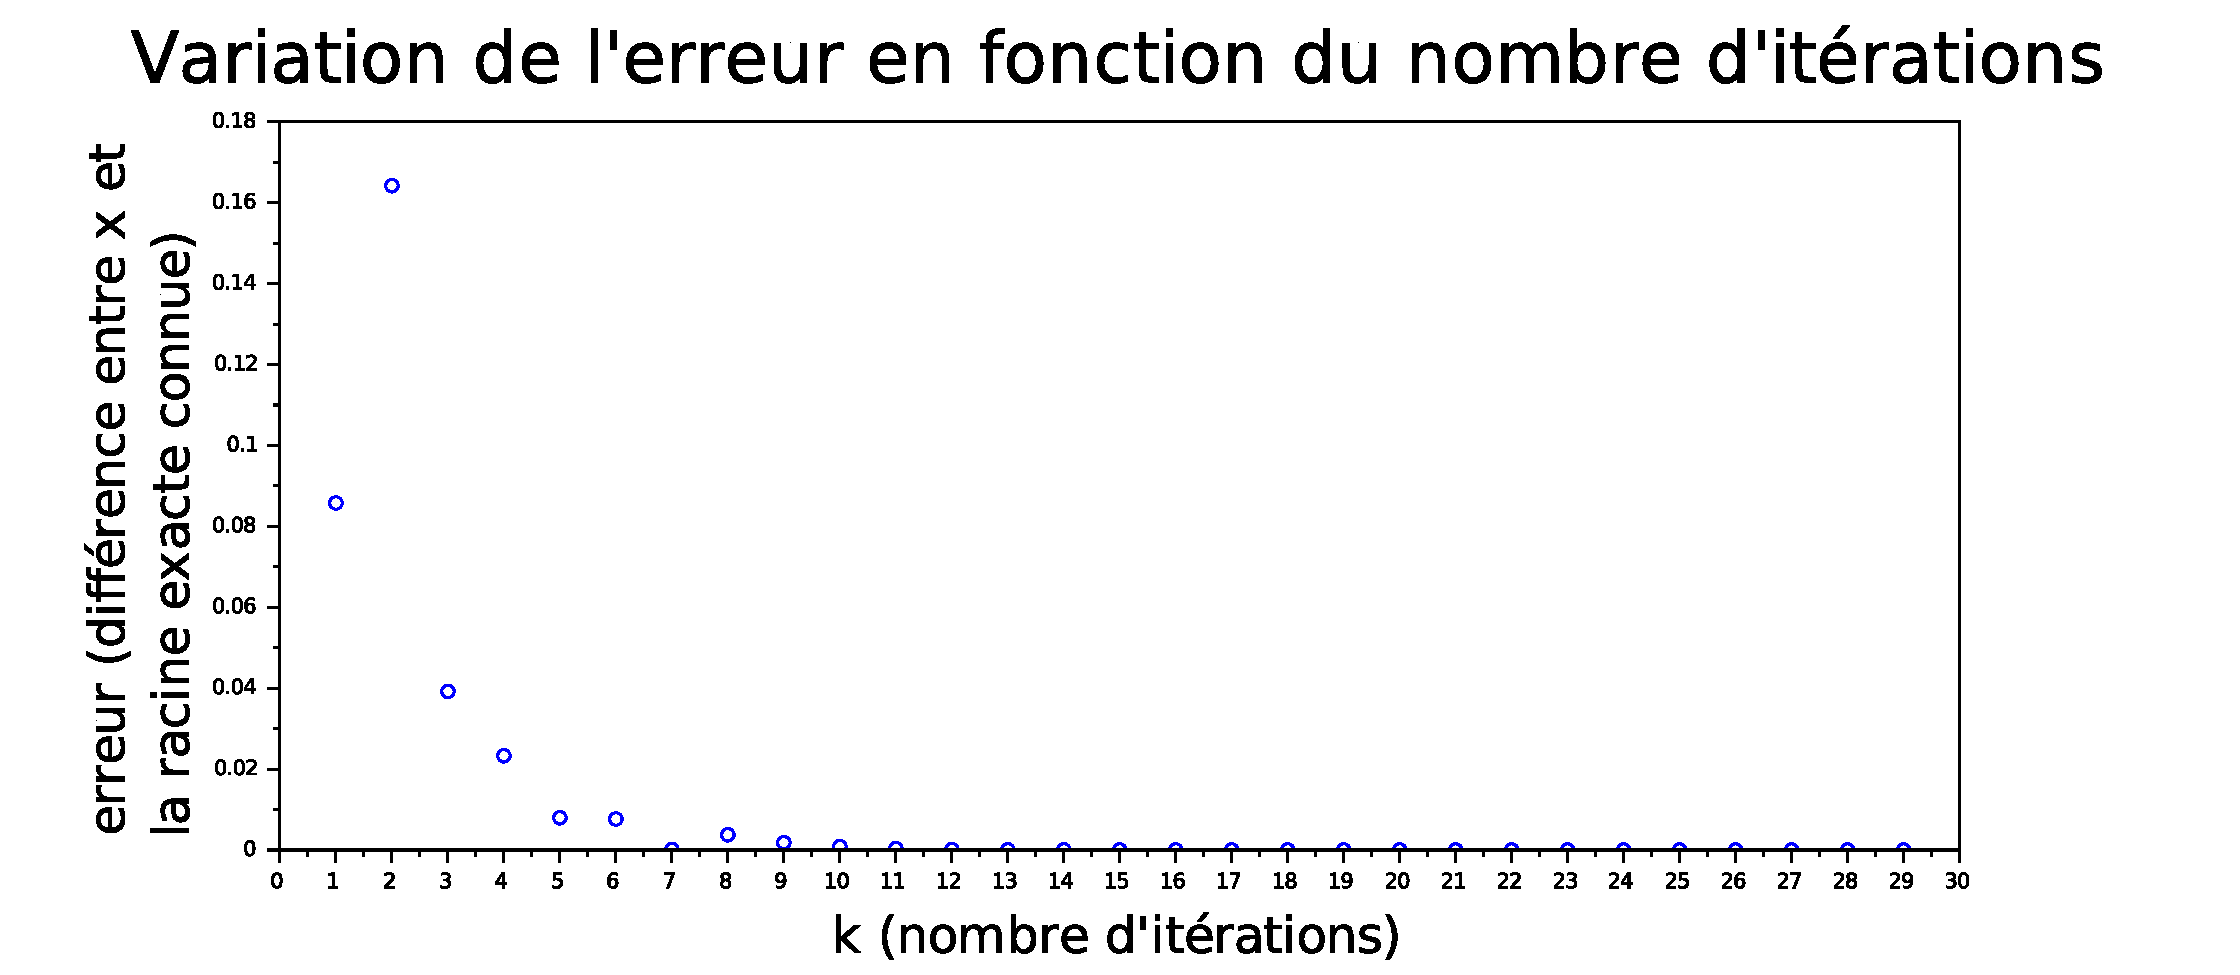
\includegraphics[width=\textwidth]{graphdicho.pdf}
\label{graph_dicho}
\end{figure}
\end{center}

Puis on s'intéresse à l'évolution de l'erreur relative (figure \ref{erreur_dicho}).
\begin{center}
\begin{figure}[H]
\caption{Diminution relative de l'erreur en fonction de l'itération}
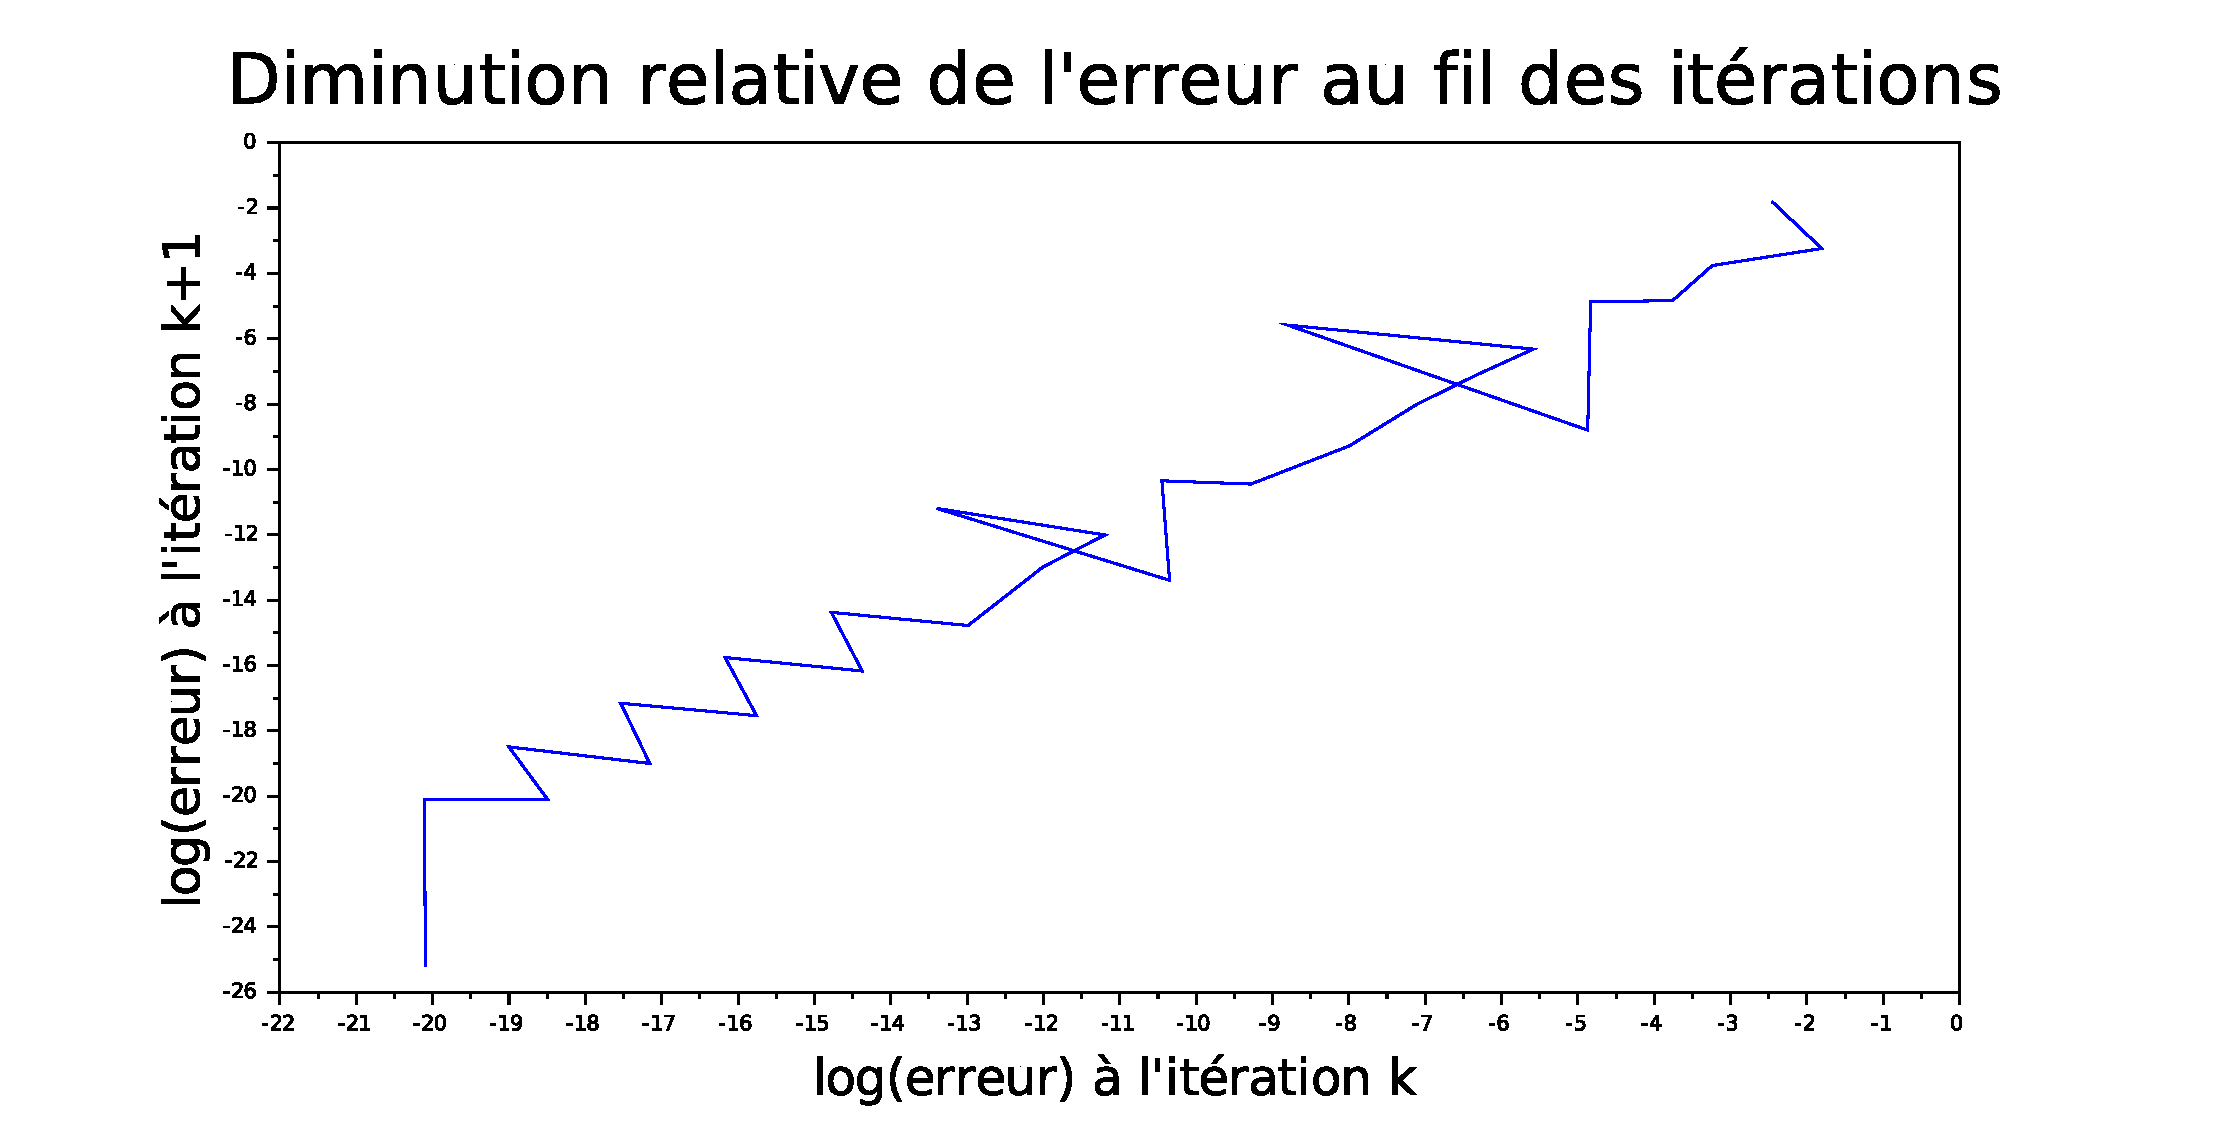
\includegraphics[width=\textwidth]{graphdicho_reg.pdf}
\label{erreur_dicho}
\end{figure}
\end{center}

La solution est donc approchée en 29 itérations. Une remarque toute particulière pour la dichotomie : l'erreur n'est pas réduit de manière uniforme au fil des itérations (comme le montre la figure \ref{erreur_dicho}). Si on linéarise cette courbe (figure \ref{erreur_dicho}) grâce à \textit{Scilab}, on obtient un coefficient proche de 1 (environ 1,0188), il s'agit effectivement d'une convergence linéaire, ou d'ordre 1.

\newpage
\section{La méthode de point fixe}
\subsubsection{Théorie}
Cette méthode, également répandue, nécessite toutefois plus d'hypothèses que la dichotomie, en effet il est nécessaire que $f$ soit une fonction dérivable.\\
\indent L'idée de la méthode est de rechercher une fonction $g : \mathbb{R} \longrightarrow \mathbb{R}$ telle que $f(x)=0 \Leftrightarrow g(x)=x$. Cette fonction $g$ (supposée dérivable) admet ainsi un point fixe, notons le $x^*$ tel que $|g'(x^*)|<1$. Alors, en appliquant le théorème des accroissements finis, il existe $[a,b]$ tel que $x^*\in[a,b]$ et la suite :\\
$
\left\lbrace
\begin{array}{l}
x_0\in[a,b]\\
x_{n+1}=g(x_n), n\geq0
\end{array}\right.
$ converge vers $x^*$ (la démonstration est admise ici, détaillée en MT90).\\ \\
\indent Comme avec la dichotomie, s'intéresser à la convergence de la suite nous indique sur l'efficacité de la méthode. Si $g'(x^*)\neq0$ alors $\frac{|x_{n+1}-x^*|}{|x_{n}-x^*|}<k$ avec $0<k<1$. \\
\noindent Par récurrence, $|x_{n+1}-x^*|<k^n|x_{0}-x^*|$.

\subsubsection{Application}
A nouveau, on étudie $f : \mathbb{R} \longrightarrow \mathbb{R}$ définie telle que $f(x)=x^2-2$. Comme précédemment, on choisit l'intervalle $[a,b]=[1,2]$, et on choisit ici $x_0=\frac{3}{2}$ (on se place au milieu de l'intervalle d'étude). On implémente donc dans \textit{Scilab} le code \ref{code_pointfixe}.

\begin{table}[H]
\caption{Point fixe}
\begin{tabular}{l}
\lstinputlisting[language=scilab]{pointfixe.sce}
\label{code_pointfixe}
\end{tabular}
\end{table}

\newpage
On trace l'évolution de l'erreur en fonction de l'itération (figure \ref{graph_pointfixe}).
\begin{figure}[H]
\centering
\caption{Erreur en fonction de l'itération}
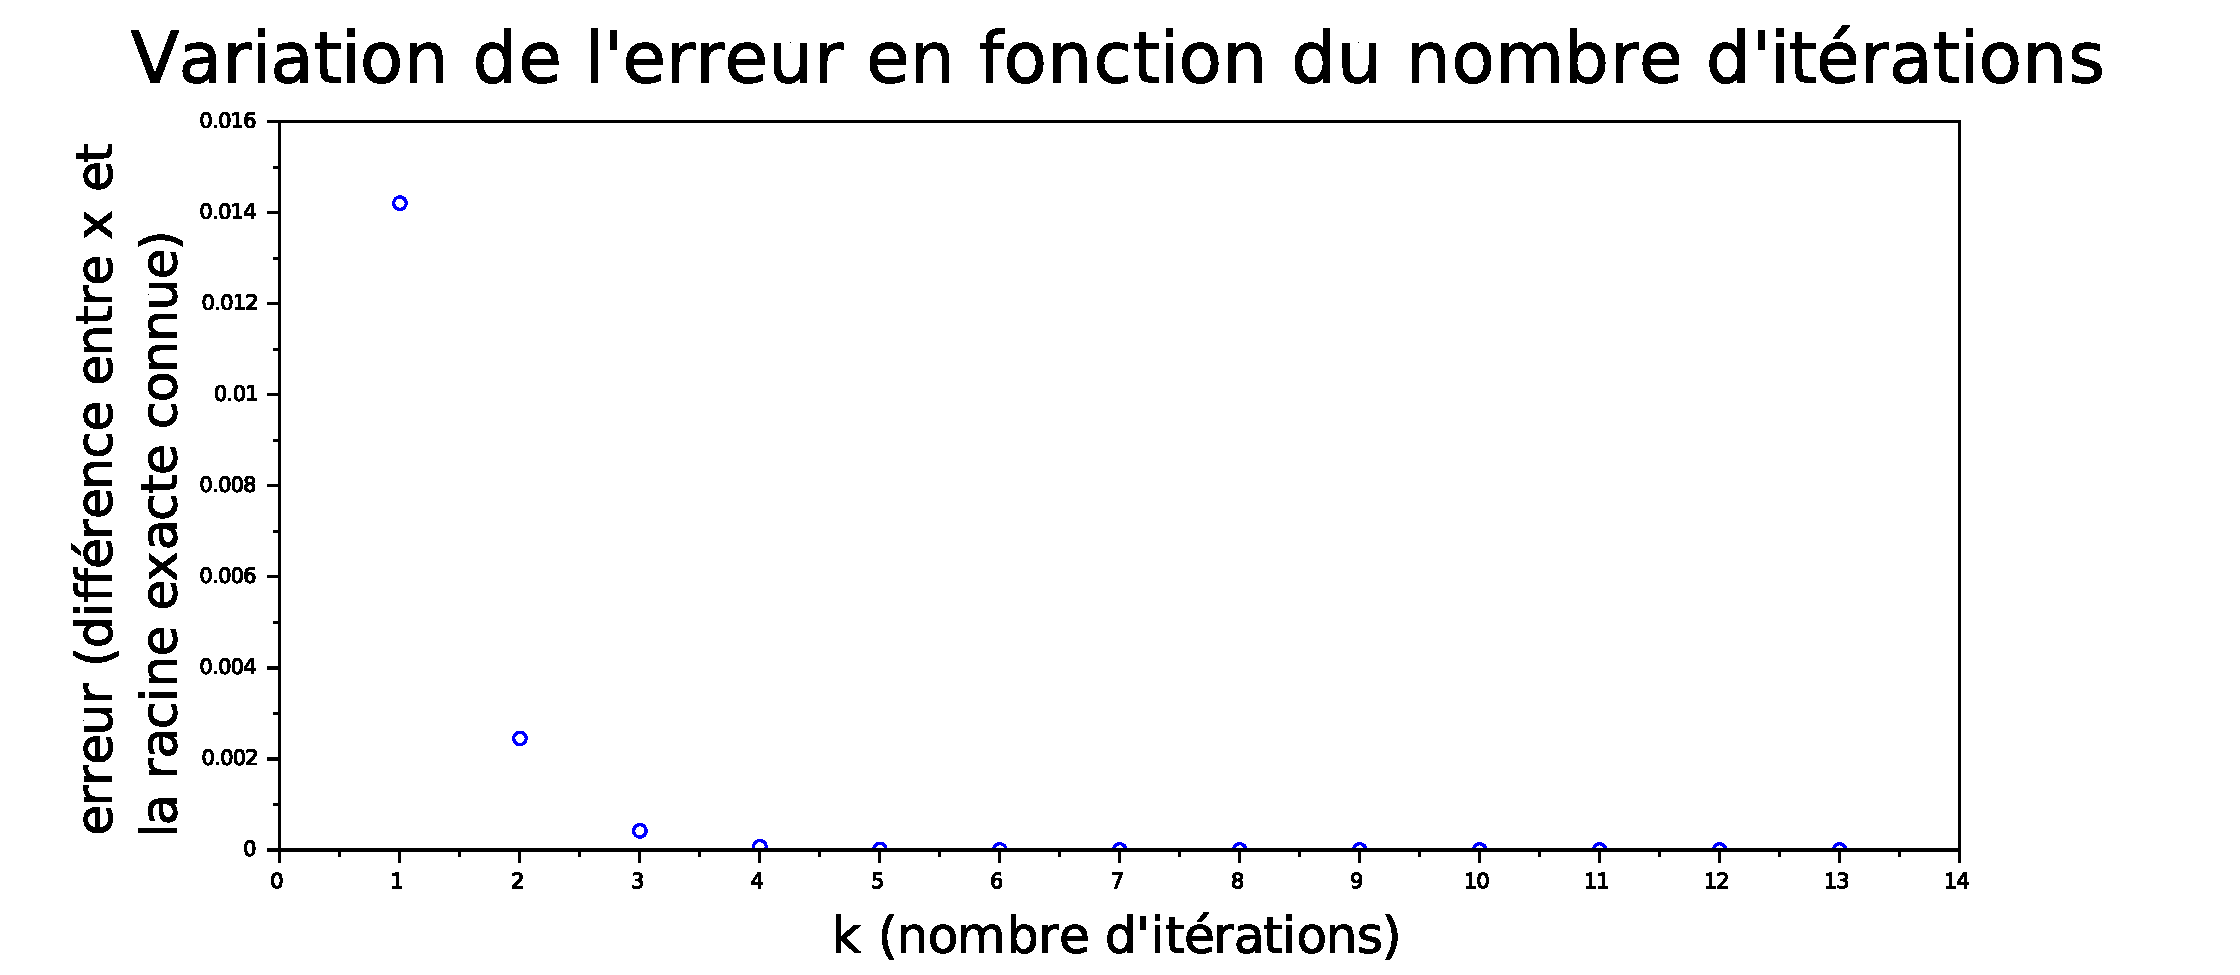
\includegraphics[width=\textwidth]{graphpointfixe.pdf}
\label{graph_pointfixe}
\end{figure}

Puis on s'intéresse à l'évolution de l'erreur relative (figure \ref{erreur_pointfixe}).
\begin{center}
\begin{figure}[H]
\caption{Diminution relative de l'erreur en fonction de l'itération}
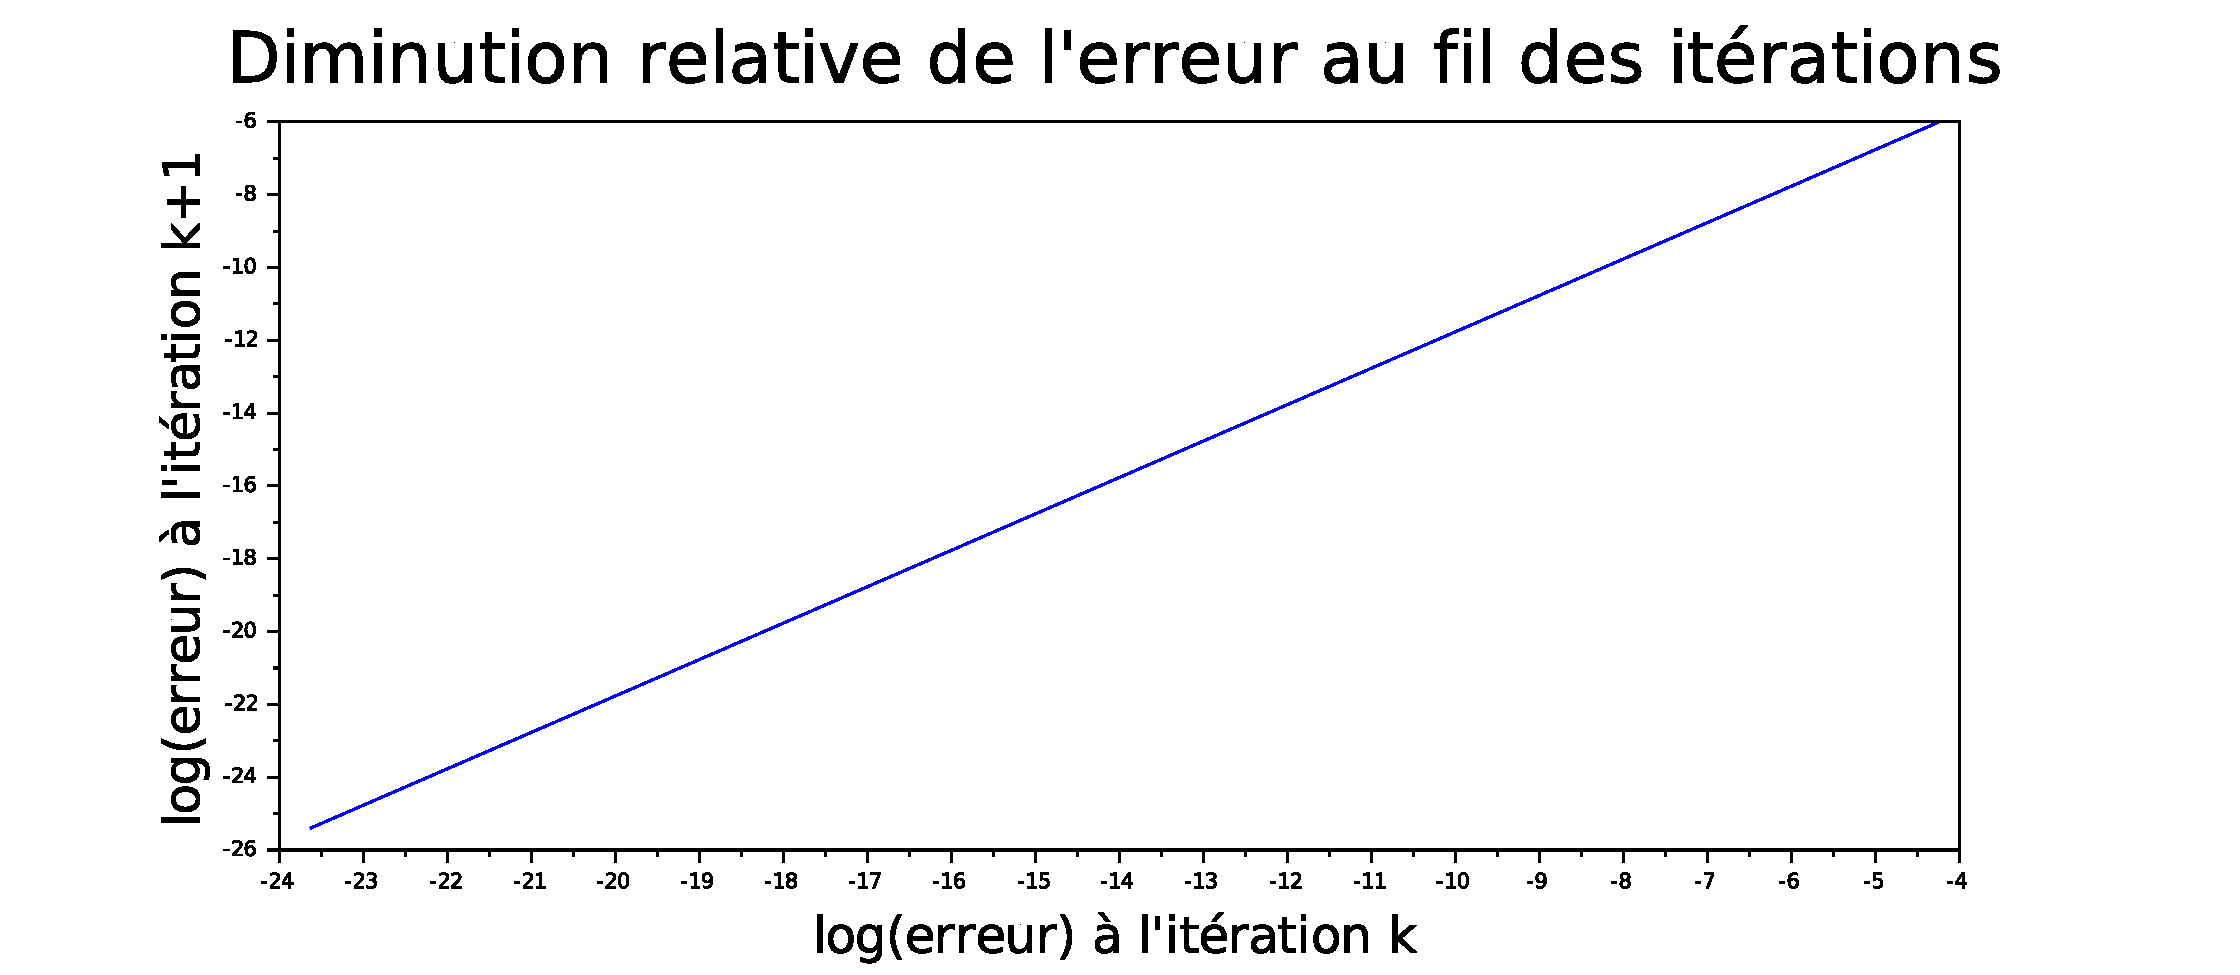
\includegraphics[width=\textwidth]{graphpointfixe_reg.pdf}
\label{erreur_pointfixe}
\end{figure}
\end{center}

La solution est donc approchée en 13 itérations. Si on linéarise cette courbe (figure \ref{erreur_pointfixe}) grâce à \textit{Scilab}, on obtient un coefficient très proche de 1 (environ 1,0001), effectivement, il s'agit à nouveau d'une convergence d'ordre 1.

\newpage
\section{La méthode de Newton appliquée à $n=1$}
\subsubsection{Théorie}
La méthode de Newton nécessite encore plus d'hypothèses que les deux méthodes que nous venons d'étudier. En effet, on suppose ici que la fonction $f$ est deux fois continûment dérivable. On écrit ensuite le développement de Taylor Lagrange sur $f$ : soit $x_{0}\in\mathbb{R}$, il existe $\theta\in]0,1[$,\\
$f(x_0+h)=f(x_0)+f'(x_0)h + \frac{h^2}{2}f''(x_0+\theta h)$\\
si on pose $x=x_0+h$, le développement devient :\\
$f(x)=f(x_0)+f'(x_0)(x-x_0) + \frac{{x-x_0}^2}{2}f''(x_0+\theta (x-x_0))$\\
On effectue l'approximation affine de $f(x)$ : $T_{x_0}(x)=f(x_0)+f'(x_0)(x-x_0)$\\
et on définit $x_1$ par $T_{x_0}(x_1)=0 \Leftrightarrow f(x_0)+f'(x_0)(x_1-x_0)=0$\\
si $f'(x_0)\neq0$ alors $x_1=x_0 - \frac{f(x_0)}{f'(x_0)}$.\\
Ainsi, graphiquement, la méthode de Newton consiste à tracer une droite tangente à $y=f(x)$ en $x_n$, $x_{n+1}$ est alors la racine de cette tangente.\\
\indent L'algorithme est donc le suivant : pour $x_0$ donné, et $\varepsilon$ la précision à atteindre,
\begin{algorithm}
\begin{algorithmic}
\WHILE{$|f(x_n)|>\varepsilon$}
\STATE $x_{n+1} =  x_{n}-\frac{f(x_n)}{f'(x_n)}$
\ENDWHILE
\end{algorithmic}
\end{algorithm}

\indent On peut remarquer que la méthode de Newton est une méthode de point fixe particulière.
En effet $x_{n+1}=x_n-\frac{f'(x_0)}{f'(x_0)} \Leftrightarrow x_{n+1}=g(x_n)$ avec $g(x)=x-\frac{f(x)}{f'(x)}$
Ainsi $g'(x)=1-\frac{f'(x)^2-f(x)f''(x)}{f'(x)^2}$, on émet l'hypothèse que $f'(x^*)\neq0$, donc $g'(x)=1-\frac{f'(x^*)^2}{f'(x^*)^2} = 0$, d'où $|g'(x^*)|<1$.\\
\indent On s'intéresse maintenant à la convergence de cette suite, toujours pour juger de l'efficacité de la méthode. Si on suppose que f est trois fois continûment dérivable, on a $x_{n+1}-x^*=g(x_n)-g(x^*)$, $g(x_n)=g(x^*)+(x_n-x^*)g'(x^*)+\frac{(x_n-x^*)^2}{2}g''(\xi)$ $\Rightarrow |x_{n+1}-x^*|\leq C|x_n-x^*|^2$ avec $C=\frac{1}{2}max|g''(\xi)|$.


\subsubsection{Application}
Encore une fois, on étudie $f : \mathbb{R} \longrightarrow \mathbb{R}$ définie telle que $f(x)=x^2-2$. Comme précédemment, on choisit l'intervalle $[a,b]=[1,2]$ et $x_0=\frac{3}{2}$.On implémente donc dans \textit{Scilab} le code \ref{code_newton}.

\begin{table}[H]
\caption{Newton (appliquée à $n=1$)}
\begin{tabular}{l}
\lstinputlisting[language=scilab]{newton.sce}
\label{code_newton}
\end{tabular}
\end{table}

On trace l'évolution de l'erreur en fonction de l'itération (figure \ref{graph_newton}).
\begin{figure}[H]
\centering
\caption{Erreur en fonction de l'itération}
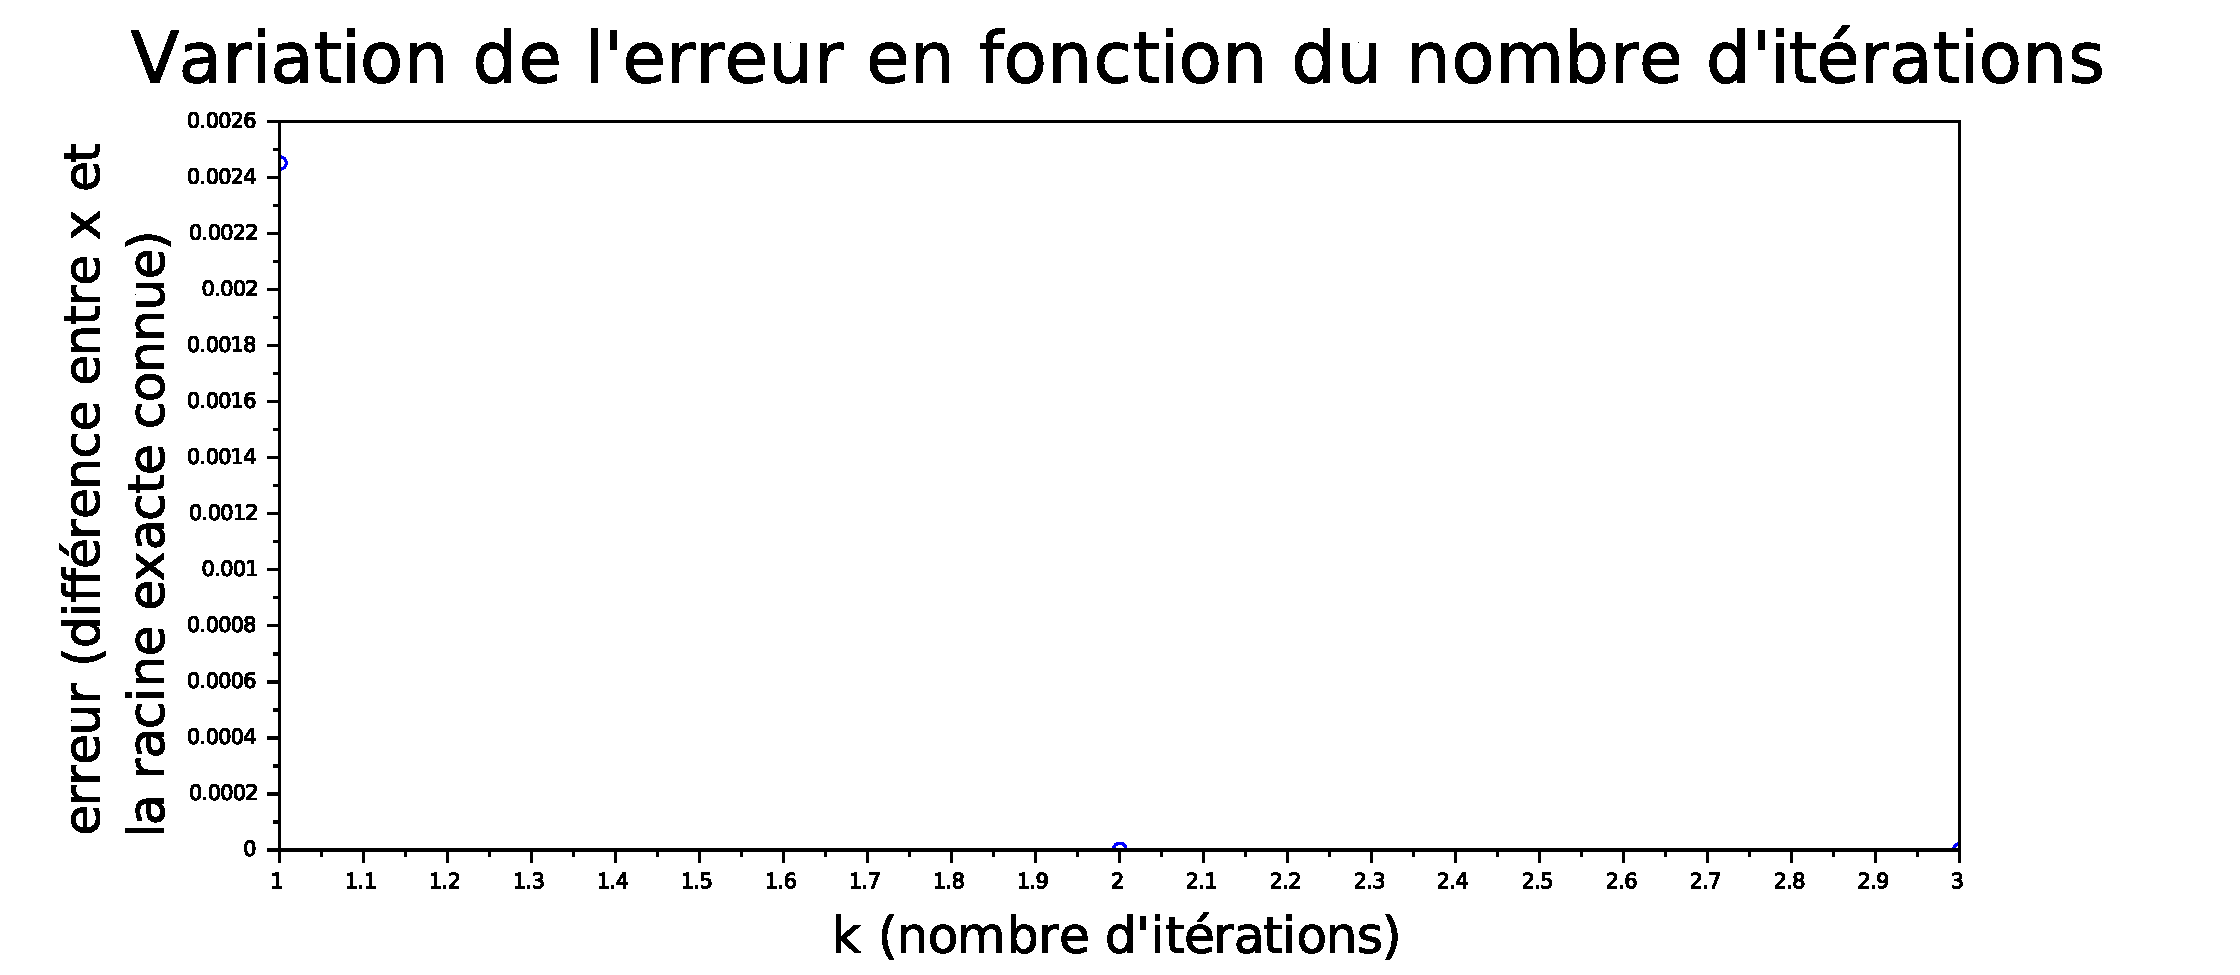
\includegraphics[width=\textwidth]{graphnewton.pdf}
\label{graph_newton}
\end{figure}

Puis on s'intéresse à l'évolution de l'erreur relative (figure \ref{erreur_newton}).
\begin{figure}[H]
\centering
\caption{Diminution relative de l'erreur en fonction de l'itération}
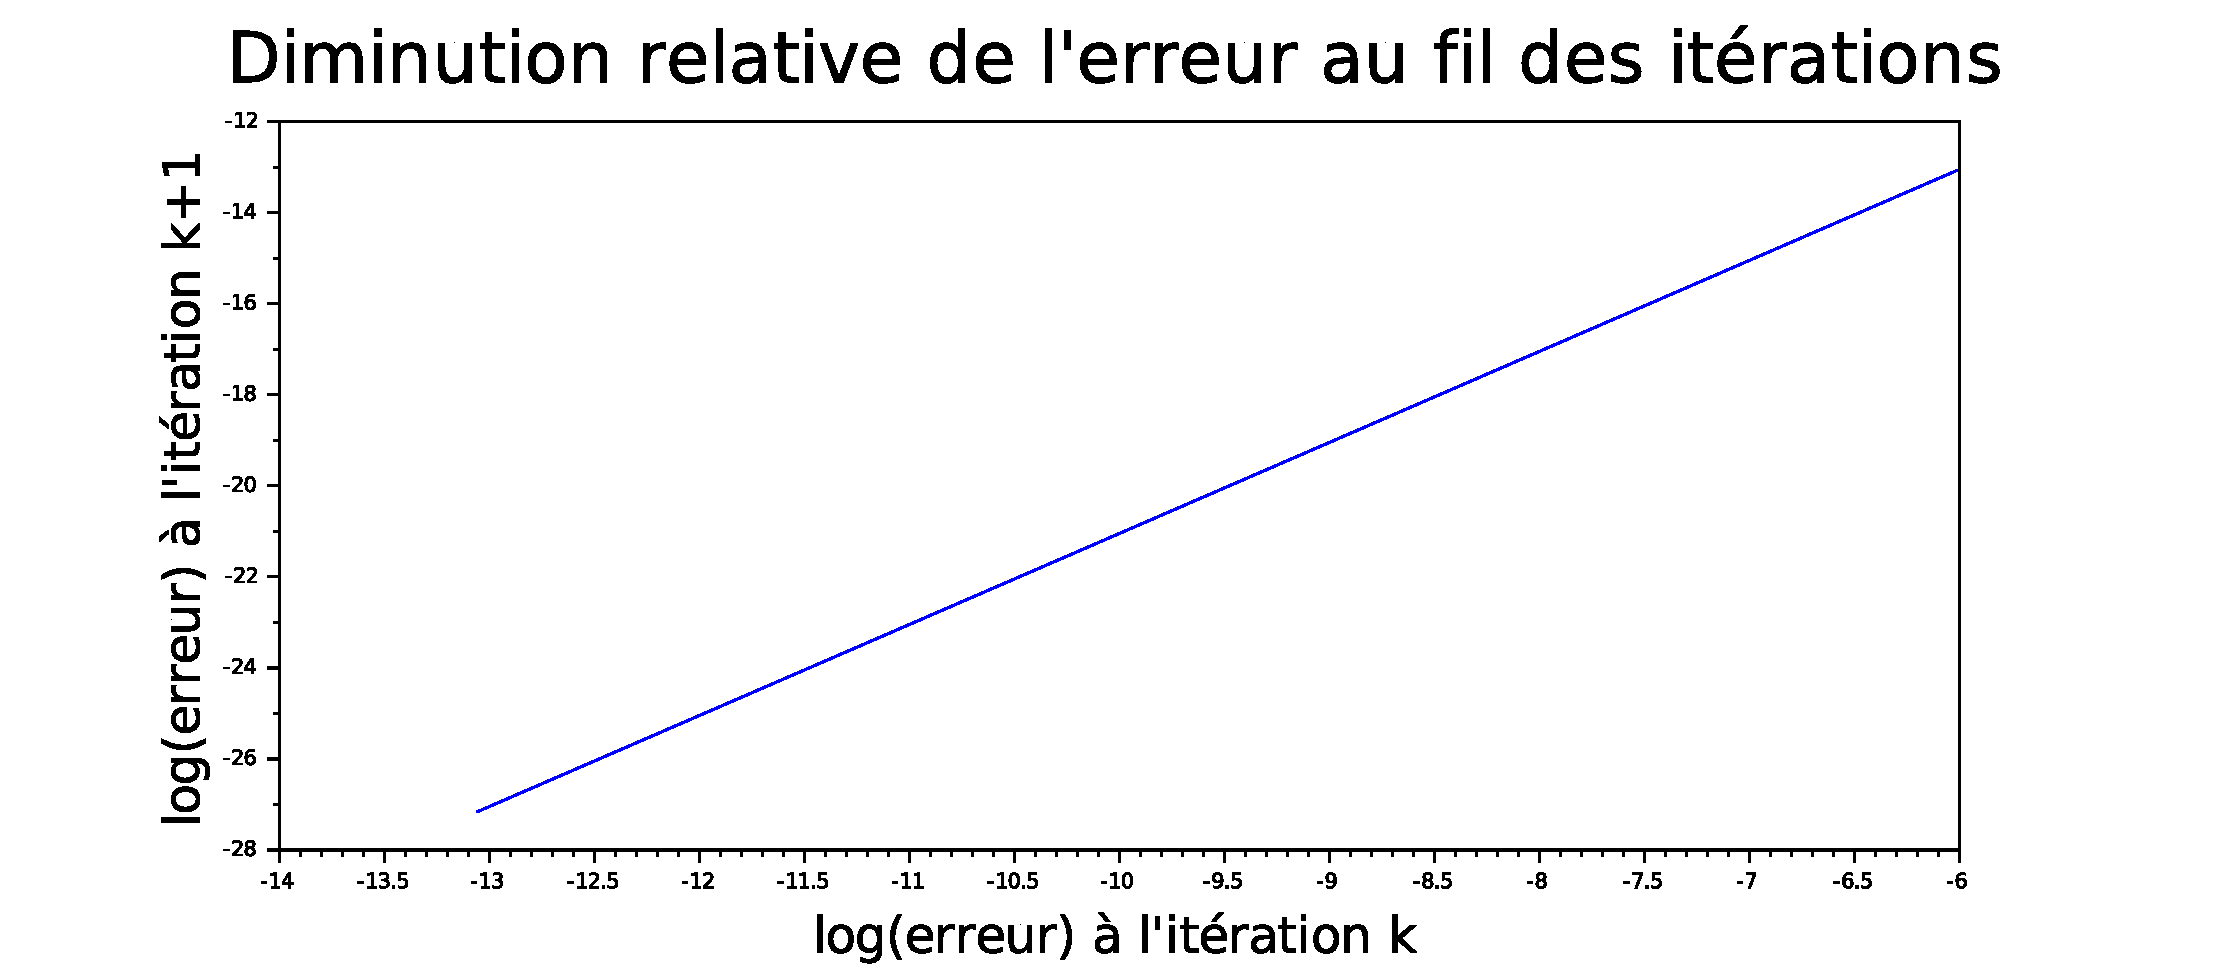
\includegraphics[width=\textwidth]{graphnewton_reg.pdf}
\label{erreur_newton}
\end{figure}

La solution est donc approchée en 3 itérations. Si on linéarise cette courbe (figure \ref{erreur_newton}) grâce à \textit{Scilab}, on obtient un coefficient très proche de 2 (environ 1,9998), il s'agit effectivement d'une convergence quadratique ou d'ordre 2.

\newpage
\section{La méthode de la sécante}
\subsubsection{Théorie}
Comme nous l'avons évoqué précedemment, la méthode de la sécante est directement dérivée de la méthode de Newton.
En effet, dans l'algorithme, on prenait $x_n+1=x_n-\frac{f(x_n}{f-(x_n)}$. Pour la méthode de la sécante, il suffit d'approcher $f'(x_n)$ par le taux d'accroissement, à savoir $\frac{f(x_n)-f(x_{n+1}}{x_n-x_{n+1}}$.\\ \\
L'algorithme devient donc, pour $x_0$ et $x_1$ donnés :
\begin{algorithm}
\begin{algorithmic}
\WHILE{$|f(x_n)|>\varepsilon$}
\STATE $x_{n+1} =  x_{n}-\frac{f(x_n)}{f(x_n)-f(x_{n+1})}(x_n-x_{n+1})$
\ENDWHILE
\end{algorithmic}
\end{algorithm}

\subsubsection{Application}
On étudie une dernière fois $f : \mathbb{R} \longrightarrow \mathbb{R}$ telle que $f(x)=x^2-2$. Comme précédemment, on choisit l'intervalle $[a,b]=[x_0,x_1]=[1,2]$. On implémente donc dans \textit{Scilab} le code \ref{code_secante}.

\begin{table}[H]
\caption{Sécante}
\label{code_secante}
\begin{tabular}{l}
\lstinputlisting[language=scilab]{secante.sce}\\
\end{tabular}
\end{table}

\begin{center}
\begin{figure}[H]
\caption{Erreur en fonction de l'itération}
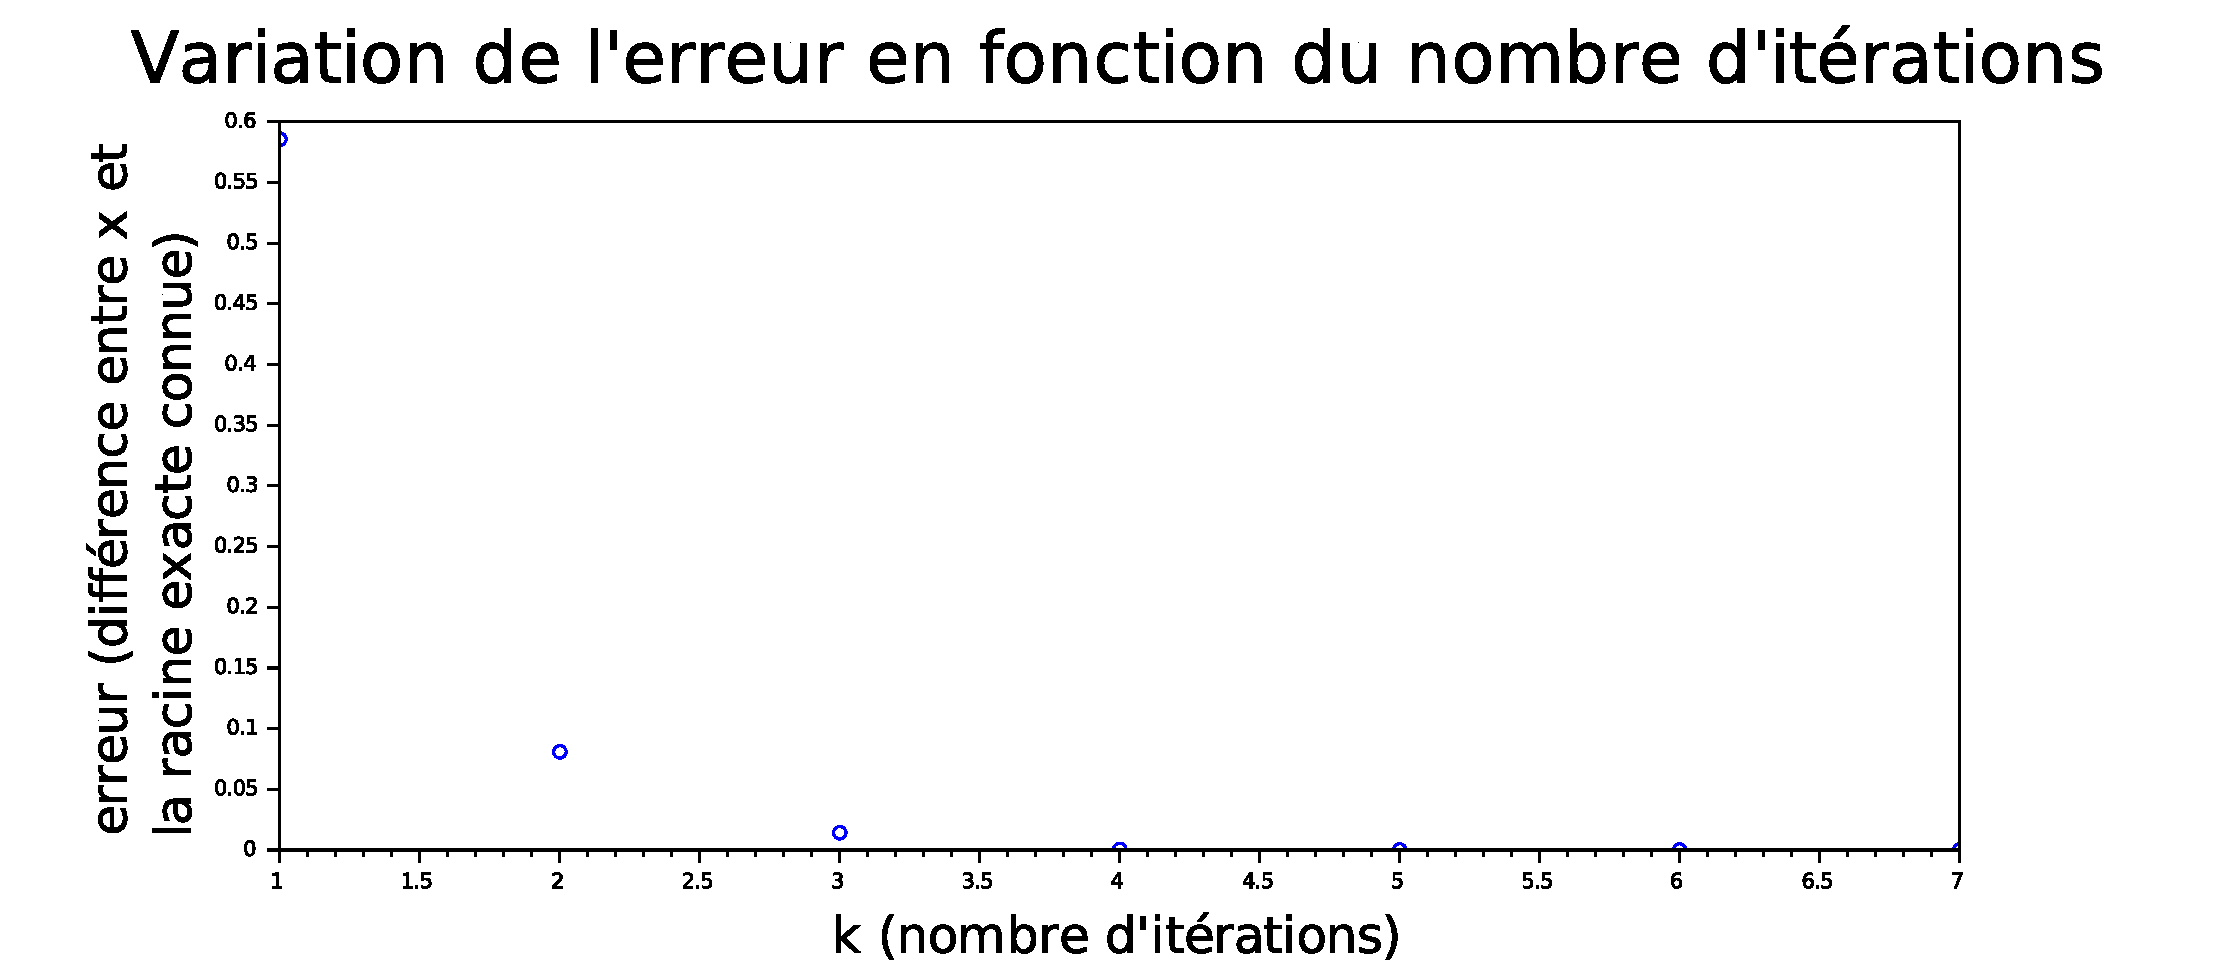
\includegraphics[width=\textwidth]{graphsecante.pdf}
\end{figure}

\begin{figure}[H]
\caption{Diminution relative de l'erreur en fonction de l'itération}
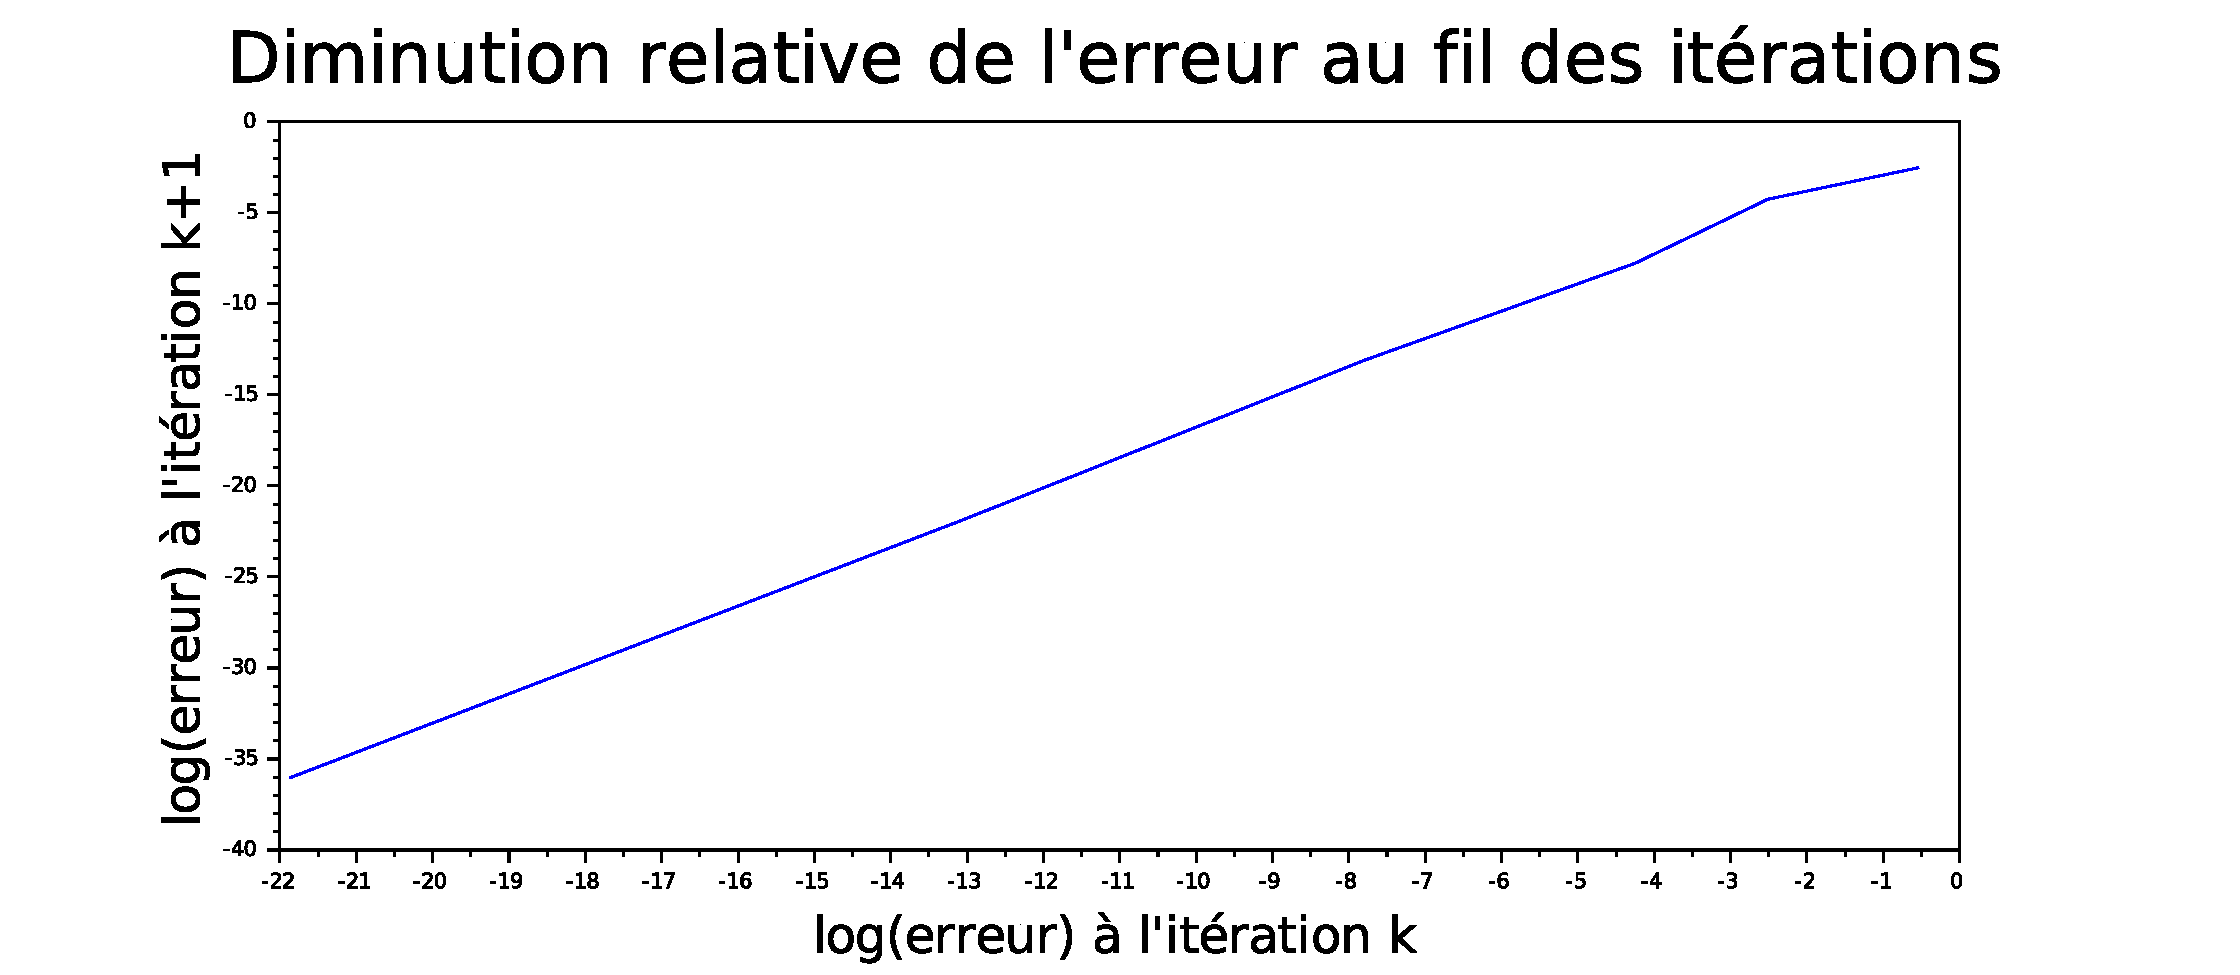
\includegraphics[width=\textwidth]{graphsecante_reg.pdf}
\label{erreur_secante}
\end{figure}
\end{center}

La solution est donc approchée en 7 itérations. Si on linéarise cette courbe (figure \ref{erreur_secante}) grâce à \textit{Scilab}, on obtient un coefficient d'environ 1,6004, il s'agit effectivement d'une convergence d'ordre $\frac{1+\sqrt{5}}{2}$ (le nombre d'or).

\newpage
\section{Pour $n>1$ : La méthode de Newton}
Il existe bien d'autres méthodes afin d'approcher numériquement la solution d'une équations à plusieurs inconnues sous la forme de $f(x) = \left( \begin{array}{c} f_{1}(x) \\ \colon \\ f_{n}(x) \end{array} \right)=0$ avec $f : \mathbb{R} \longrightarrow \mathbb{R}$. La seule méthode dont nous étudierons la partie théorique est la méthode de Newton, appliquée donc dans un cas multidimensionnel.

\subsection{Théorie}
Pour comprendre cette méthode, il apparaît judicieux de revenir sur la notion de différentiabilité. \\
Soit $f : \mathbb{R}^n \longrightarrow \mathbb{R}^n$ avec $f(x) = \left( \begin{array}{c} f_{1}(x) \\ \colon \\ f_{n}(x) \end{array} \right)$ et $x_0\in\mathbb{R}$.\\
On dit que $f$ est différentiable en $x_0$ s'il existe une matrice $A \in \mathcal{M}_{n,n}$ telle que \\
$\forall h\in \mathbb{R}^n$, $f(x_0+h)=f(x_0)+Ah+||h||\varepsilon(h)$ \\ où $\lim\limits_{h \rightarrow \overrightarrow{0}} \varepsilon(h) = \overrightarrow{0}$ et $||h|| \overset{def}{=} \left( \sum \limits_{i=1}^n h_i^2 \right)^\frac{1}{2}$.\\
Les coefficients de $A$ seront alors $a_{i\j}=\frac{\partial f_i}{\partial x_j}(x_0)$.\\
On note $A \overset{def}{=} J_f(x_0)$, $A$ est la matrice Jacobienne de $f$ en $x_0$.\\
\indent De manière analogue au développement de la partie unidimensionnelle, pour $x_0$ donné et $x\in \mathbb{R}$, on a :\\
$f(x)=f(x_0)+J_F(X_0)(x-x_0) + ||x-x_0||\varepsilon(x-x_0)$\\
On effectue l'approximation affine de $f(x)$ : $T_{x_0}(x)=f(x_0)+J_F(x_0)(x-x_0)$\\
On définit $x_1$ par $T_{x_0}(x_1) = \overrightarrow{0}$ (il s'agit d'un système linéaire de n équations à n inconnues)\\
$\Leftrightarrow f(x_0) + J_f(x_0)(x_1-x_0)=\overrightarrow{0} \Leftrightarrow J_f(x_0)(x_1-x_0)=-f(x_0)$\\
d'où $x_1=x_0-\left( J_f(x_0) \right)^{-1}f(x_0)$\\ \\
\indent L'idée de la méthode de Newton est alors la suivante (notons que dans la pratique, on n'inverse pas la matrice, on résout le système d'équation linéaire), pour $x_0$ donné,

\begin{algorithm}
\begin{algorithmic}
\WHILE{$||f(x_n)||>\varepsilon$ \AND $J_{f}(x_{n}) \ est \ inversible$}
\STATE $r\acute{e}soudre \ J_{f}(x_{n})h_{n}=-f(x_{n})$
\STATE $x_{n+1} =  x_{n}+h_{n}$
\ENDWHILE
\end{algorithmic}
\end{algorithm}

\subsection{Fonction \textit{fsolve}}
Avant de commencer l'application de la méthode de Newton, il apparaît judicieux de présenter la macro \textit{fsolve} de \textit{Scilab}. En effet, \textit{Scilab} possède déjà une méthode de résolution des problèmes non linéaires inspirée de la méthode de Newton. \textit{fsolve} a différents prototypes, les arguments qui nous intéressent ici sont :
\begin{itemize}
\item le $x_0$ donné
\item la fonction $f$
\item (facultativement) sa dérivée (\textit{resp.} sa Jacobienne) $df$
\end{itemize}
Si le dernier paramètre, nécessaire à l'application de la méthode de Newton, n'est pas renseigné, \textit{Scilab} ne pouvant la calculer directement, il va l'approcher grâce au développement de Taylor Lagrange.\\
\indent Ainsi, la résolution d'un problème non linéaires avec \textit{Scilab} peut se ramener à la mise en forme du problème sous sa forme standard, $f : \mathbb{R}^n \longrightarrow \mathbb{R}^n$, $f(x)=\overrightarrow{0}$ puis à l'utilisation de la macro \textit{fsolve}.

\subsection{Application 1 : le GPS}

\subsubsection{Énonce et passage en forme standard}
Le sujet de ce problème est le suivant :\\
\indent "Le GPS est un système de positionnement basé sur la connaissance de la distance du récepteur R à trois satellites (situés à des orbites de l’ordre de 	28000km). On suppose que les trois satellites au moment du calcul de distance ont les positions suivantes dans un repère cartésien d’origine le centre de la terre:\\
$S_1 = (-11716.227778, -10118.754628, 21741.083973)$ (unité=km)\\
$S_2 = (-12082.643974, -20428.242179, 11741.374154)$\\
$S_3 = (14373.286650, -10448.439349, 19596.404858)$\\
Sachant que les trois distances respectives au récepteur ont été calculées et valent : $(d_1, d_2, d_3) = (22163.847742, 21492.777482, 21492.469326)$,\\
Déterminer avec \textit{fsolve} la position du récepteur (et vérifier que celui-ci se trouve bien à la surface de la terre...)."\\
\\
\indent Notons $X$ la position du récepteur avec $X= \left( \begin{array}{c} x \\ y \\ z \end{array} \right)$.\\
Le problème nous donne donc le système suivant :
$
\left\lbrace
\begin{array}{l}
||S_1-X||=d_1\\
||S_2-X||=d_2\\
||S_3-X||=d_3\\
\end{array}\right.
$\\
Avec $||X||=\sqrt{x^2+y^2+z^2}$ (il s'agit de la norme euclidienne). La racine carrée pose problème, car la fonction $f : \mathbb{R} \longrightarrow \mathbb{R}$, $f(x)=\sqrt{x}$ n'est pas dérivable sur $\mathbb{R}$. On élève donc chacune des équations du système au carré.
La fonction que l'on cherche donc à annuler dans notre étude est :\\
$f: \mathbb{R}^3 \longrightarrow \mathbb{R}^3$, $f(X)=\left( \begin{array}{c} ||S_1-X||^2-d_1^2 \\ ||S_2-X||^2-d_2^2 \\ ||S_3-X||^2-d_3^2 \end{array} \right)$.\\ \\
\indent Avec \textit{Scilab} comme outils, plusieurs solutions s'offrent donc à nous pour résoudre le problème :
\begin{itemize}
\item utiliser la fonction \textit{fsolve} sans renseigner la Jacobienne
\item calculer la Jacobienne et utiliser la fonction \textit{fsolve} en la renseignant
\item calculer la Jacobienne et appliquer la méthode de Newton (sans utiliser \textit{fsolve})
\end{itemize}
Il peut être intéressant de comparer ces différentes méthodes.

\subsubsection{Méthode 1}
Pour la première méthode, il suffit de renseigner la fonction et de faire appel à \textit{fsolve}. On implémente donc dans \textit{Scilab} le code \ref{GPS1}.

\begin{table}[H]
\caption{GPS (Méthode 1)}
\begin{tabular}{l}
\lstinputlisting[language=scilab]{GPS_1.sce}\\
\end{tabular}
\label{GPS1}
\end{table}

On obtient l'affichage suivant : \begin{verbatim}
-->exec('/home/marlow/latex/GPS_1.sce', -1)
    595.02505  
  - 4856.0251  
    4078.33
\end{verbatim}

\subsubsection{Méthode 2}
Cette méthode ne se différencie pas beaucoup dans la première, la seule différence est que l'on renseigne la Jacobienne en argument de \textit{fsolve}.\\
Calcul de la Jacobienne :\\
Pour simplifier le calcul, on s'intéresse à la première composante de $f(X)$ (à la constante près):\\ $f_1(X) : \mathbb{R}^3 \longrightarrow \mathbb{R}$ avec $f_1(X)=||X-S_1||^2$
\begin{align*}
   f_1(X+h) & = ||(X+h)-S_1||^2 \\
   & = ((X-S_1)+h)^T((X-S_1)+h) \\
   & = (X-S_1)^T(X-S_1) + h^T(X-S_1) + (X-S_1)^Th +h^Th \\
   & = ||X-S_1||^2 + 2(X-S_1)^Th +||h||^2 \\
   & = f_1(X) + J_{f_1}(X) + ||h||\varepsilon(h)
\end{align*}
On peut raisonner de la même façon pour les autres composantes de $f(X)$, on obtient donc :\\
$J_f(X) = \left[ \begin{array}{c} (X-S_1)^T \\ (X-S_2)^T \\ (X-S_3)^T \end{array} \right]$\\
Ainsi, on peut implémenter la Jacobienne dans notre précédent programme \textit{Scilab} et la renseigner dans les arguments de \textit{fsolve}, on obtient le code \ref{GPS2}.

\begin{table}[H]
\caption{GPS (Méthode 2)}
\begin{tabular}{l}
\lstinputlisting[language=scilab]{GPS_2.sce}\\
\end{tabular}
\label{GPS2}
\end{table}

On obtient l'affichage suivant :
\begin{verbatim}
-->exec('/home/marlow/latex/GPS_2.sce', -1)
    595.02505  
  - 4856.0251  
    4078.33   
\end{verbatim}

\subsubsection{Méthode 3}
Enfin, pour tirer parti au maximum de cet exemple, nous allons résoudre le problème sans faire appel à la macro \textit{fsolve} (car \textit{A vaincre sans péril, on triomphe sans gloire}).\\
La Jacobienne a été calculée pour appliquer la deuxième méthode, on a donc : $f(X)=\left( \begin{array}{c} ||S_1-X||^2-d_1^2 \\ ||S_2-X||^2-d_2^2 \\ ||S_3-X||^2-d_3^2 \end{array} \right)$ et
$J_f(X) = \left[ \begin{array}{c} (X-S_1)^T \\ (X-S_2)^T \\ (X-S_3)^T \end{array} \right]$\\
On implémente donc la méthode de Newton dans \textit{Scilab} le code \ref{GPS3}, suivant l'algorithme que nous en avions donné dans la partie théorique.

\begin{table}[H]
\caption{GPS (Méthode 3)}
\begin{tabular}{l}
\lstinputlisting[language=scilab]{GPS_3.sce}\\
\end{tabular}
\label{GPS3}
\end{table}

On obtient l'affichage suivant : \begin{verbatim}
-->exec('/home/marlow/latex/GPS_3.sce', -1)
    595.02505  
  - 4856.0251  
    4078.33    
\end{verbatim}
Cette méthode nous permet de connaître précisément le nombre d'itérations nécessaire pour approcher la solution : $k=10$ après exécution du programme.

\newpage
\subsubsection{Bilan}
Les trois méthodes nous offrent exactement la même solution suivant l'affichage standard de Scilab. On pourrait chercher des différences à quelques décimales prés entre les différentes méthodes, comme on pourrait chercher à connaître le nombre d'itérations (ou d'appels aux fonctions) nécessaires à chaque algorithme avant d'approcher la solution. Toutefois, ce n'est pas vraiment l'objectif qui était fixé, nous nous en tiendrons donc là pour le GPS.\\
Petite remarque : vérifions tout de même que la position que nous avons correspond à une position qui a du sens. En effet, le sujet nous invitait à vérifier que le recepteur se trouve bien à la surface de la Terre : on calcule donc la norme euclidienne de X (notre solution) :
\begin{verbatim}
-->norm(X)
 ans  =
    6369.2864  
\end{verbatim}
Si on suppose un rayon de la Terre égal à 6 371 km (réponse de \textit{Google}), on obtient bien un récepteur GPS à la surface de la Terre.
\\ \\ \\

\subsection{Application 2 : la cinématique inversée}

\subsubsection{Énonce et passage en forme standard}
Le sujet de ce problème est le suivant :\\
\indent "On considère un bras robot articulé dans le plan $(x_1,x_2)$, d’origine $O$, avec un premier segment de longueur $l_1$ et faisant un angle $\theta_1$ avec $(0,x_1)$ et un deuxième segment de longueur $l_2$ faisant un angle $\theta_2$ avec le premier segment. L’extrémité du bras a pour coordonnées :\\
$M(\theta) = (l_1 cos \theta_1 + l_2 cos(\theta_1 + \theta_2 ), l_1 sin \theta_1 + l_2 sin(\theta_1 + \theta_2 ))$.\\
1. Écrire une macro \textit{Scilab} déterminant $\theta$ tel que $M(\theta) = A$ où $A=(x_A,y_A)$ est un point du plan.
2. On prend $l_1 = l_2 = 1$. Écrire un programme \textit{Scilab} utilisant \textit{fsolve} et représentant les positions successives du bras lorsque le point $A(t)$ est défini par une courbe paramétrique, par exemple :\\
$A(t) = \left\lbrace \begin{array}{c} x_1(t)=1+\frac{1}{2}cos(t) \\ x_2(t)=1+\frac{1}{2}sin(t) \end{array} \right.$"\\
\\
\indent Le problème nous donne donc le système suivant :\\
$M(\theta)=A \Leftrightarrow
\left\lbrace
\begin{array}{l}
l_1 cos \theta_1 + l_2 cos(\theta_1 + \theta_2 ) = x_A \\
l_1 sin \theta_1 + l_2 sin(\theta_1 + \theta_2 ) = y_A
\end{array}\right.
$\\
La fonction que l'on cherche donc à annuler dans notre étude est :\\
$f: \mathbb{R}^2 \longrightarrow \mathbb{R}^2$, $f(\theta)=\left( \begin{array}{c} l_1 cos \theta_1 + l_2 cos(\theta_1 + \theta_2 ) - x_A \\ l_1 sin \theta_1 + l_2 sin(\theta_1 + \theta_2 ) - y_A  \end{array} \right)$.\\
\\
Tout comme avec l'application du GPS, plusieurs solutions s'offrent à nous pour résoudre le problème. Toutefois, se contenter d'utiliser la macro \textit{fsolve} ne permet pas d'apprécier l'exécution de la méthode de Newton, itération après itération.

\subsubsection{Calcul de la Jacobienne}
Pour calculer la Jacobienne de la fonction, nous allons utiliser sa définition précédemment énoncée, c'est à dire :\\
$Jf(\theta)=A$ avec $A$ une matrice dont les coefficients sont $a_{i\j}=\frac{\partial f_i}{\partial \theta_j}(\theta)$\\
Par simple calcul de dérivées partielles, on obtient donc :\\
$f(\theta)=\left( \begin{array}{ll}
-l_1 sin \theta_1 - l_2 sin(\theta_1 + \theta_2 ) & -l_2sin(\theta_1+\theta_2) \\
l_1 cos \theta_1 + l_2 cos(\theta_1 + \theta_2 ) & l_2cos(\theta_1+\theta_2)
 \end{array} \right)$

\newpage
\subsubsection{Résolution}
On retranscrit donc à nouveau l'algorithme de la méthode de Newton appliquée à notre exemple dans \textit{Scilab}. On obtient donc le code \ref{code_cinematique}.
\begin{table}[H]
\caption{Cinématique inversée (code principal)}
\begin{tabular}{l}
\lstinputlisting[language=scilab]{cinematique_bis.sce}\\
\end{tabular}
\label{code_cinematique}
\end{table}

\subsubsection{Code fourni pour un rendu graphique}
Le code \textit{dessine\_ bras} appelé pour le rendu graphique est le code \ref{rendu_graphique}.
\begin{table}[H]
\caption{Cinématique inversée (code graphique)}
\begin{tabular}{l}
\lstinputlisting[language=scilab]{dessine_bras.sce}\\
\end{tabular}
\label{rendu_graphique}
\end{table}

\newpage
\subsubsection{Affichage}
On peut ainsi avoir accès après exécution du programme principal à un affichage dynamique de la position du bras à chaque itération. On peut par ailleurs faire varier le nombre d'itérations pour construire plus de bras (figure \ref{affichage_cinematique} : affichages pour différentes valeurs de $n$).
\begin{figure}[H]
\caption{Différents affichages de la cinématique inversée en fonction de $n$}
   \begin{minipage}[c]{.48\linewidth}
   \centering
      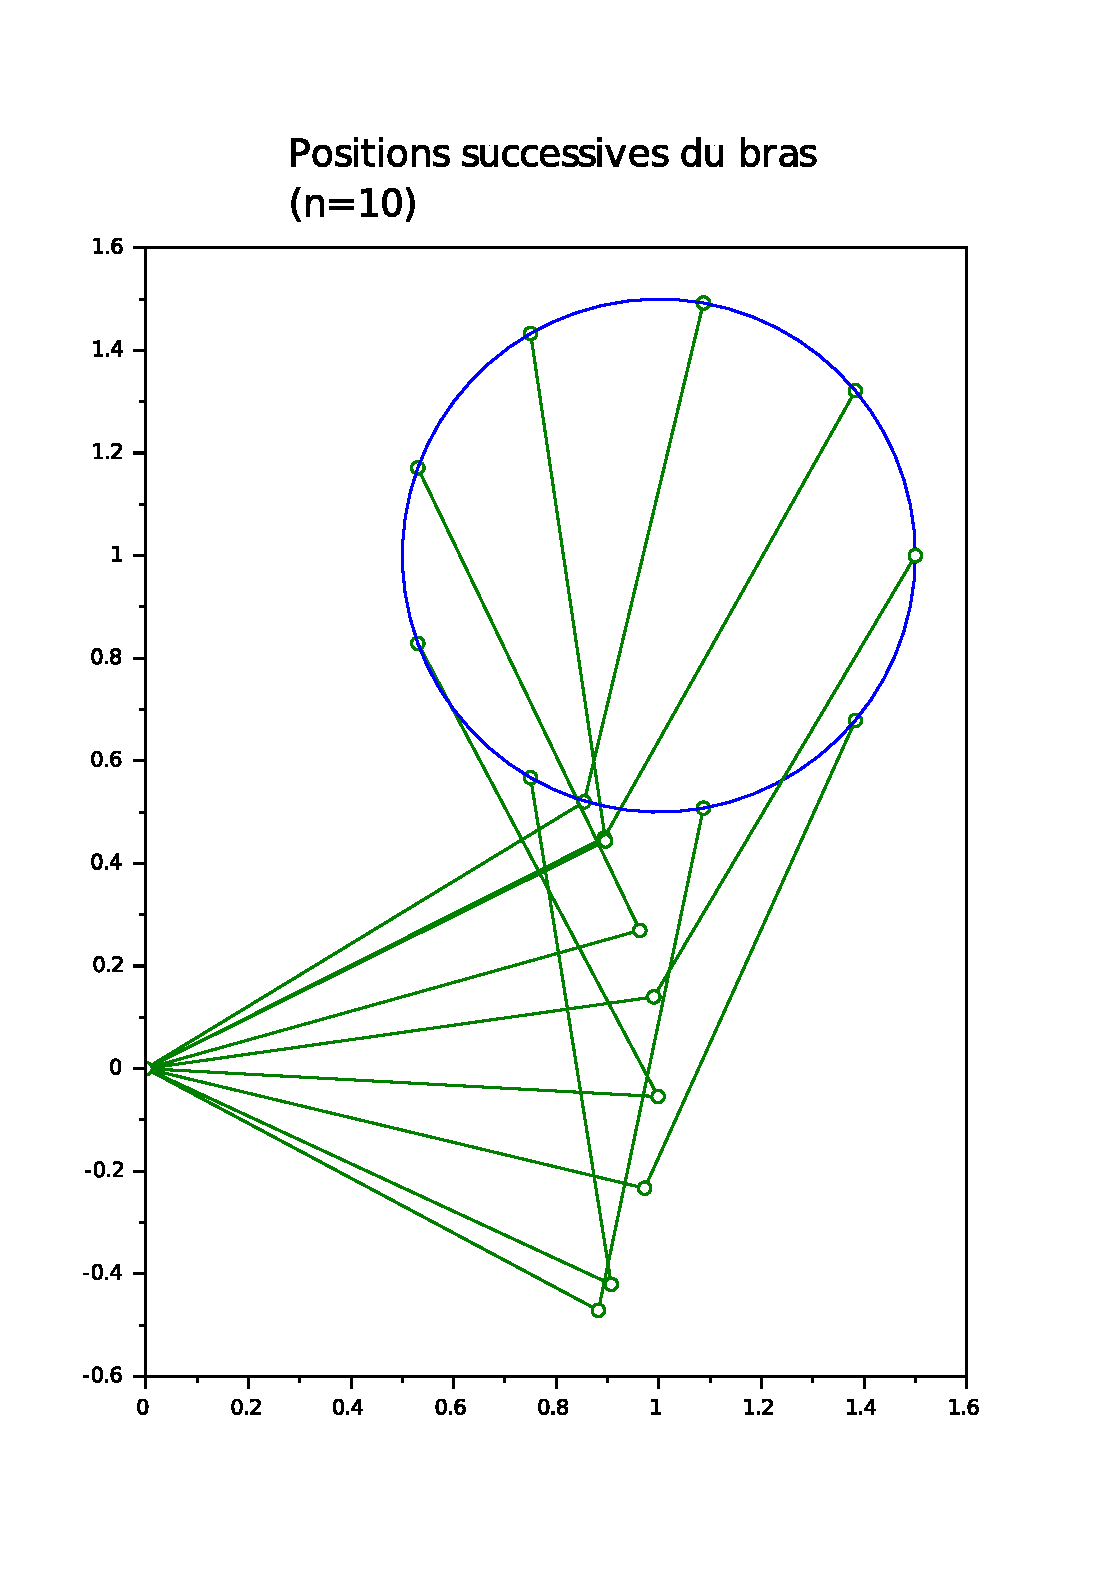
\includegraphics[width=\textwidth]{graphcinematique.pdf}
   \end{minipage} \hfill
   \begin{minipage}[c]{.48\linewidth}
   \centering
      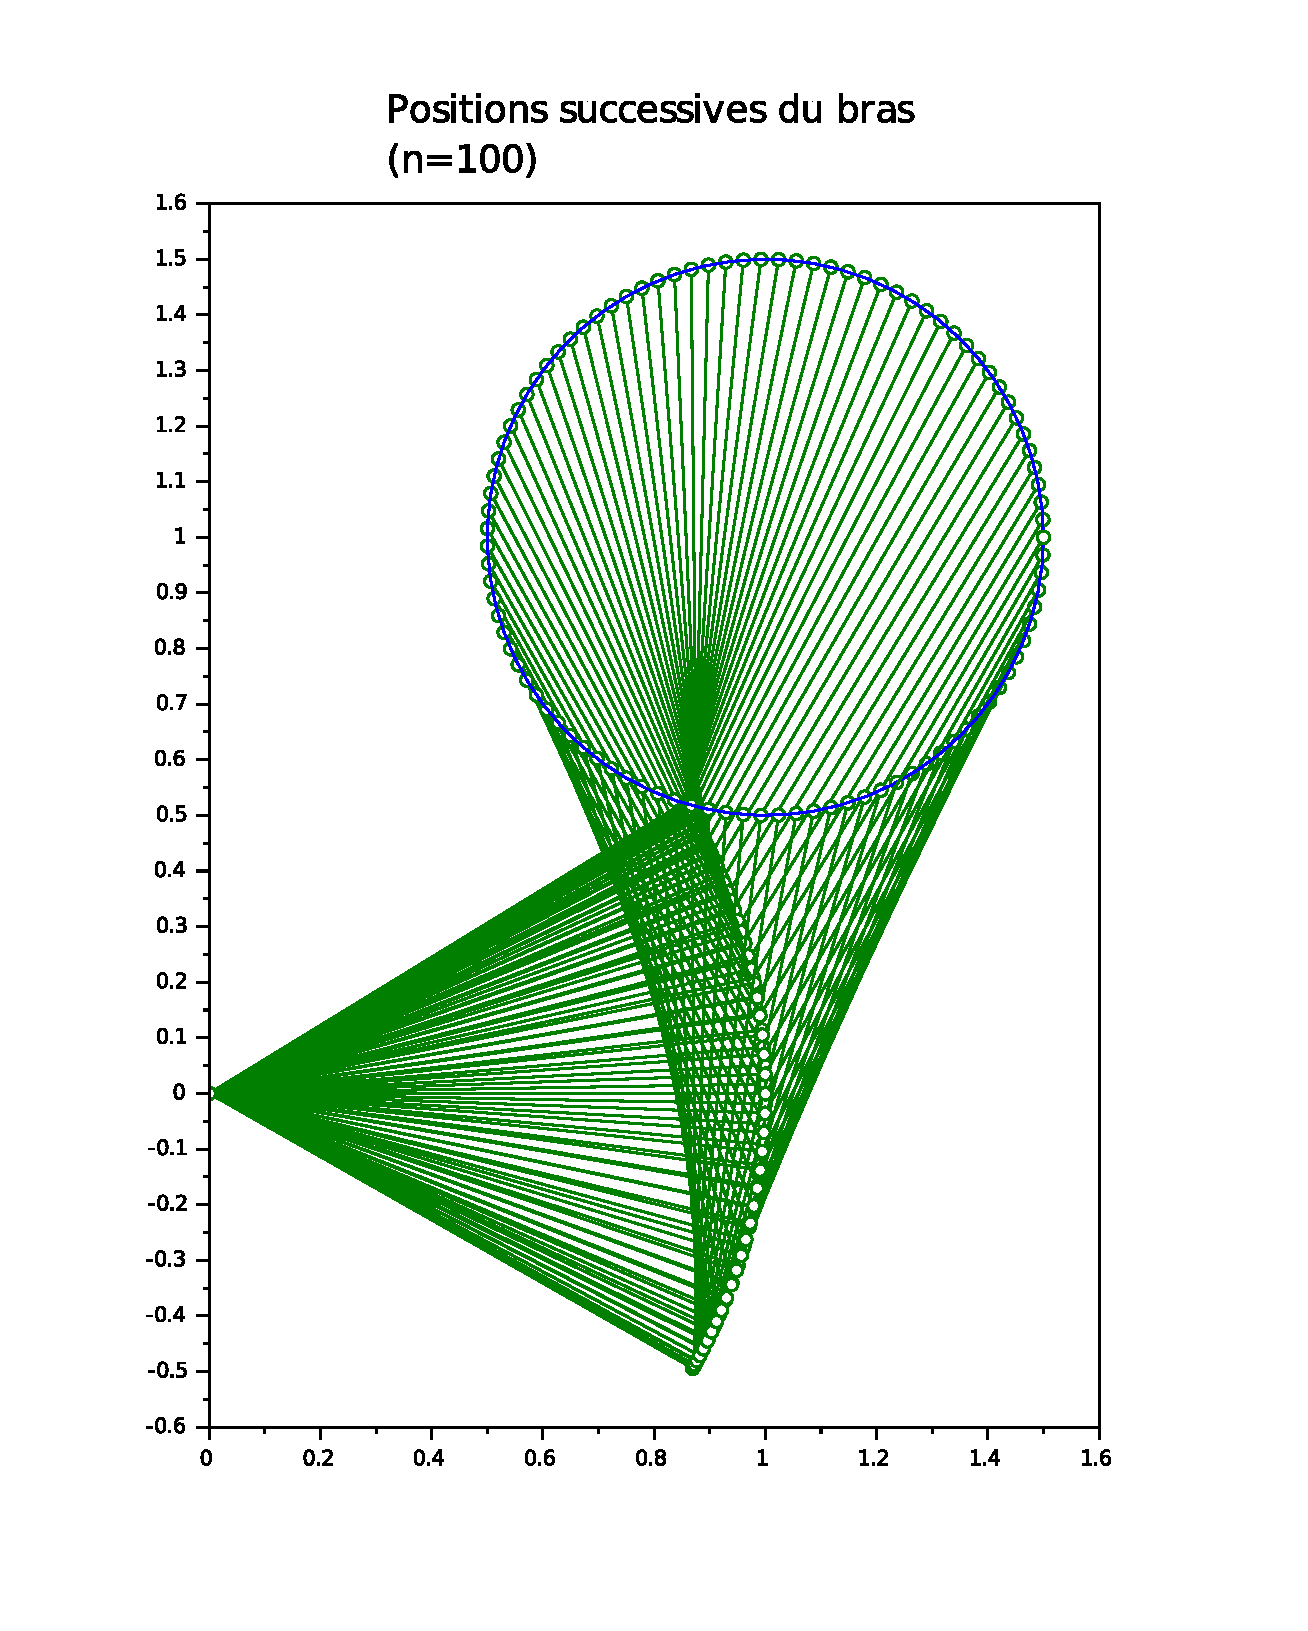
\includegraphics[width=\textwidth]{graphcinematique_2.pdf}
   \end{minipage}
\label{affichage_cinematique}
\end{figure}

\chapter{Fractales}
\section{Introduction}
L'existence des fractales part d'une interrogation assez surprenante : comment construire des figures parfaitement irrégulières, peu importe l'échelle choisie pour les observer (c'est à dire des courbes de fonctions continues mais non dérivables) ? Comment simuler grâce à des outils mathématiques des motifs présent dans la nature comme l'écume des vagues, les nuages,... ? Comment représenter \textit{l'infini} sur une surface finie ? La solution à ces interrogations est d'aller au delà de la géométrie classique, c'est à dire euclidienne.

\begin{center}
\begin{figure}[H]
\caption{Exemple de fractales : fractale de Mandelbrot}
\includegraphics[width=\textwidth]{fractales_intro.jpg}
\end{figure}
\end{center}

\section{Dimension de Hausdorff}
Avant d'étudier des fractales particuliers, il apparaît pertinent de commencer par définir \textit{la dimension de Hausdorff}, c'est à dire la notion de dimension que l'on peut appliquer à un fractal. La dimension de Van Hausdorff d'une fractale $K$ est définie ainsi :\\
\begin{itemize}
\item on note $N(\varepsilon)$ le nombre de carrés de longueur (ou de disques de rayon) $\varepsilon$ recouvrant $K$
\item on a alors $d=\lim\limits_{\varepsilon \rightarrow 0} \frac{ln(N(\varepsilon))}{ln(\frac{1}{\varepsilon})}$, $d \notin \mathbb{N}$
\end{itemize}
Avec cette définition, nous calculerons donc la \textit{dimension de Hausdorff} de chacune des fractales que nous étudierons.

\section{Ensemble de Cantor}
\subsection{Théorie}
\subsubsection{Présentation}
\begin{minipage}[c]{.70\linewidth}
	\indent L'étude de tels objets n'a pas attendu l'apparition du terme "fractale" par Benoît Mandelbrot en 1974. Certains mathématiciens se sont intéressés à 	ces objets avant même de pouvoir les nommer. On considère souvent comme la première figure fractale l'objet construit par le mathématicien allemand Benoît Cantor : \textit{l'ensemble de Cantor}.
	\begin{figure}[H]
	\caption{Ensemble de Cantor}
	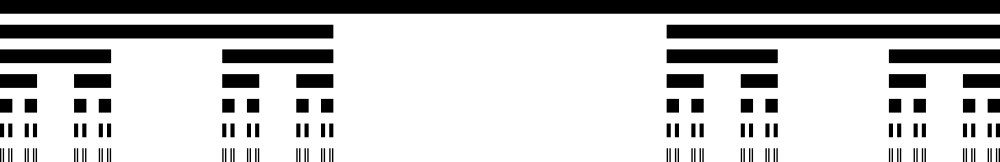
\includegraphics[width=\textwidth]{cantor.png}
	\end{figure}
\end{minipage} \hfill
\begin{minipage}[c]{.05\linewidth}
\end{minipage} \hfill
\begin{minipage}[c]{.21\linewidth}
	\begin{figure}[H]
	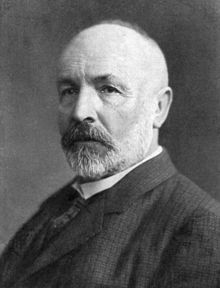
\includegraphics[height=4cm]{mr_cantor.jpg}
	\caption{Cantor 1845-1918}
	\end{figure}
\end{minipage}

\subsubsection{Définition algorithmique}
\begin{algorithm}
\begin{algorithmic}
\REQUIRE{Un segment [0,1]}
\STATE \textbf{Opération de base :} Partager le segment en trois parties égales et ne pas retenir le segment central
\STATE \textbf{Itération :} Itérer l'opération sur chacun des segments retenus
\end{algorithmic}
\end{algorithm}

\subsubsection{Remarques}
On appelle $\mathsf{C^{(k)}}$ l'ensemble obtenu à l'étape $k$, on note : $\mathsf{C^{(\infty)}} = \bigcap^{\infty}_{\mathsf{k}=0}\mathsf{C^{(k)}}$\\
On a par ailleurs les propriétés suivantes :
\begin{align*}
   i) \ & |\mathsf{C^{(\infty)}}|=0 \\
   ii) \ & \mathsf{C^{(\infty)}}\ est\ d\acute{e}nombrable
\end{align*}
On peut démontrer ces propriétés :\\
\textbf{démo \textit{i)}}\\
$|\mathsf{C^{(0)}}|=1$, $|\mathsf{C^{(1)}}|=\frac{2}{3}$, $|\mathsf{C^{(2)}}|=\frac{4}{9}=\left( \frac{2}{3} \right)^2$\\
par récurrence, on obtient $|\mathsf{C^{(k)}}|=\left( \frac{2}{3} \right)^k \Rightarrow \lim\limits_{k \rightarrow \infty} |\mathsf{C^{(k)}}|= 0 \Rightarrow |\mathsf{C^{(\infty)}}|=0$\\

\newpage
\noindent \textbf{démo \textit{ii)}}\\
$\mathsf{C^{(\infty)}}\ est\ en\ bijection\ avec\ [0,1] \Rightarrow \mathsf{C^{(\infty)}}\ est\ d\acute{e}nombrable $\\
Or on a le \textbf{théorème} :\\
$\forall x\in \mathsf{C^{(\infty)}}, x=(0,x_1x_2\cdots x_k\cdots)_3 $ avec $(x)_3$ désigne la base 3 de $x$ et $x_i = 0\ ou\ 2$\\
exemple :
\begin{align*}
   \frac{1}{3} & =(0,1)_3 \ = (0,0222\cdots 2\cdots)_3 = \frac{0}{3} + \frac{2}{3^2} + \frac{2}{3^3} + \cdots + \frac{2}{3^k} + \cdots\\
               & = \frac{2}{3^2} \left( 1 + \frac{1}{3} + \cdots + \frac{1}{3^k} + \cdots \right) = \frac{2}{9} \times \frac{1}{1-\frac{1}{3}} = \frac{2}{9}\times\frac{3}{2}=\frac{1}{3}
\end{align*}
Soit donc la \textbf{bijection} $x \longrightarrow \frac{x}{2}=0,\frac{x_1}{2}\frac{x_2}{2}\cdots\frac{x_k}{2}\cdots$\\
donc $\forall x\in \mathsf{C^{(\infty)}}$ on associe en base 2 le nombre $(0,x_1x_2\cdots x_k\cdots)_2$

\subsubsection{Dimension de l'ensemble de Cantor}
Pour calculer la dimension de l'ensemble de Cantor au sens de la \textit{dimension de Hausdorff}, on compte le nombre de carrés nécessaires à chaque étape pour recouvrir la figure :
\begin{itemize}
\item à l'initialisation, $1$ seul carré de côté $1$
\item à l'itération 1, $2$ carrés de côté $\frac{1}{3}$ sont nécessaires pour recouvrir les segments
\item à l'itération 2, $4=2^2$ carrés de côté $\frac{1}{9} = \frac{1}{3^2}$ sont nécessaires pour recouvrir les segments
\item à l'itération k, $2^k$ carrés de côté $\frac{1}{3^k}$ sont nécessaires pour recouvrir les segments
\end{itemize}
On a donc $d=\lim\limits_{k \rightarrow \infty} \frac{ln(2^k)}{ln(3^k)}=\frac{ln(2)}{ln(3)}$ la dimension de l'ensemble de Cantor.
\\ \\

\subsection{Application dans \textit{Scilab} (méthode récursive)}
La méthode récursive s'inspire directement de l'algorithme de définition de l'ensemble de Cantor. On implémente donc dans \textit{Scilab} le code \ref{code_cantor}.
\begin{table}[H]
\caption{Ensemble de Cantor (méthode récursive)}
\begin{tabular}{l}
\lstinputlisting[language=scilab]{cantor_recursif.sce}\\
\end{tabular}
\label{code_cantor}
\end{table}
L'exécution du code nous donne ainsi la figure \ref{cantor_recursif}.
\begin{center}
\begin{figure}[H]
\centering
\caption{Figure pour n=7}
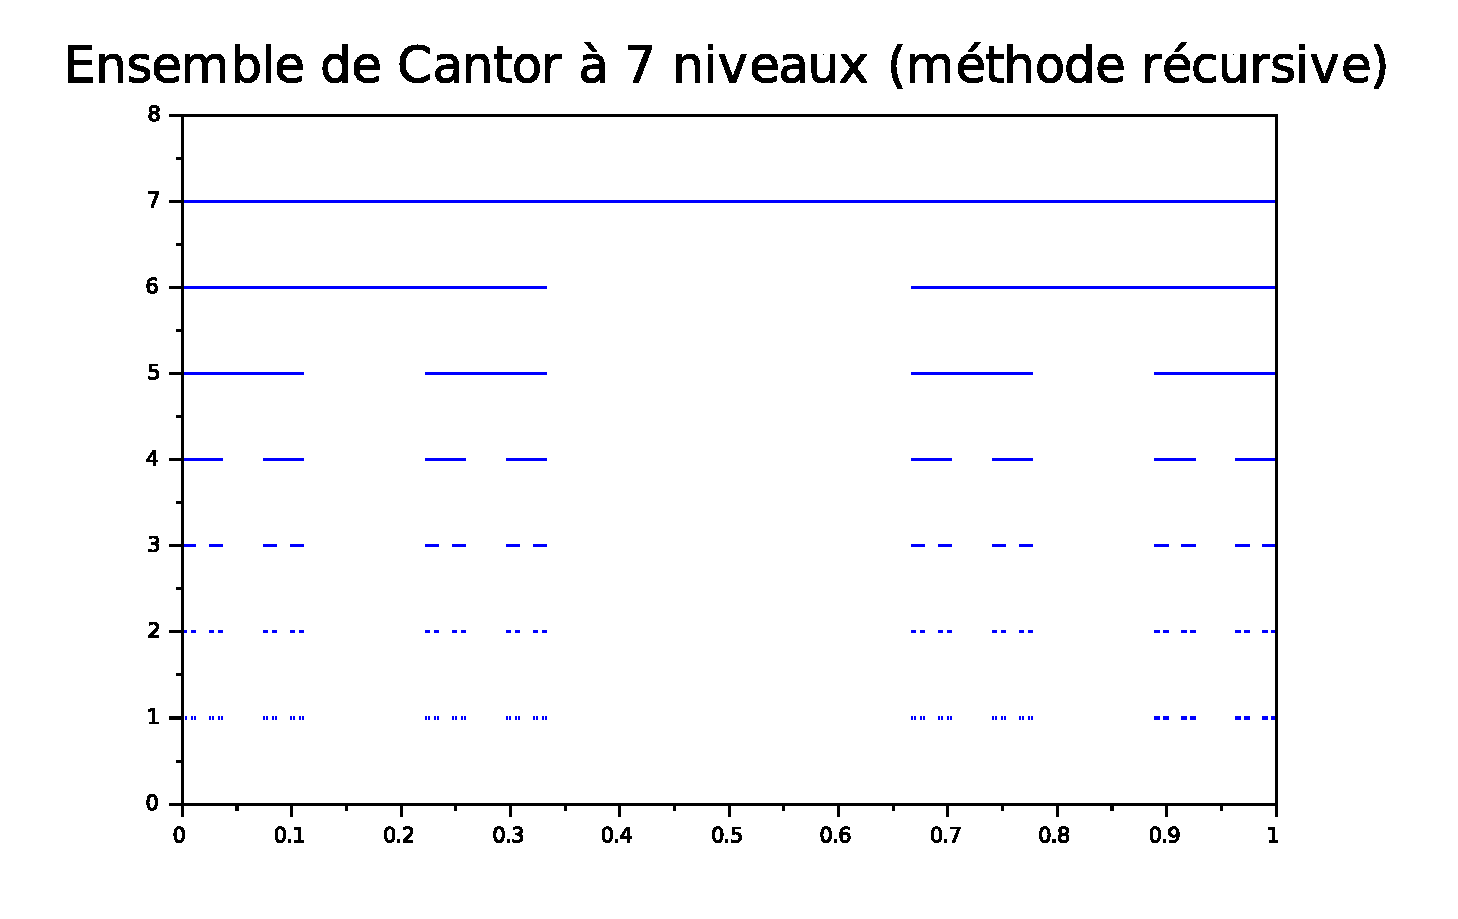
\includegraphics[width=0.8\textwidth]{cantor_recursif.pdf}
\label{cantor_recursif}
\end{figure}
\end{center}

\subsection{Application dans \textit{Scilab} (méthode itérative)}
Même si la méthode récursive appliquée précedemment pour dessiner l'ensemble de Cantor s'est révélée efficace pour $n=7$ niveaux, elle l'est beaucoup moins pour des valeurs de $n$ supérieures. En effet, la complexité de l'algorithme est de l'ordre de $O(2^n)$ (on réalise 2 appels récursifs pour chaque niveau), on dit qu'elle est exponentielle, un tel algorithme est donc de plus en plus \textit{gourmand} en temps et en mémoire à mesure que $n$ augmente. En outre, la complexité des algorithmes récursifs devient rapidement délirante pour tracer des fractales en 2D, encore d'avantage en 3D. C'est pourquoi il est pertinent de s'intéresser dés à présent à d'autres méthodes de dessin des fractales : les méthodes itératives. Nous allons donc étudier l'une d'entre elles : celles des IFS (\textit{Iterated Functions Systems}), en français \textit{les systèmes de fonctions itérées}.\\
\\
\indent La théorie des IFS, basée sur l'invariance par changement d'échelle, permet la représentation fonctionnelle d'un fractale. Cette théorie fait appel à la notion de \textit{fonctions contractantes} sur un espace métrique $M$, (c'est à dire muni d'une notion de distance $d$ entre deux éléments). Graphiquement, une fonction contractante "rapproche les images". Une fonction $f$ est dite \textit{contractante} ou \textit{k-contractante} sur $M(E,d)$ ssi :
\begin{equation}
\exists k, 0\leq k\leq 1, \forall (x,y) \in E^2, d(f(x),f(y))\leq kd(x,y)
\end{equation}
\indent Un IFS est un ensemble de fonctions $f_1,f_2,\cdots f_n$ toutes contractantes sur un ensemble de compacts de $M$ munis de la \textit{distance de Hausdorff}. On définit alors la fonction $f$, avec $A$ un compact, par :
\begin{equation}
f(A)=f_1(A)\cup f_2(A)\cup \cdots \cup f_n(A)
\end{equation}
On peut montrer que $f$ est aussi contractante de rapport de contraction $k=max(k_i)$.

\indent Le \textit{théorème du collage}, démontré par Barnsley en 1985, énonce que tout IFS converge vers un \textit{attracteur} $A$, c'est à dire un ensemble vers lequel le système évolue irrémédiablement, tel que $f(A)=A$ pour tout donnée initiale choisie, $A$ est donc un point fixe de $f$. Autrement dit, un IFS converge vers un compact attracteur $A$ qui se révèle être une fractale.
\\ \\
\indent Pour une fractale particulière, on déduit les fonctions $f_1,f_2,\cdots f_n$ à partir de la définition algorithmique de la fractale. On travaille donc sur un ensemble fini de points, et pour chaque point, on choisit (aléatoirement) d'y appliquer une des fonctions $f_1,f_2,\cdots f_n$. \\

Pour l'ensemble de Cantor, on a :\\
\begin{equation}
\begin{array}{l}
f(C)=f_0(C)\cup f_1(C) \ avec \
\left\lbrace
\begin{array}{l}
f_0,\ f_1 : [0,1] \longrightarrow [0,1] \\
f_0 : x \longrightarrow \frac{x}{3}\\
f_1 : x \longrightarrow \frac{x}{3}+\frac{2}{3}\\
\end{array}\right.
d'o\grave{u} \
\left\lbrace
\begin{array}{l}
C_0 : [0,1]\\
C_{n+1} : f(C_n)\\
\end{array}\right.
\end{array}
\end{equation}
Finalement $C_n$ converge au sens de la distance de Hausdorff vers $C^\infty$, l'ensemble de Cantor. Pour la sélection de la fonction à appliquer à une point particulier, on applique une méthode équiprobable afin d'obtenir un ensemble uniforme.\\ \\
\indent On implémente donc dans \textit{Scilab} le code suivant :
\begin{table}[H]
\caption{Ensemble de Cantor (méthode itérative)}
\begin{tabular}{l}
\lstinputlisting[language=scilab]{cantor_iteratif.sce}\\
\end{tabular}
\end{table}
L'exécution du code nous donne ainsi la figure \ref{cantor_iteratif}.:
\begin{center}
\begin{figure}[H]
\caption{Ensemble de Cantor itératif pour 1000 points}
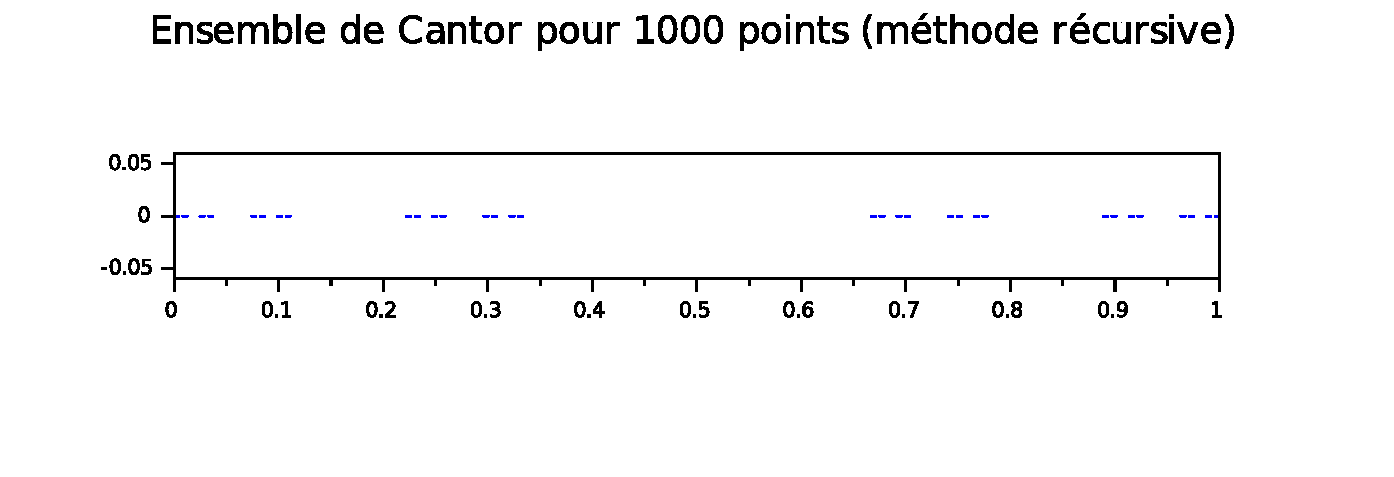
\includegraphics[width=\textwidth]{cantor_iteratif.pdf}
\label{cantor_iteratif}
\end{figure}
\end{center}

\section{Triangle de Sierpinski}
\subsection{Théorie}
\subsubsection{Présentation}
\begin{minipage}[c]{.70\linewidth}
	\indent Notre analyse continue avec l'étude d'une seconde fractale construite par Waclaw Sierpinski, mathématicien polonais, fractale nommée \textit{le triangle de Sierpinski}.
	\begin{figure}[H]
	\centering
	\caption{Triangle de Sierpinski}
	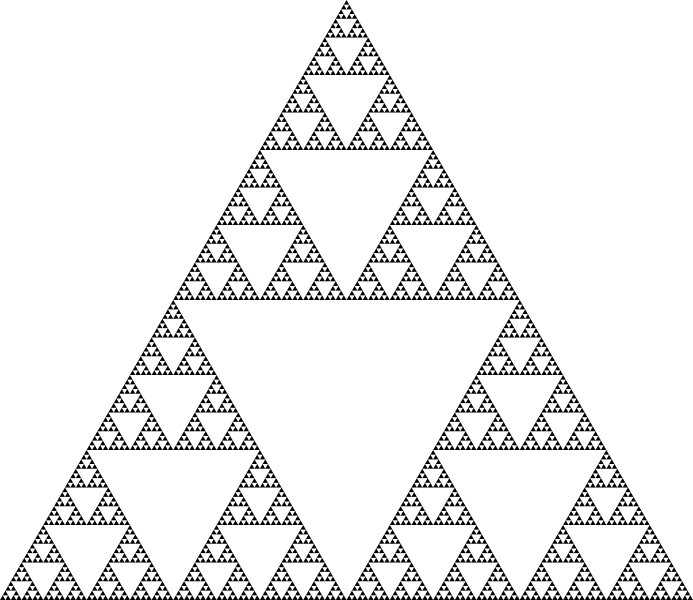
\includegraphics[height=5cm]{sierpinski.png}
	\end{figure}
\end{minipage} \hfill
\begin{minipage}[c]{.05\linewidth}
\end{minipage} \hfill
\begin{minipage}[c]{.21\linewidth}
	\begin{figure}[H]
	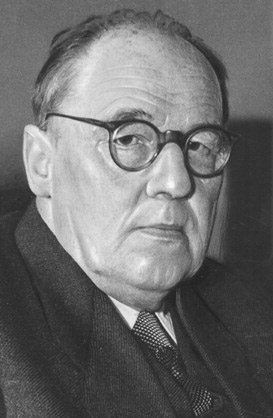
\includegraphics[height=4cm]{mr_sierpinski.jpg}
	\caption{Sierpinski 1882-1924}
	\end{figure}
\end{minipage}

\subsubsection{Définition algorithmique}
\begin{algorithm}
\begin{algorithmic}
\REQUIRE{Un triangle équilatéral de côté 1}
\STATE \textbf{Opération de base :} Partager le triangle en 4 triangles équilatéraux égaux et ne pas retenir le triangle central
\STATE \textbf{Itération :} Itérer l'opération sur chacun des triangles retenus
\end{algorithmic}
\end{algorithm}

\subsubsection{Dimension du Triangle de Sierpinski}
On appelle $T^k$ la figure obtenue à l'itération $k$. On applique donc la définition de la dimension de Hausdorff au triangle de Sierpinski :\\ \\
\begin{tabular}{ccccc}
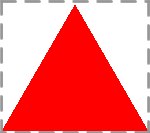
\includegraphics[height=2.4cm]{sierpinski0.png} & $\rightarrow$ & 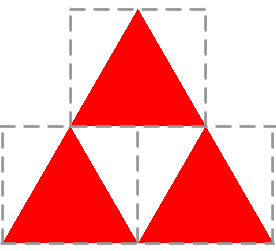
\includegraphics[height=2.5cm]{sierpinski1.png} & $\rightarrow$ & 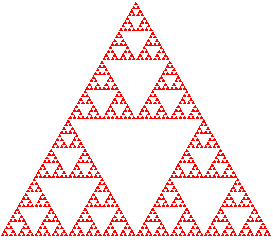
\includegraphics[height=2.5cm]{sierpinskik.png}\\
$T_0$ & & $T_1$ & ... & $T_k$\\
1 seul carré & & 3 carrés & ... & $3^k$ carrés\\
de côté 1 & & de côté $\frac{1}{2}$ & ... & de côté $\varepsilon_k = \frac{1}{2^k}$\\
\end{tabular} \\ \\ \\
Donc $d=\lim\limits_{k \rightarrow \infty} \frac{ln(3^k)}{ln(2^k)}=\frac{ln(3)}{ln(2)}$ est la dimension de Hausdorff du fractal.

\newpage
\subsection{Application dans \textit{Scilab} (méthode récursive)}
Le programme récursif s'inspire tout autant de la définition même de la fractale que celui pour l'ensemble de Cantor. On implémente donc dans \textit{Scilab} le code \ref{code_sierp}.
\begin{table}[H]
\caption{Triangle de Sierpinski (méthode récursive)}
\begin{tabular}{l}
\lstinputlisting[language=scilab]{sierpinski_recursif.sce}\\
\end{tabular}
\label{code_sierp}
\end{table}
L'exécution du code nous donne ainsi la figure \ref{sierpinski_recursif}.
\begin{figure}[H]
\centering
\caption{Triangle de Sierpinski (récursif) pour n=5}
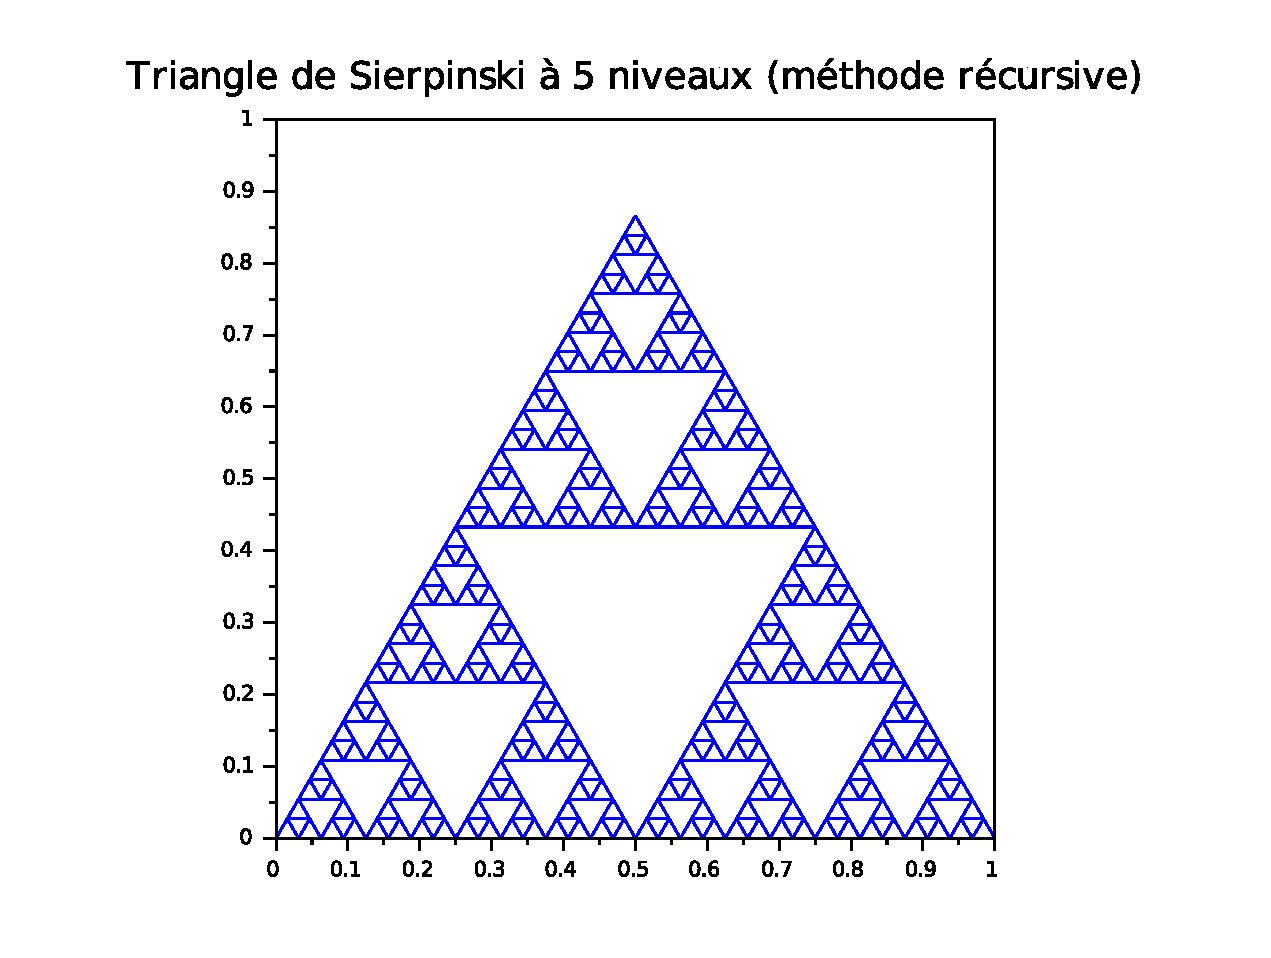
\includegraphics[width=0.75\textwidth]{sierpinski_recursif.pdf}
\label{sierpinski_recursif}
\end{figure}

\newpage
\subsection{Application dans \textit{Scilab} (méthode itérative)}
La complexité de l'algorithme récursif est ici en $O(3^n)$ (on réalise 3 appels récursifs pour chaque niveau). Comme pour l'ensemble de Cantor, cette complexité est surmontable pour des valeurs de niveaux relativement faibles ($n\leq 7$), mais pour des valeurs de $n$ importantes, cette méthode n'est plus applicable. On implémente donc également une méthode itérative à l'aide d'un IFS. On a donc :
\begin{equation}
\left\lbrace
\begin{array}{l}
f_0 \left[ \begin{array}{ll} x \\ y \end{array} \right] =
\left[ \begin{array}{ll} \frac{1}{2} & 0 \\ 0 & \frac{1}{2} \end{array} \right]
\left[ \begin{array}{ll} x \\ y \end{array} \right]\\ \\

f_1 \left[ \begin{array}{ll} x \\ y \end{array} \right] =
\left[ \begin{array}{ll} \frac{1}{2} & 0 \\ 0 & \frac{1}{2} \end{array} \right]
\left[ \begin{array}{ll} x \\ y \end{array} \right]
+ \left[ \begin{array}{ll} \frac{1}{2} \\ 0 \end{array} \right]\\ \\

f_2 \left[ \begin{array}{ll} x \\ y \end{array} \right] =
\left[ \begin{array}{ll} \frac{1}{2} & 0 \\ 0 & \frac{1}{2} \end{array} \right]
\left[ \begin{array}{ll} x \\ y \end{array} \right]
+ \left[ \begin{array}{ll} \frac{1}{4} \\ \frac{\sqrt{3}}{4} \end{array} \right]\\
\end{array}\right.
\end{equation}
$d'o\grave{u} \
\left\lbrace
\begin{array}{l}
T_0 \ donn\acute{e} \\
T_{n+1} : f(T_n) \ avec \ f(T)=f_0(T)\cup f_1(T)\cup f_2(T)\\
\end{array}\right.$\\ \\
Finalement $T_n$ converge au sens de la distance de Hausdorff vers $T^\infty$, le triangle de Sierpinski. A nouveau, la dispersion des points doit être uniforme, on utilise donc des conditions d'équiprobabilité. \\ \\

\indent On implémente donc dans \textit{Scilab} le code \ref{code_sierpinski_it}.
\begin{table}[H]
\caption{Triangle de Sierpinski (méthode itérative)}
\begin{tabular}{l}
\lstinputlisting[language=scilab]{sierpinski_iteratif.sce}\\
\end{tabular}
\label{code_sierpinski_it}
\end{table}
\newpage
L'exécution du code nous donne ainsi la figure \ref{sierpinski_iteratif}.
\begin{figure}[H]
\centering
\caption{Triangle de Sierpinski itératif pour 1000 points}
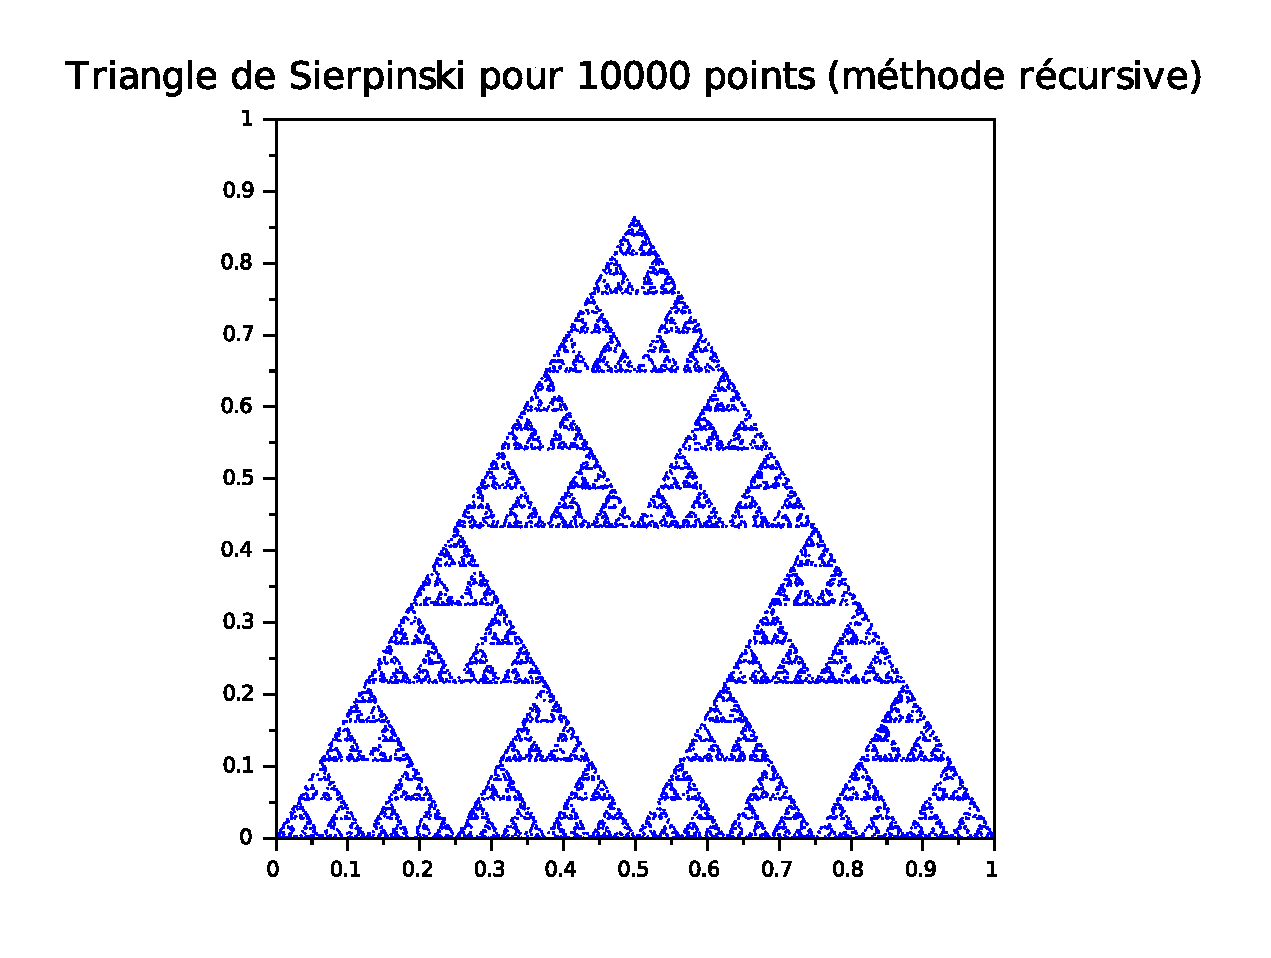
\includegraphics[width=0.75\textwidth]{sierpinski_iteratif.pdf}
\label{sierpinski_iteratif}
\end{figure}

\subsection{Variante : le tapis de Sierpinski}
On a pu travailler sur une variante du triangle de Sierpinski : \textit{Le tapis de Sierpinski}.
\begin{figure}[H]
\centering
\caption{Tapis de Sierpinski}
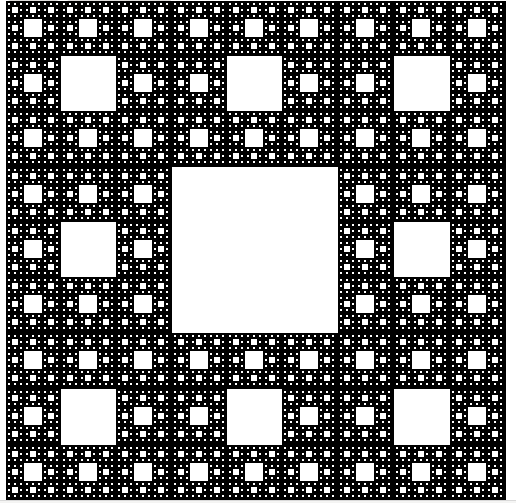
\includegraphics[width=7cm]{tapis.png}
\label{tapis_rec}
\end{figure}

Largement similaire au triangle, on implémente le code \ref{code_tapis_rec} (méthode récursive).

\begin{table}[H]
\caption{Tapis de Sierpinski (méthode récursive)}
\begin{tabular}{l}
\lstinputlisting[language=scilab]{tapis_sierpinski_recursif.sce}\\
\end{tabular}
\label{code_tapis_rec}
\end{table}

L'exécution du code nous donne ainsi la figure \ref{tapis_rec}.
\begin{figure}[H]
\centering
\caption{Tapis de Sierpinski (récursif) pour n=2}
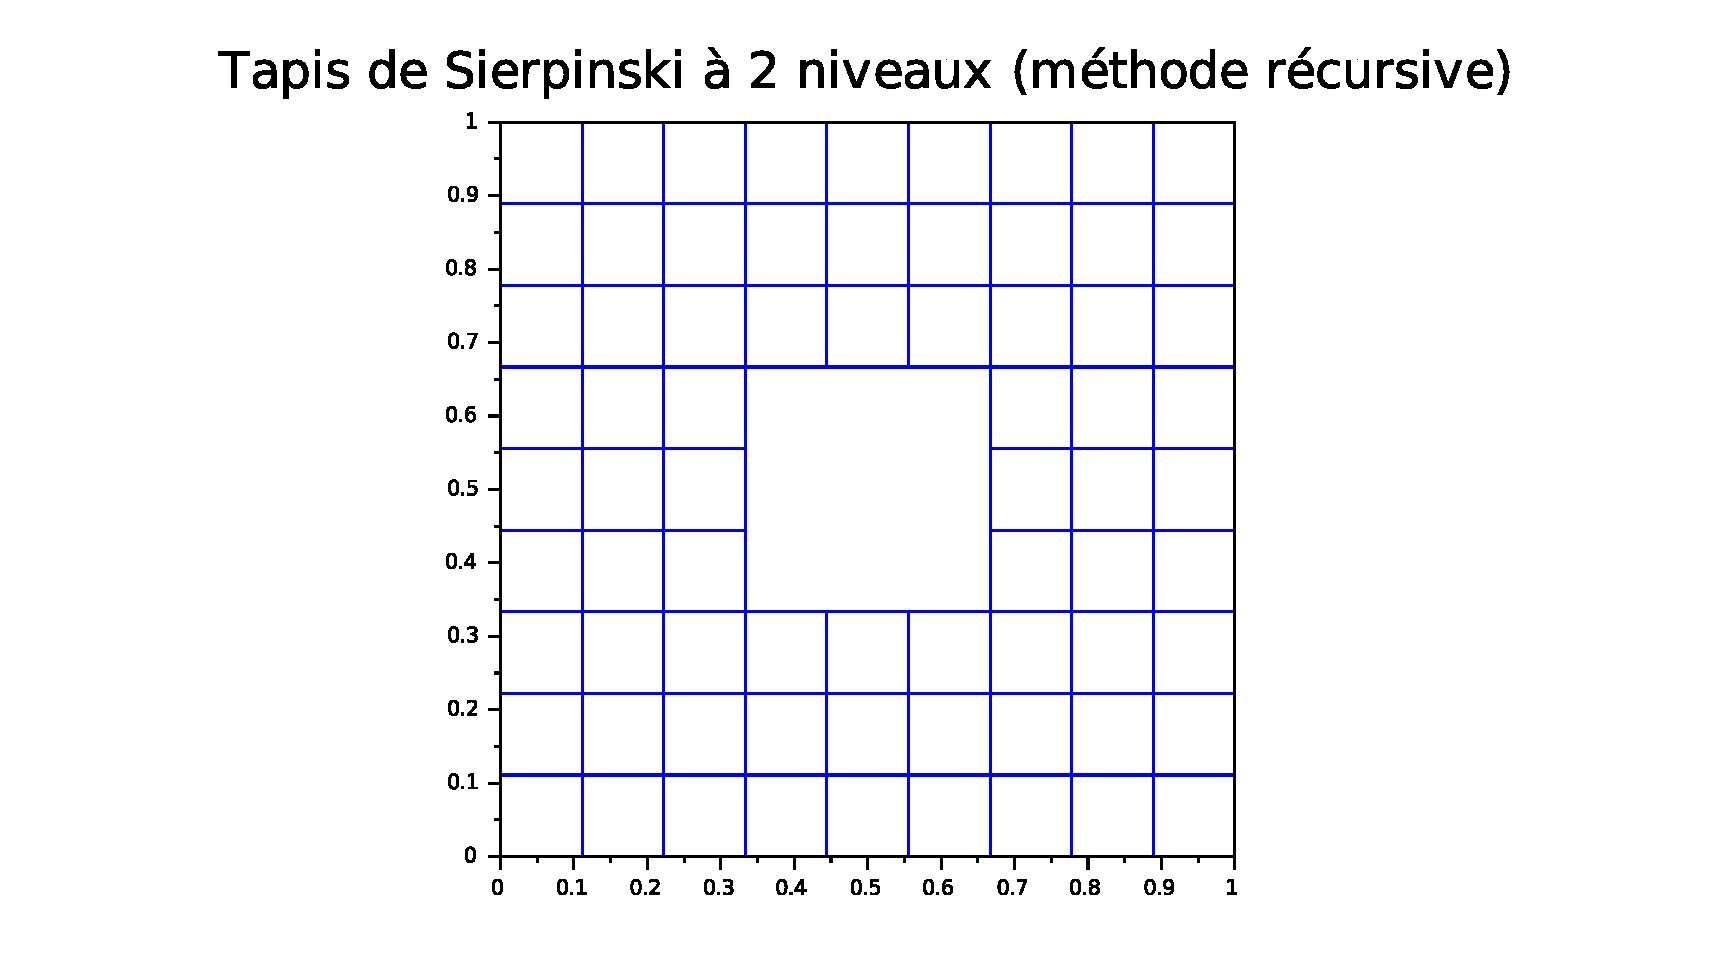
\includegraphics[width=0.75\textwidth]{tapis_recursif.pdf}
\label{tapis_rec}
\end{figure}

\newpage
On obtient donc un algorithme récursif de complexité en $O(8^n)$, complexité difficilement supportable pour la machine (mon ordinateur ne parvient à dessiner dans un temps raisonnable que le niveau $n=2$...). On implémente donc également la méthode itérative avec le code \ref{code_tapis_it} suivant l'IFS :

\begin{equation}
\left\lbrace
\begin{array}{lll}
f_1 \left[ \begin{array}{l} x \\ y \end{array} \right] =
\left[ \begin{array}{ll} \frac{1}{3} & 0 \\ 0 & \frac{1}{3} \end{array} \right]
\left[ \begin{array}{l} x \\ y \end{array} \right]
& &
f_2 \left[ \begin{array}{l} x \\ y \end{array} \right] =
\left[ \begin{array}{ll} \frac{1}{3} & 0 \\ 0 & \frac{1}{3} \end{array} \right]
\left[ \begin{array}{l} x \\ y \end{array} \right]
+ \left[ \begin{array}{l} \frac{1}{3} \\ 0 \end{array} \right]\\ \\

f_3 \left[ \begin{array}{l} x \\ y \end{array} \right] =
\left[ \begin{array}{ll} \frac{1}{3} & 0 \\ 0 & \frac{1}{3} \end{array} \right]
\left[ \begin{array}{l} x \\ y \end{array} \right]
+ 2 \times \left[ \begin{array}{l} \frac{1}{3} \\ 0 \end{array} \right]
& &
f_4 \left[ \begin{array}{l} x \\ y \end{array} \right] =
\left[ \begin{array}{ll} \frac{1}{3} & 0 \\ 0 & \frac{1}{3} \end{array} \right]
\left[ \begin{array}{l} x \\ y \end{array} \right]
+ \left[ \begin{array}{l} 0 \\ \frac{1}{3} \end{array} \right]\\ \\

f_5 \left[ \begin{array}{l} x \\ y \end{array} \right] =
\left[ \begin{array}{ll} \frac{1}{3} & 0 \\ 0 & \frac{1}{3} \end{array} \right]
\left[ \begin{array}{l} x \\ y \end{array} \right]
+ 2 \times \left[ \begin{array}{l} \frac{1}{3} \\ 0 \end{array} \right] + \left[ \begin{array}{l} 0 \\ \frac{1}{3} \end{array} \right]
& &
f_6 \left[ \begin{array}{l} x \\ y \end{array} \right] =
\left[ \begin{array}{ll} \frac{1}{3} & 0 \\ 0 & \frac{1}{3} \end{array} \right]
\left[ \begin{array}{l} x \\ y \end{array} \right]
+ \left[ \begin{array}{l} \frac{1}{3} \\ 0 \end{array} \right]\\ \\

f_7 \left[ \begin{array}{l} x \\ y \end{array} \right] =
\left[ \begin{array}{ll} \frac{1}{3} & 0 \\ 0 & \frac{1}{3} \end{array} \right]
\left[ \begin{array}{l} x \\ y \end{array} \right]
+ \left[ \begin{array}{l} \frac{1}{3} \\ 0 \end{array} \right] + 2 \times \left[ \begin{array}{l} 0 \\ \frac{1}{3} \end{array} \right] & &\\ \\
f_8 \left[ \begin{array}{l} x \\ y \end{array} \right] =
\left[ \begin{array}{ll} \frac{1}{3} & 0 \\ 0 & \frac{1}{3} \end{array} \right]
\left[ \begin{array}{l} x \\ y \end{array} \right]
+ 2 \times \left[ \begin{array}{l} \frac{1}{3} \\ 0 \end{array} \right] + 2 \times \left[ \begin{array}{l} 0 \\ \frac{1}{3} \end{array} \right]
\end{array}\right.
\end{equation}

\begin{table}[H]
\caption{Tapis de Sierpinski (méthode itérative)}
\begin{tabular}{l}
\lstinputlisting[language=scilab]{tapis_sierpinski_recursif.sce}\\
\end{tabular}
\label{code_tapis_it}
\end{table}

L'exécution du code nous donne ainsi la figure \ref{tapis_it}.
\begin{figure}[H]
\centering
\caption{Tapis de Sierpinski (itératif) pour n=100000 points}
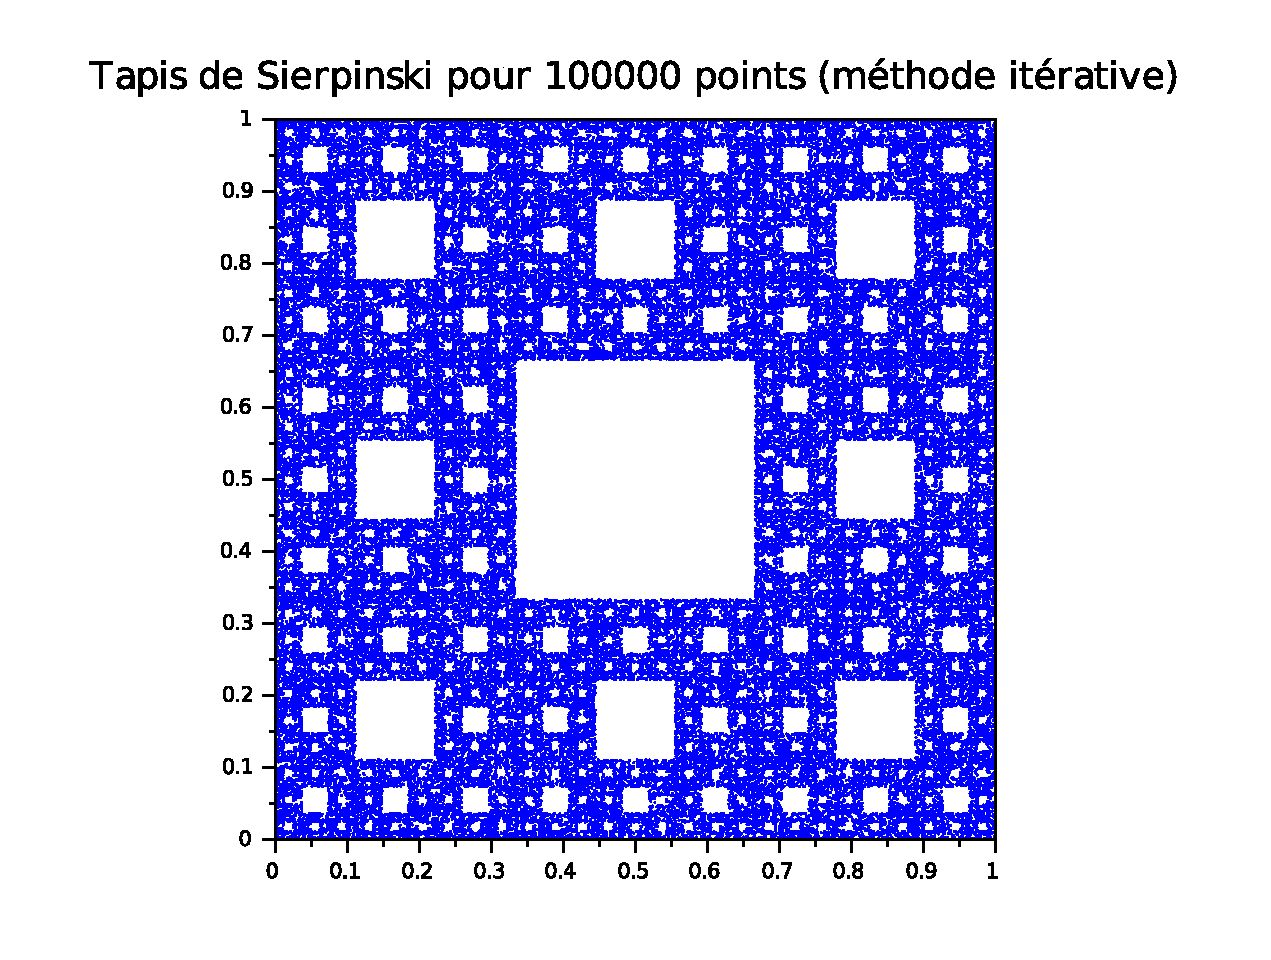
\includegraphics[width=0.75\textwidth]{tapis_iteratif.pdf}
\label{tapis_it}
\end{figure}


\section{Flocon de neige de Von Koch}
\subsection{Théorie}
\subsubsection{Présentation}
\begin{minipage}[c]{.70\linewidth}
	\indent Notre analyse continue avec l'étude d'une troisième fractale construite par Helge Von Koch, mathématicien suédois, fractale nommée le \textit{flocon de Von Koch}.
	\begin{figure}[H]
	\centering
	\caption{Flocon de neige de Von Koch}
	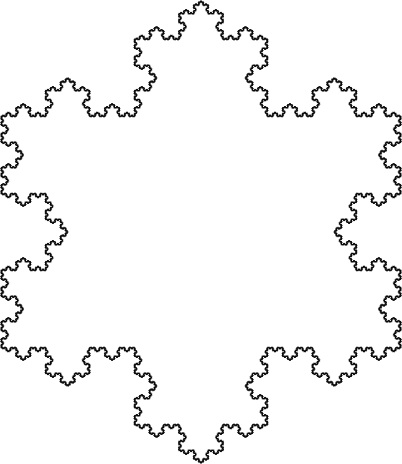
\includegraphics[width=6cm]{koch.jpg}
	\end{figure}
\end{minipage} \hfill
\begin{minipage}[c]{.05\linewidth}
\end{minipage} \hfill
\begin{minipage}[c]{.21\linewidth}
	\begin{figure}[H]
	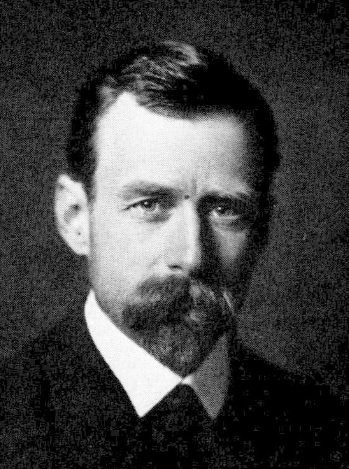
\includegraphics[height=4cm]{mr_koch.png}
	\caption{Von Koch 1870-1924}
	\end{figure}
\end{minipage}

\newpage
\subsubsection{Définition algorithmique}
\begin{algorithm}
\begin{algorithmic}
\REQUIRE{Un triangle équilatéral de côté 1}
\STATE \textbf{Opération de base :} Chaque segment du triangle est partagé en 3 parties égales.\\
Le segment central $S_C$ est remplacé par 2 segments égaux formant un triangle équilatéral ayant pour base $S_C$
\STATE \textbf{Itération :} Itérer l'opération sur chacun des segments obtenus
\end{algorithmic}
\end{algorithm}

\subsubsection{Remarques}
A l'infini, on obtient donc $\mathsf{K^{(\infty)}}$ le flocon de Van Koch. On a en outre les propriétés suivantes :\\
\begin{align*}
   i) \ & l(\mathsf{K^{(\infty)}})=+\infty \\
   ii) \ & \mathit{A}(\mathsf{K^{(\infty)}})<\infty
\end{align*}
En effet :\\
\textbf{longueur :}\\
\begin{tabular}{cccccc}
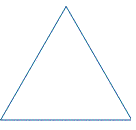
\includegraphics[height=2cm]{koch_l0.png} & $\rightarrow$ & 
\includegraphics[height=2cm]{koch_l1.png} & $\rightarrow$ & 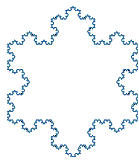
\includegraphics[height=2cm]{koch_k.png} &\\
$l_0=3$ & & $l_1=12\times \frac{1}{3}=4$ & ... & $l_k=4^k$ & $\overset{k \rightarrow +\infty}{\longrightarrow} +\infty $\\
\end{tabular} \\ \\ \\
\textbf{aire :}\\
\begin{tabular}{ccccc}
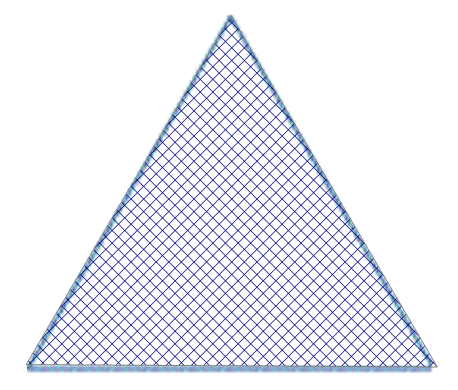
\includegraphics[height=2cm]{koch_a0.png} & $\rightarrow$ & 
\includegraphics[height=2cm]{koch_a1.png} & $\rightarrow$ & 
$
\left\lbrace
\begin{array}{l}
A_2 = A_1 + \frac{12A_0}{3^4}=A_1+\frac{2^2}{3^3}A_0 \\
\\
A_3 = A_2 + \frac{48A_0}{3^6}=A_1+\frac{2^4}{3^5}A_0
\end{array}\right.
 $\\
$A_0$ & & $A_1=A_0 + \frac{3A_0}{9}$ & & \\
&&$=A_0 + \frac{A_0}{3}$&&\\
\end{tabular} \\ \\ \\
donc $A_k=A_0+A_0\frac{1}{3}+A_0\frac{2^2}{3^3}+A_0\frac{2^4}{3^5}+\cdots + A_0\frac{2^{2k}}{3^{2k+1}}$\\
à l'infini, on a donc : $A_{\infty}=A_0+ \sum \limits_{k=0}^\infty \frac{2^{2k}}{3^{2k+1}} = A_0 + \frac{A_0}{3}\sum \limits_{k=0}^\infty \left( \frac{2}{3} \right)^{2k}$ = ?

\subsubsection{Dimension du Flocon de Von Koch}
On applique donc la définition de la dimension de Hausdorff au flocon de Von Koch :\\ \\
\begin{tabular}{ccccc}
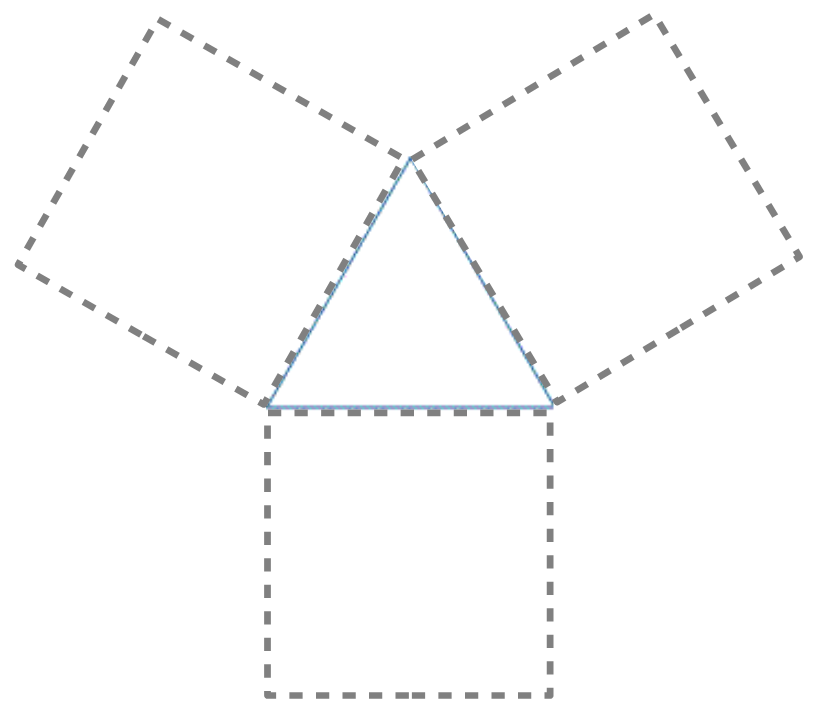
\includegraphics[height=2.4cm]{koch_0.png} & $\rightarrow$ & 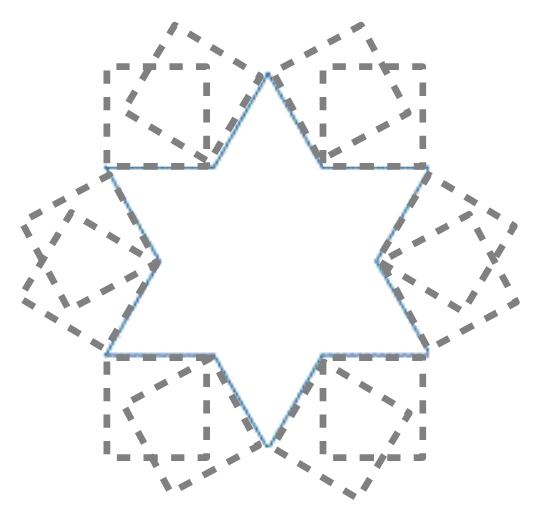
\includegraphics[height=2.5cm]{koch_1.png} & $\rightarrow$ & 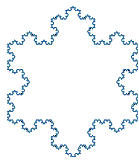
\includegraphics[height=2.5cm]{koch_k.png}\\
$K^{(0)}$ & & $K^{(1)}$ & ... & $K^{(k)}$\\
1 seul carré & & 12 carrés & ... & $3\times 4^k$ carrés\\
de côté 1 & & de côté $\frac{1}{3}$ & ... & de côté $\varepsilon_k = \frac{1}{3^k}$\\
\end{tabular} \\ \\ \\
Donc $d=\lim\limits_{k \rightarrow \infty} 3\times \frac{ln(4^k)}{ln(3^k)}=3\times \frac{ln(4)}{ln(3)}=3\times \frac{2ln(2)}{ln(3)}$ est la dimension de Hausdorff.\\ \\
On peut restreindre l'étude du flocon de Von Koch à l'étude de la courbe de Von Koch (figure \ref{courbe_vonkoch}). L'algorithme de construction est le même à l'exception que la figure de départ est un segment et non un triangle. On a alors $d=\frac{2ln(2)}{ln(3)}$.
\begin{figure}[H]
\caption{Courbe de Von Koch}
\label{courbe_vonkoch}
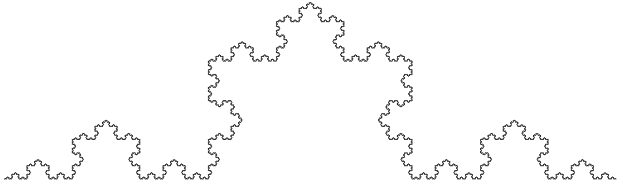
\includegraphics[width=\textwidth]{koch_courbe.png}
\end{figure}

Dans nos applications dans \textit{Scilab}, on se contentera de tracer la courbe de Von Koch. \\ \\

\subsection{Application dans \textit{Scilab} (méthode récursive)}
En s'insipirant toujours de la définition de la fractale, on implémente dans \textit{Scilab} le code \ref{code_koch}.
\begin{table}[H]
\caption{Courbe de Von Koch (méthode récursive)}
\begin{tabular}{l}
\lstinputlisting[language=scilab]{koch_recursif.sce}\\
\end{tabular}
\label{code_koch}
\end{table}
\newpage
L'exécution du code nous donne ainsi la figure \ref{koch_recursif}.
\begin{figure}[H]
\centering
\caption{Figure pour n=4}
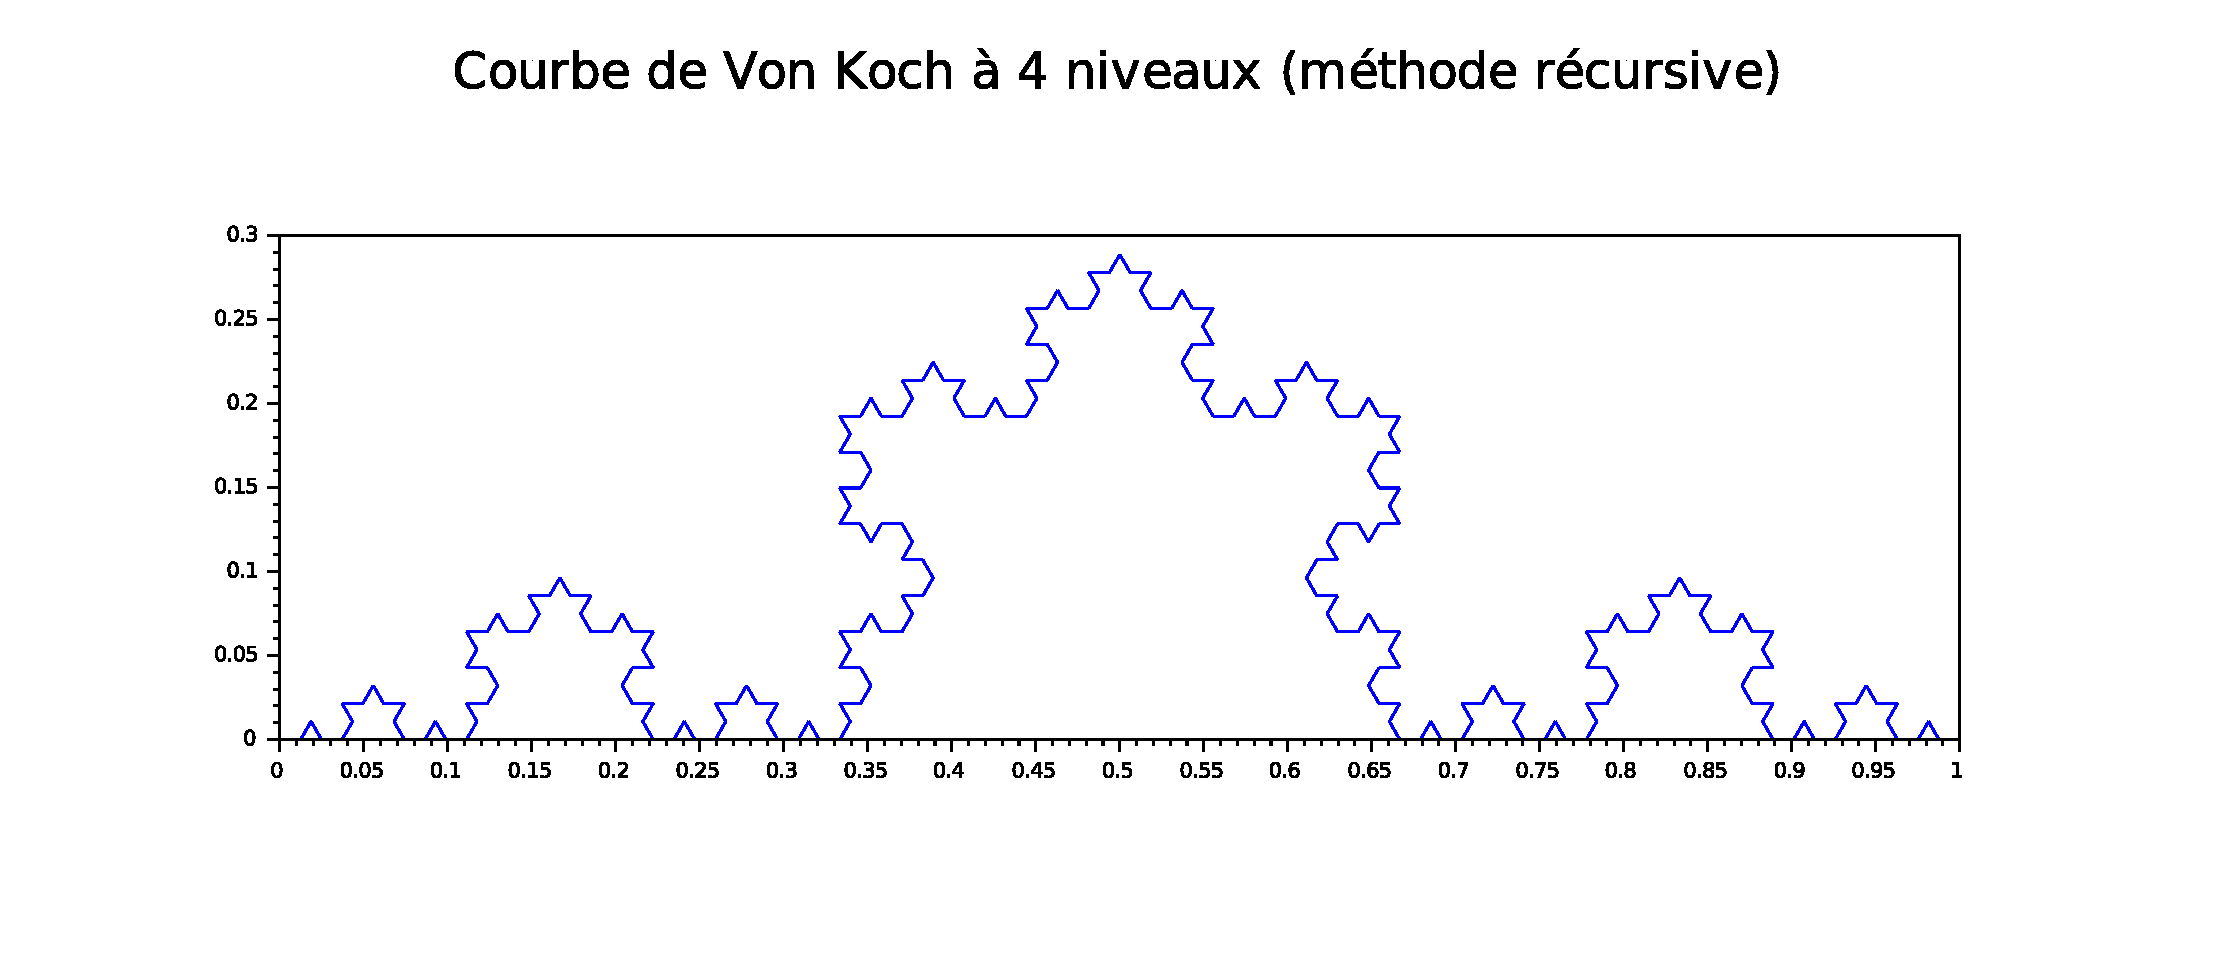
\includegraphics[width=\textwidth]{koch_recursif.pdf}
\label{koch_recursif}
\end{figure}

\subsection{Application dans \textit{Scilab} (méthode itérative)}
La complexité de l'algorithme récursif est ici en $O(4^n)$ (on réalise 4 appels récursifs pour chaque niveau). L'éxecution devient donc très rapidement problématique. Pour des valeurs de $n$ importantes, cette méthode n'est plus applicable. On implémente donc également une méthode itérative à l'aide d'un IFS. On a donc :
\begin{equation}
\left\lbrace
\begin{array}{l}
f_1 \left[ \begin{array}{l} x \\ y \end{array} \right] =
\left[ \begin{array}{ll} \frac{1}{3} & 0 \\ 0 & \frac{1}{3} \end{array} \right]
\left[ \begin{array}{l} x \\ y \end{array} \right]\\ \\

f_2 \left[ \begin{array}{l} x \\ y \end{array} \right] =
\left[ \begin{array}{ll} \frac{1}{6} & -\frac{\sqrt{3}}{6} \\ \frac{\sqrt{3}}{6} & \frac{1}{6} \end{array} \right]
\left[ \begin{array}{ll} x \\ y \end{array} \right]
+ \left[ \begin{array}{l} \frac{1}{3} \\ 0 \end{array} \right]\\ \\

f_3 \left[ \begin{array}{l} x \\ y \end{array} \right] \longrightarrow
\left[ \begin{array}{ll} \frac{1}{6} & \frac{\sqrt{3}}{6} \\ -\frac{\sqrt{3}}{6} & \frac{1}{6} \end{array} \right]
\left[ \begin{array}{ll} x \\ y \end{array} \right]
+ \left[ \begin{array}{l} \frac{1}{2} \\ \frac{\sqrt{3}}{6} \end{array} \right]\\ \\

f_4 \left[ \begin{array}{l} x \\ y \end{array} \right] \longrightarrow
\left[ \begin{array}{ll} \frac{1}{3} & 0 \\ 0 & \frac{1}{3} \end{array} \right]
\left[ \begin{array}{ll} x \\ y \end{array} \right]
+ \left[ \begin{array}{l} \frac{2}{3} \\ 0 \end{array} \right]\\
\end{array}\right.
\end{equation}
$d'o\grave{u} \
\left\lbrace
\begin{array}{l}
K_0 \ donn\acute{e} \\
K_{n+1} = K(T_n) \ avec \ K(T)=f_0(T)\cup f_1(T)\cup f_2(T)\cup f_3(T)\cup f_4(T)\\
\end{array}\right.$\\ \\
Finalement $K_n$ converge au sens de la distance de Hausdorff vers $K^\infty$, le flocon de Von Koch. A nouveau, la dispersion des points doit être uniforme, on utilise donc des conditions d'équiprobabilité. \\ \\

\indent On implémente donc dans \textit{Scilab} le code \ref{code_koch_it}.
\begin{table}[H]
\caption{Flocon de Von Koch (méthode itérative)}
\begin{tabular}{l}
\lstinputlisting[language=scilab]{koch_iteratif.sce}\\
\end{tabular}
\label{code_koch_it}
\end{table}

L'exécution du code nous donne ainsi la figure \ref{koch_iteratif}.
\begin{figure}[H]
\centering
\caption{Flocon de Von Koch itératif pour 10000 points}
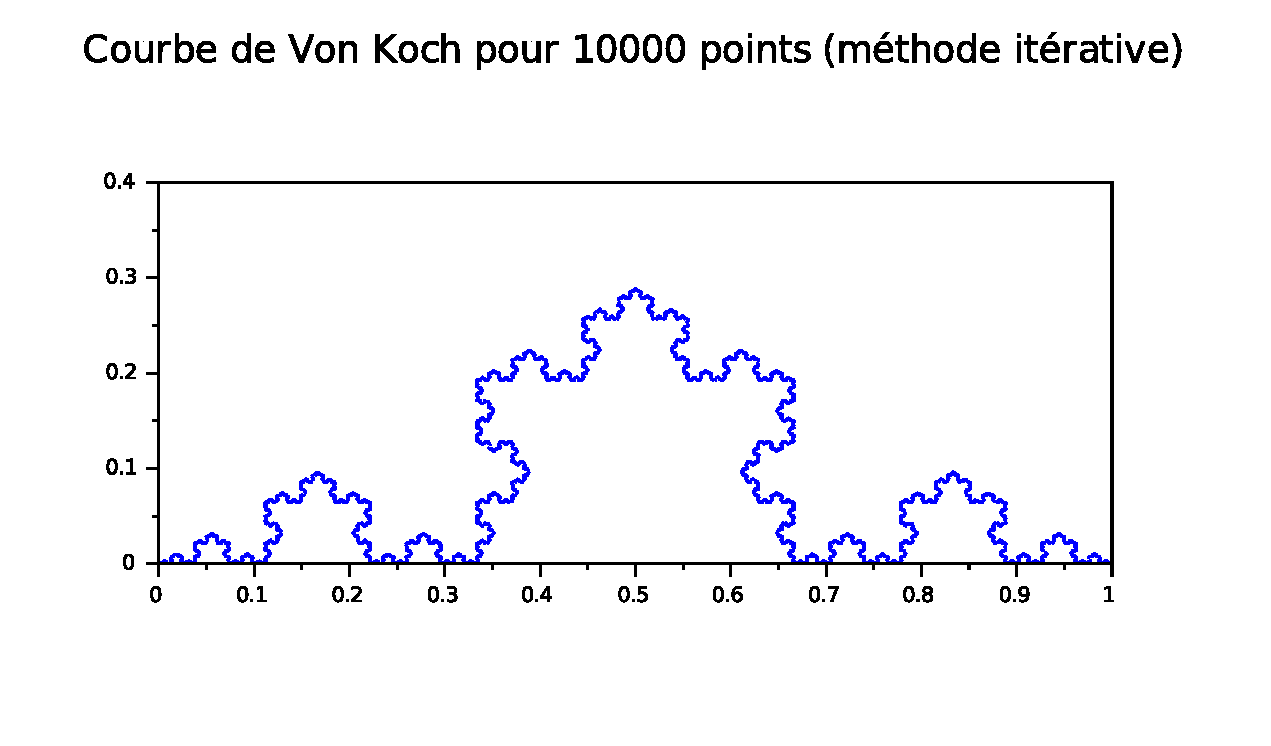
\includegraphics[width=\textwidth]{koch_iteratif.pdf}
\label{koch_iteratif}
\end{figure}

\newpage
\section{Fougère de Barnsley}
\subsection{Théorie}
\subsubsection{Présentation}
\begin{minipage}[c]{.70\linewidth}
	\indent Pour compléter notre étude sur la théorie des IFS, on va s'intéresser à un objet qu'il est impossible de construire de manière récursive : la \textit{fougère de Barnsley}, construite par Michael Barnsley, mathématicien britannique. \\ \\
	On a précédemment vu trois applications de la méthode des IFS avec à chaque fois une dispersion des points de manière uniforme. Il apparaît donc pertinent de s'intéresser à une fractale nécessitant une certaine dispersion des points : \textit{la fougère de Barnsley}.
\end{minipage} \hfill
\begin{minipage}[c]{.05\linewidth}
\end{minipage} \hfill
\begin{minipage}[c]{.21\linewidth}
	\begin{figure}[H]
	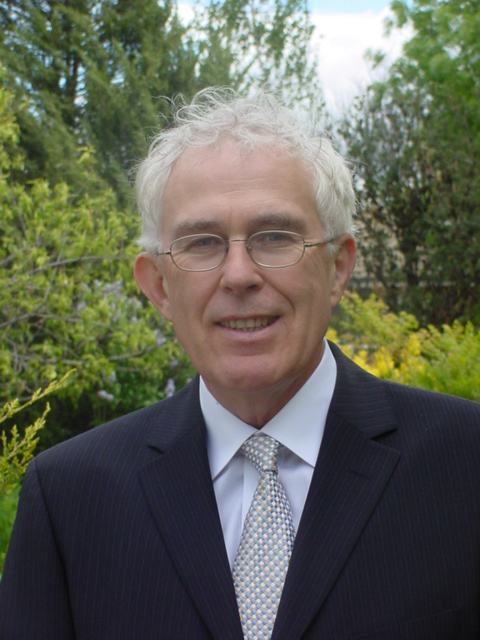
\includegraphics[height=4cm]{mr_barnsley.jpg}
	\caption{Barnsley 1946-...}
	\end{figure}
\end{minipage}

\begin{figure}[H]
\centering
\caption{Fougère de Barnsley}
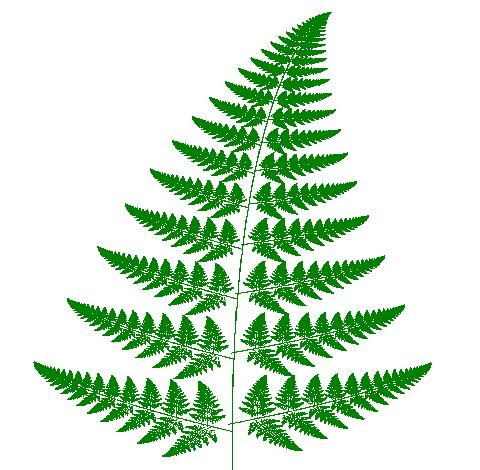
\includegraphics[width=5.5cm]{barnsley.jpg}
\end{figure}

\subsubsection{Définition}
Le système de fonctions itérées est le suivant :
\begin{equation}
\left\lbrace
\begin{array}{l}
f_1\left[ \begin{array}{c} x \\ y \end{array} \right]\ = \ \left[ \begin{array}{cc} 0,00 & 0,00 \\ 0,00 & 0,16 \end{array} \right] \left[ \begin{array}{c} x \\ y \end{array} \right]\\
\\
f_2\left[ \begin{array}{c} x \\ y \end{array} \right]\ = \ \left[ \begin{array}{cc} 0,85 & 0,04 \\ -0,04 & 0,85 \end{array} \right] \left[ \begin{array}{c} x \\ y \end{array} \right] + \left[ \begin{array}{l} 0 \\ 1,6 \end{array} \right] \\
\\
f_3\left[ \begin{array}{c} x \\ y \end{array} \right]\ = \ \left[ \begin{array}{cc} 0,20 & -0,26 \\ 0,23 & 0,22 \end{array} \right] \left[ \begin{array}{c} x \\ y \end{array} \right] + \left[ \begin{array}{l} 0 \\ 1,6 \end{array} \right] \\
\\
f_3\left[ \begin{array}{c} x \\ y \end{array} \right]\ = \ \left[ \begin{array}{cc} 0,15 & 0,28 \\ 0,26 & 0,24 \end{array} \right] \left[ \begin{array}{c} x \\ y \end{array} \right] + \left[ \begin{array}{l} 0 \\ 0,44 \end{array} \right] \\
\end{array}\right.
\end{equation}
Ces fonctions sont responsables de la modélisation de chacune des parties de la fougère. Pour obtenir un dessin réaliste, il est donc nécessaire de privilégier certaines parties par rapport à d'autres (plus la partie gauche que le reste par exemple). \\
Il est conseillé de choisir les pondérations $p_i$ suivantes pour chacune des fonctions $f_i$ :
$p = \left[ \begin{array}{l} 0,01 \\ 0,85 \\ 0,07 \\ 0,07 \end{array} \right]$

\newpage
\subsection{Application dans \textit{Scilab}}
On implémente donc dans \textit{Scilab} le code \ref{code_fougere}.

\begin{table}[H]
\caption{Fougère de Barnsley}
\begin{tabular}{l}
\lstinputlisting[language=scilab]{fougere.sce}\\
\end{tabular}
\label{code_fougere}
\end{table}

L'exécution du code nous donne ainsi la figure \ref{affichage_fougere} pour différentes valeurs de $N$.
\begin{figure}[H]
\caption{Différents affichages de la fougère en fonction de $N$}
   \begin{minipage}[c]{.49\linewidth}
   \centering
      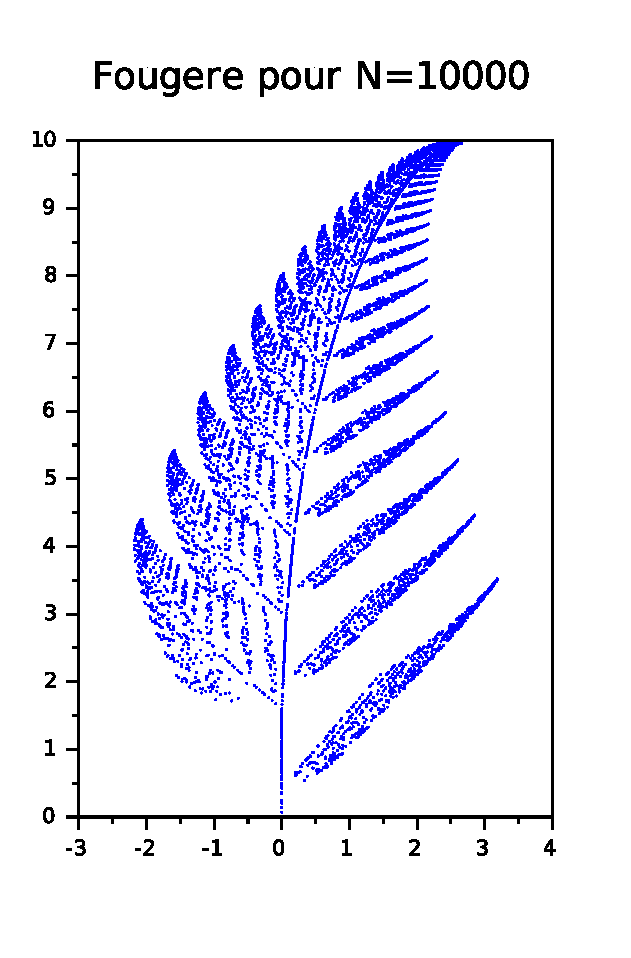
\includegraphics[height=8cm]{graphfougere.pdf}
   \end{minipage} \hfill
   \begin{minipage}[c]{.49\linewidth}
   \centering
      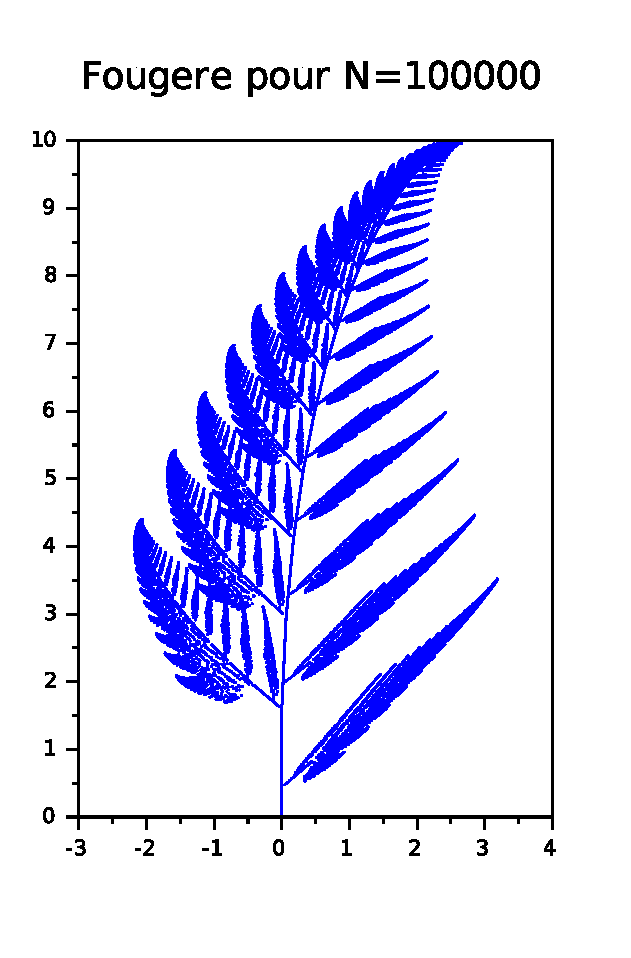
\includegraphics[height=8cm]{graphfougere_2.pdf}
   \end{minipage}
\label{affichage_fougere}
\end{figure}

\section{Ensemble de Julia}

\subsection{Théorie}
\subsubsection{Présentation}
\begin{minipage}[c]{.70\linewidth}
	\indent Nous allons maintenant nous intéresser à des fractales dont la construction est beaucoup moins immédiate que les précédentes (fractales dont on pouvait rapidement représenter quelques itérations, même avec un crayon et une feuille de papier). \\ \\
	La première de ces fractales \textit{plus compliquées} s'appelle l'ensemble de Julia, construite par Gaston Julia, un mathématicien français. Il est à noter que la figure \ref{julia} n'est pas représentative de l'ensemble de Julia : ce dernier peut prendre des formes très différentes selon la modélisation choisie et surtout selon la valeur de $c$. 
\end{minipage} \hfill
\begin{minipage}[c]{.05\linewidth}
\end{minipage} \hfill
\begin{minipage}[c]{.21\linewidth}
	\begin{figure}[H]
	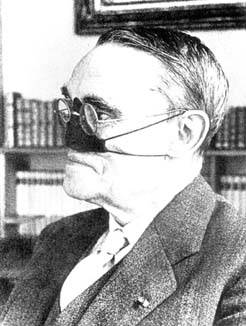
\includegraphics[height=4cm]{mr_julia.jpg}
	\caption{Julia 1893-1978}
	\end{figure}
\end{minipage}

\begin{figure}[H]
\centering
\caption{Ensemble de Julia (exemple parmi beaucoup d'autres)}
\label{julia}
\centering
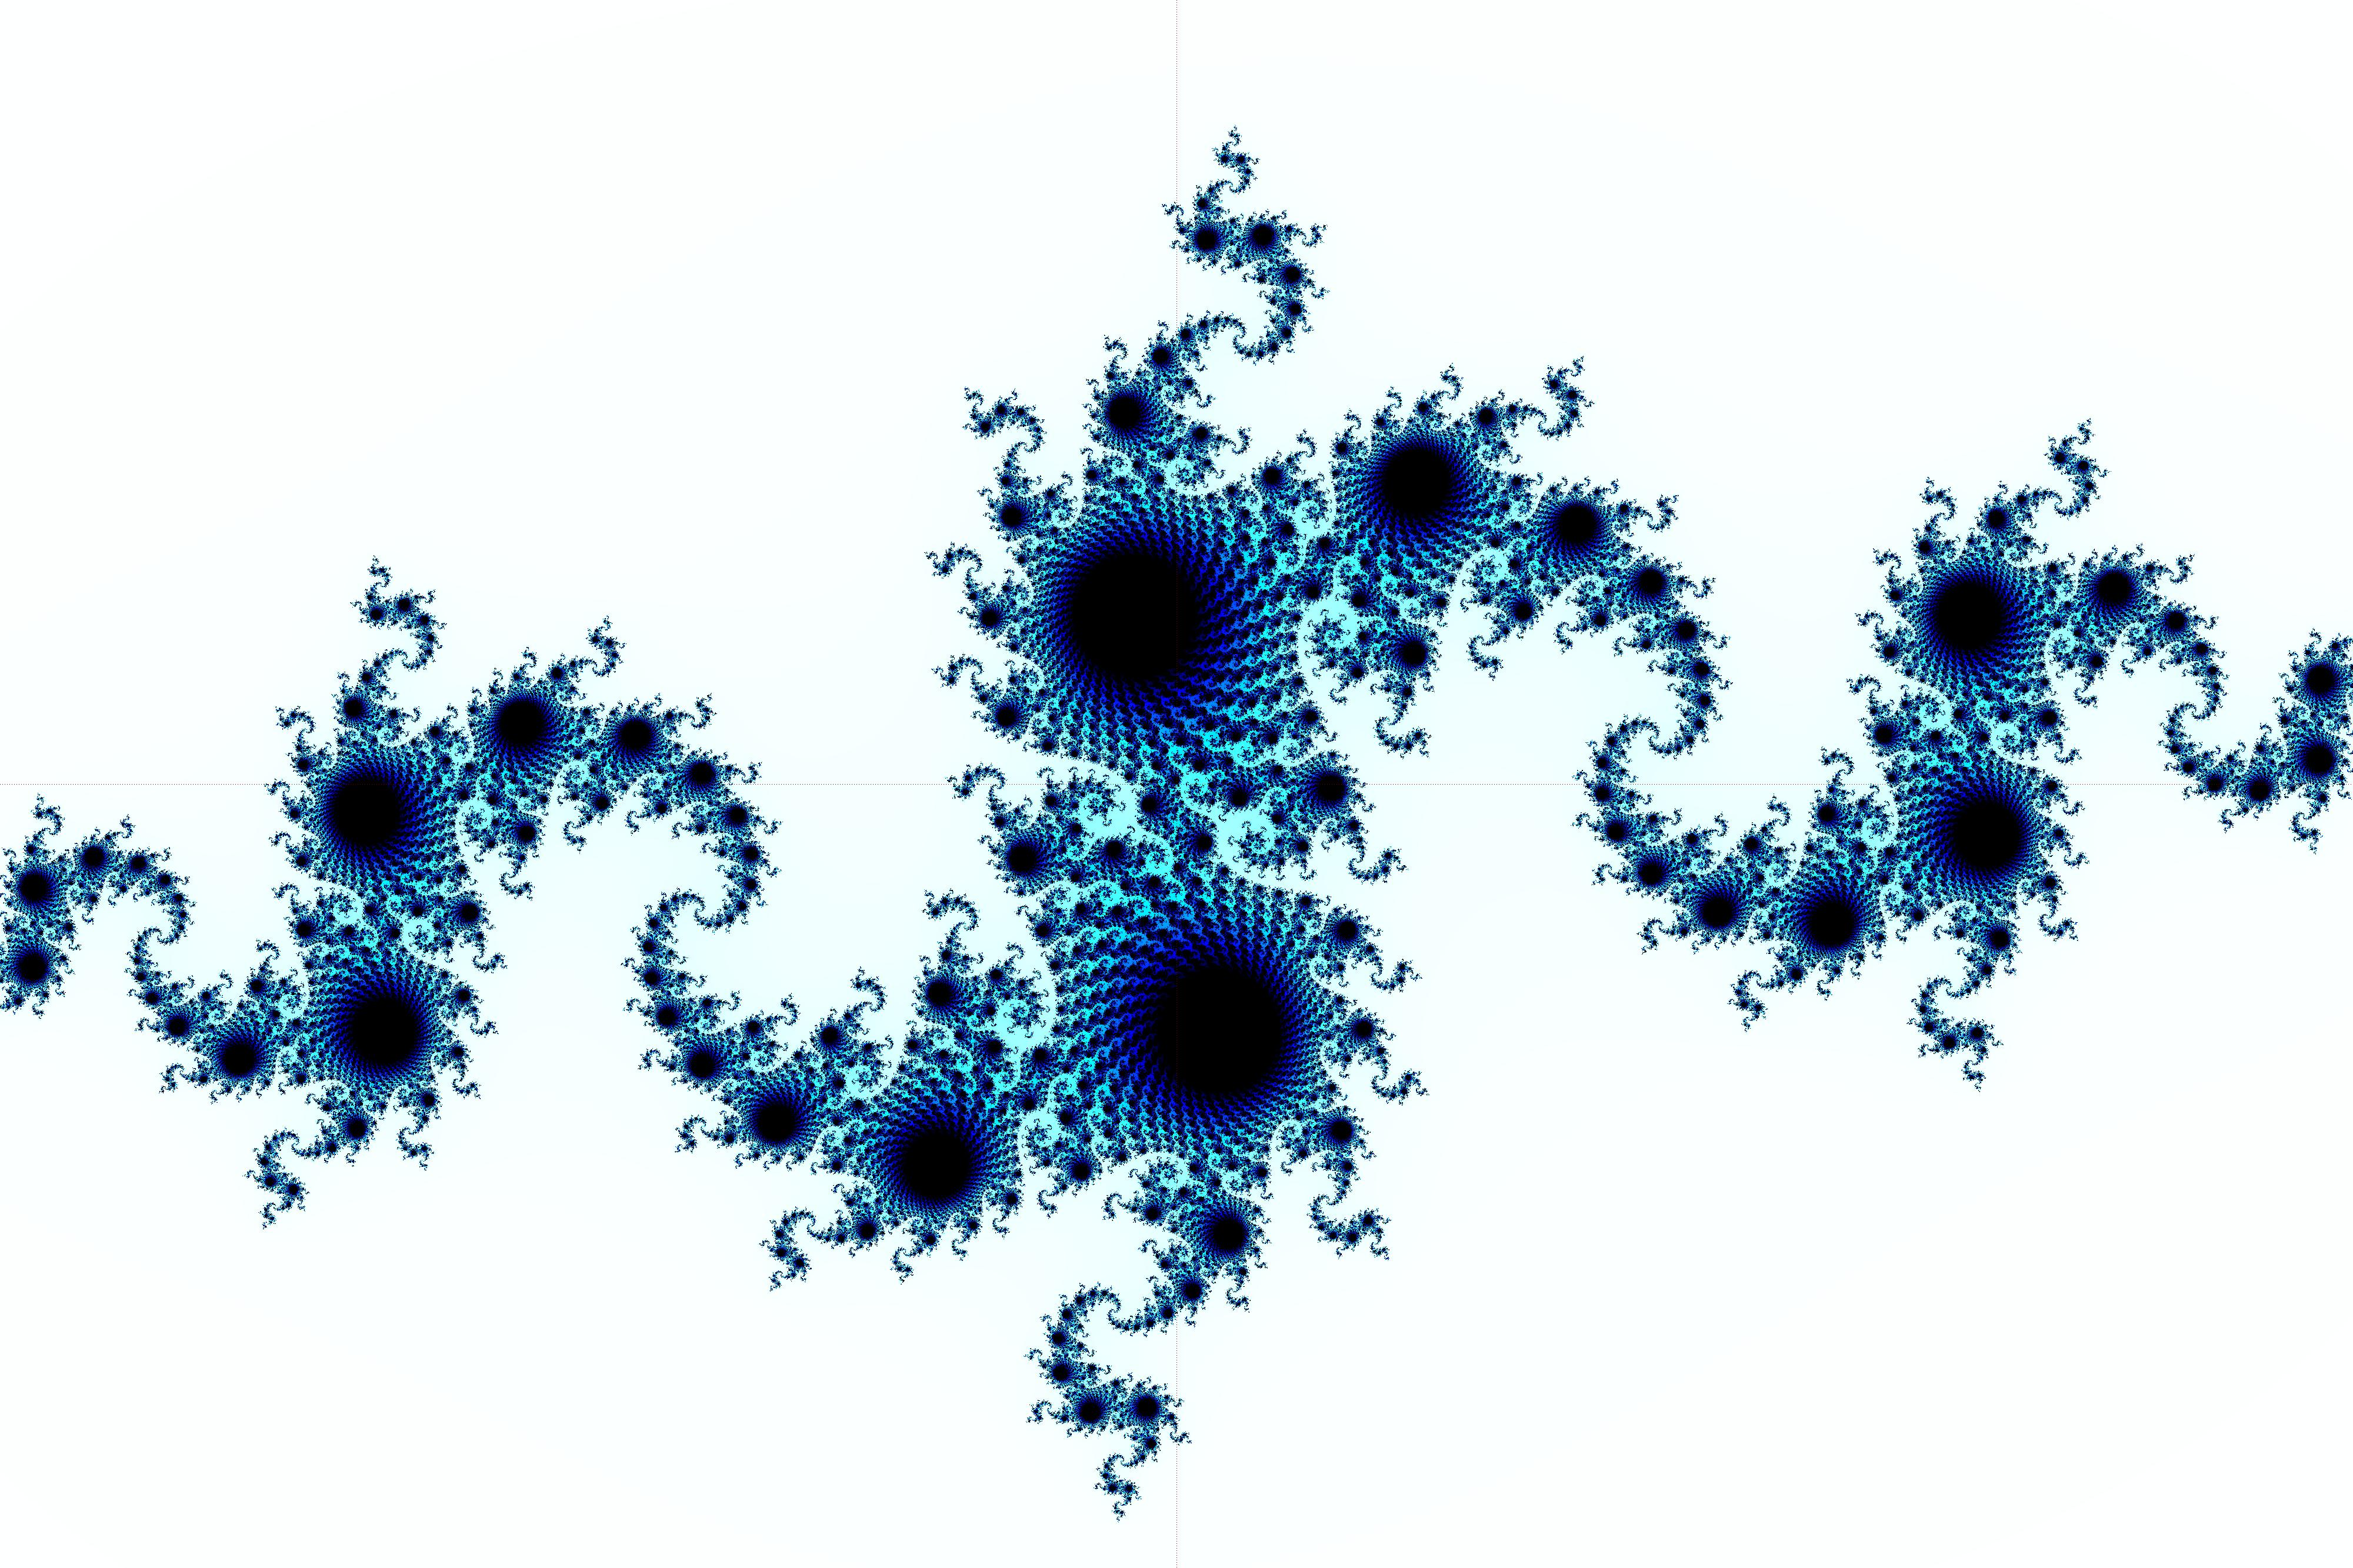
\includegraphics[width=14cm]{julia.jpg}
\end{figure}

\subsubsection{Définition}
On se donne un nombre complexe $c=a+ib$ avec $a,b\ \in \ \mathbb{R}$. On considère alors la suite :
\begin{equation}
\label{suite_julia}
\left\lbrace
\begin{array}{l}
z_{n+1}=z_n^2+c \\
z_0 \ \in \ \mathbb{C}
\end{array}\right.
\end{equation}
On appelle \textit{bassin d'attraction} l'ensemble des points $z_0$ tels que la suite définie en (\ref{suite_julia}) converge, et \textit{bassin de répulsion} l'ensemble des points $z_0$ tels que la suite diverge. L'ensemble de Julia est alors la frontière entre ces deux bassins. L'ensemble de Julia est alors défini en fonction de $c$, qui en devient un paramètre capital. Le choix de $c$ est classique et on peut trouver beaucoup de documentation en ligne sur les valeurs intéressantes à donner à cette variable. En outre, nous verrons un peu plus tard que ces valeurs ne sont pas le fruit du hasard.

\subsection{Application dans \textit{Scilab}}
On implémente donc dans \textit{Scilab} le code \ref{code_julia}.

\begin{table}[H]
\caption{Ensemble de Julia}
\begin{tabular}{l}
\lstinputlisting[language=scilab]{julia.sce}\\
\end{tabular}
\label{code_julia}
\end{table}

L'exécution du code nous donne ainsi la figure \ref{affichage_julia} pour différentes valeurs de $c$.
\begin{figure}[H]
\caption{Différents affichages de l'ensemble de Julia en fonction de $c$}
   \begin{minipage}[c]{.49\linewidth}
   \centering
      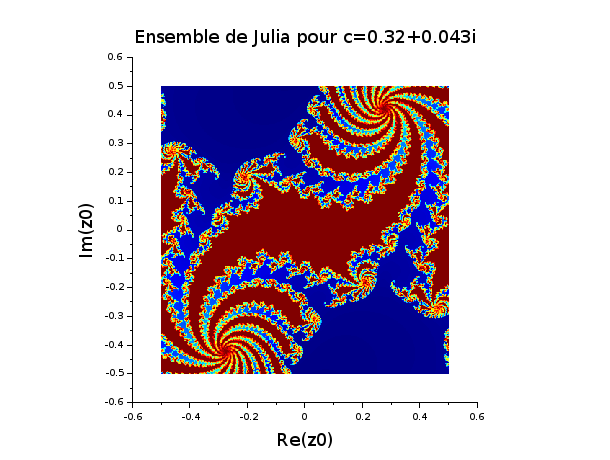
\includegraphics[height=6.5cm]{julia1.png}
      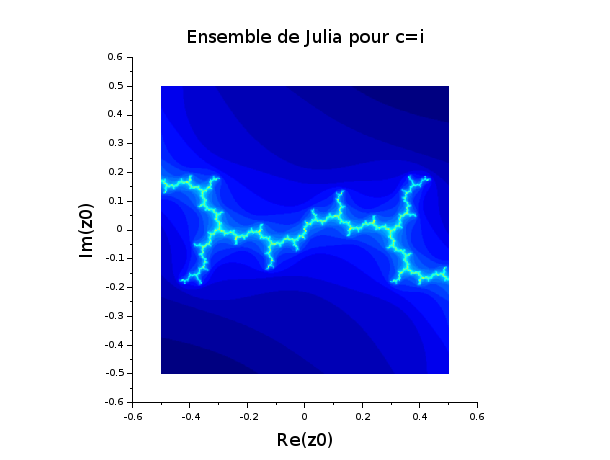
\includegraphics[height=6.5cm]{julia2.png}
   \end{minipage} \hfill
   \begin{minipage}[c]{.49\linewidth}
   \centering
      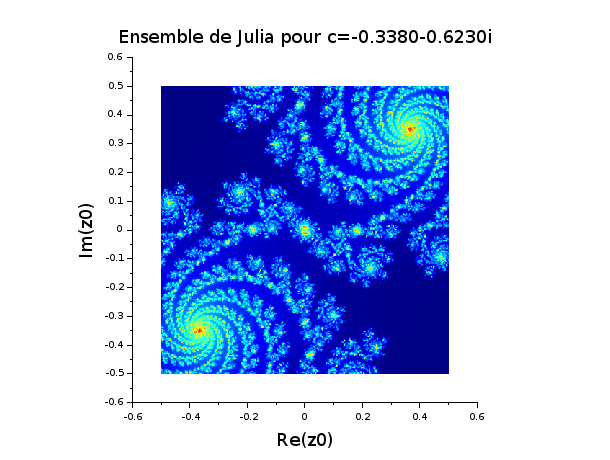
\includegraphics[height=6.5cm]{julia3.png}
      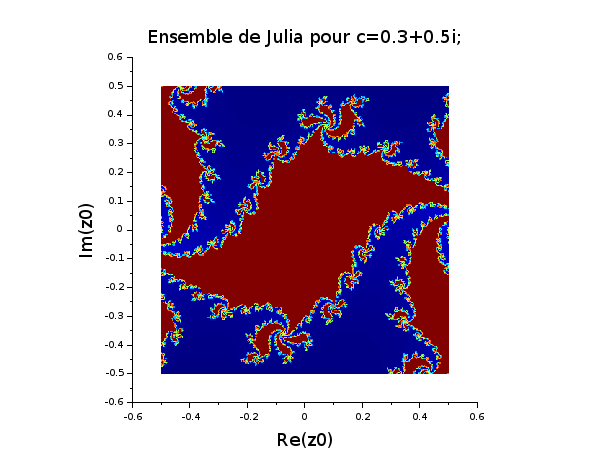
\includegraphics[height=6.5cm]{julia4.png}
   \end{minipage}
\label{affichage_julia}
\end{figure}


\section{Ensemble de Mandelbrot}
\subsection{Théorie}
\subsubsection{Présentation}
Avec l'ensemble de Julia, nous avions vu que la sélection d'une valeur de $c$ \textit{intéressante} était primordiale à la construction de la fractale. \\ \\
\begin{minipage}[c]{.70\linewidth}
	Ainsi la fractale que nous sommes sur le point d'étudier nous permet une représentation de ces valeurs de $c$ en fonction de leur \textit{intérêt}. Il s'agit donc de la fractale nommée \textit{l'ensemble de Mandelbrot}, construite par Benoît Mandelbrot, mathématicien franco-américain.
\begin{figure}[H]
\centering
\caption{Ensemble de Mandelbrot}
\label{julia}
\centering
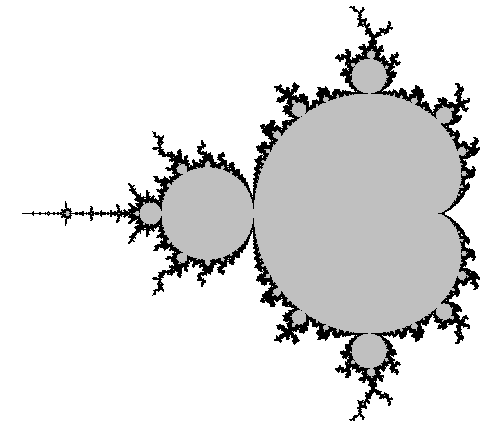
\includegraphics[width=6cm]{mandelbrot.png}
\end{figure}	
\end{minipage} \hfill
\begin{minipage}[c]{.05\linewidth}
\end{minipage} \hfill
\begin{minipage}[c]{.21\linewidth}
	\begin{figure}[H]
	\includegraphics[height=4cm]{mr_mandelbrot.jpg}
	\caption{Mandelbrot 1924-2010}
	\end{figure}
\end{minipage}

\subsubsection{Définition}
La définition de l'ensemble de Mandelbrot est donc largement similaire à celle de l'ensemble de Julia, à la seule différence prés que la valeur de $z_0$ est donnée et que $c$ est une variable.

\subsection{Application dans \textit{Scilab}}
On implémente donc dans \textit{Scilab} le code \ref{code_mandelbrot}.

\begin{table}[H]
\caption{Ensemble de Mandelbrot}
\begin{tabular}{l}
\lstinputlisting[language=scilab]{mandelbrot.sce}\\
\end{tabular}
\label{code_mandelbrot}
\end{table}

L'exécution du code nous donne ainsi la figure \ref{affichage_mandelbrot}.
\begin{figure}[H]
\caption{Ensemble de Mandelbrot}
\centering
\includegraphics[height=8cm]{mandelbrot1.png}
\label{affichage_mandelbrot}
\end{figure}
Ainsi, en construisant les ensembles de Julia associés aux $c$ \textit{intéressants} (dans la limite entre les zones rouge et bleue), on obtient une figure connexe.\\
\indent En effet, on peut comparer les affichages de la figure \ref{affichage_julia_cf_mandelbrot}.

\begin{figure}[H]
\caption{Différents affichages de l'ensemble de Julia en fonction de $c$ (dans ou hors la frontière de Mandelbrot)}
   \begin{minipage}[c]{.49\linewidth}
   \centering
      \includegraphics[height=5.5cm]{julia1_cfM.png}
      \includegraphics[height=5.5cm]{julia2_cfM.png}
   \end{minipage} \hfill
   \begin{minipage}[c]{.49\linewidth}
   \centering
      \includegraphics[height=5.5cm]{julia3_cfM.png}
      \includegraphics[height=5.5cm]{julia4_cfM.png}
   \end{minipage}
\label{affichage_julia_cf_mandelbrot}
\end{figure}

\chapter{Équations différentielles}
\section{Introduction}
Dans de très nombreux domaines comme la mécanique, la biologie, la chimie ou encore l'économie, beaucoup de problèmes font appel à des équations différentielles. On est ainsi souvent confronté à ce que l'on appelle des \textit{problème de Cauchy} sous la forme suivante :\\
\begin{equation}
\label{equa_diff}
\left\lbrace
\begin{array}{l}
y^{(m)}=h(t,y,y',\cdots ,y^{(m-1)}) \\
y(0)=a_0 \\
y'(0)=a_1 \\
\cdots \\
y^{(m-1)}(0)=a_{m-1} \\
\end{array}\right.
\end{equation}

Pour résoudre (\ref{equa_diff}), on se ramène alors à un système différentiel d'ordre 1 :
\begin{equation}
\begin{array}{llllll}
Y= &
\left(
\begin{array}{l}
y_1 \ (la \ solution) \\
y_2=y'_1 \\
\vdots \\
y_m=f(t,y_1,y_2,\cdots ,y_{m-1}) \\
\end{array}\right)

& &
Y(0)= &
\left(
\begin{array}{c}
a_0 \\
a_1 \\
\vdots \\
a_{m-1} \\
\end{array}\right) \in \textbf{R}^m \\ \\
donc &
\left\lbrace
\begin{array}{l}
Y'=F(t,Y) \\
y(0)=(a_0,\cdots ,a_{m-1})^T \\
\end{array}\right.
& avec & F(t,Y)= &
\left(
\begin{array}{c}
y_1\\
y_2\\
\vdots \\
y_{m-1} \\
f(t,y_1,y_2,\cdots ,y_{m-1})
\end{array}\right)
\end{array}
\end{equation}
\\

\indent Cependant, considérons le problème suivant :
\begin{equation}
\label{equa_diff_pb}
\left\lbrace
\begin{array}{l}
y'=e^{-t^2}y \\
y(0)=1
\end{array}\right.
\end{equation}
on a (\ref{equa_diff_pb}) $\Rightarrow \ \frac{dy}{dt} = e^{-t^2}y \ \Rightarrow \ \frac{dy}{y} = e^{-t^2}dt \ \Rightarrow \ \int_{}^{} \frac{dy}{y} = \int_{}^{} e^{-t^2}dt \ \Rightarrow \ ln(y) = \int_{}^{} e^{-t^2}dt $\\
Or on ne connaît pas de primitive de $t \longrightarrow e^{-t^2}$, on ne peut donc pas résoudre le système (\ref{equa_diff_pb}) de manière analytique. Dans ce genre de situation, on a alors recours à un schéma numérique.

\newpage
\section{Idée, stabilité, consistance et ordre d'un schéma numérique}
\subsection{Idée}
L'idée générale d'un schéma numérique est la suivante :\\
On crée une subdivision de l'intervalle d'étude $[t_0,t_0+T]$.\\
On obtient donc $\sigma = \left\lbrace t_0,t_1,\cdots ,t_N \right\rbrace$ avec $t_N=t_0+N$.\\
On note le pas de la subdivision $h=\underset{0\leq i \leq N}{max} |t_{i+1}-t_i|$.\\
On se placera toujours dans la cas d'une substitution \textit{uniforme} : $h_i=|t_{i+1}-t_i|=h \ \ \ \forall i$\\
L'idée est alors d'approcher $y(t_i)$ par $z_i$ où :
\begin{equation}
\left\lbrace
\begin{array}{l}
z_{i+1}=z_i+h\Phi (t_i,z_i,h) \\
z_0=y_0
\end{array}\right.
\end{equation}\\
Chacune de ces approximations sera alors appelée un \textit{schéma}. Un schéma donné a différentes propriétés remarquables : une stabilité, une consistance et un ordre.

\subsection{Stabilité d'un schéma numérique}
\subsubsection{Définition}
soit $(u_i)$ et $(v_i)$ telle que :\\
$\left\lbrace
\begin{array}{l}
u_{i+1}=u_i+h\Phi (t_i,u_i,h) \\
u(0) \text{ donné}
\end{array}\right.$
et  
$\ \left\lbrace
\begin{array}{l}
v_{i+1}=v_i+h\Phi (t_i,v_i,h) + \xi _i \\
v(0) \text{ donné}
\end{array}\right.
\ \ \ \forall i=0,\cdots , N-1$ \\
$\textbf{Le schéma est stable} \text{ si } \ \underset{0\leq i \leq N-1}{max} |u_i-v_i|\leq C \left( |u_0-v_0|+\sum \limits_{i=1}^N |\xi _i| \right)$\\
où $C$ est une constante ne dépendant pas de $(u_i)$ et $(v_i)$.

\subsubsection{Théorème}
\abovedisplayskip=0mm
\begin{align*}
   \text{Le schéma est stable} & \Leftrightarrow \exists K>0, \ ||\Phi(t,y,h)-\Phi(t,z,h)||\leq K||Y-Z|| \\
							   & \Leftrightarrow \Phi \text{ est } K-lipschitzienne \text{ par rapport à la deuxième variable}
\end{align*} 

\subsection{Consistance d'un schéma numérique}
\subsubsection{Définition}
$\textbf{Le schéma est consistant} \text{ si } \xi(y)=\sum ||y-t_{i+1}-y(t_i)-\Phi(t_i,y(t_i),h)|| \underset{h\rightarrow 0}{\longrightarrow} 0$\\
ou d'une manière équivalente : si $\Phi(t,y,0)=f(t,y)$

\subsection{Ordre d'un schéma numérique}
\subsubsection{Définition}
$\textbf{Le schéma est d'ordre p} \text{ si } \exists C > 0, \ \underset{1\leq i \leq N}{max} |y(t_i)-z_i| \leq Ch^p $

\subsubsection{Autre définition}
$\textbf{Le schéma est d'ordre p} \text{ si l'erreur de consistance locale } T_i = \frac{y(t_{i+1}-y(t_i)}{h}- \Phi(t,y(t_i),h)$\\
$\text{ est telle que } |T_i|\leq Ch^p$

\newpage
\section{Schéma d'Euler}
\subsection{Théorie}
\subsubsection{Définition}
\begin{minipage}{.41\linewidth}
\includegraphics[width=\textwidth]{rectangle.png}
\end{minipage} \hfill
\begin{minipage}{.05\linewidth}
\end{minipage} \hfill
\begin{minipage}{.53\linewidth}
\noindent Le théorème fondamental de l'analyse nous donne : $y(t_{i+1}) = y(t_i) + \int_{t_i}^{t_{i+1}} y'dt = y(t_i) + \int_{t_i}^{t_{i+1}} f(t,y(t))dt$\\
La valeur de $\int_{t_i}^{t_{i+1}} f(t,y(t))dt$ est inconnue, il faut donc l'approcher.\\ \\
On l'approche par \textbf{l'aire du rectangle gauche} :
\abovedisplayskip=0mm
\begin{align*}
   y(t_{i+1}) & \thicksim y(t_i)+ \text{Aire du rectangle gauche} \\
			  & \thicksim y(t_i)+ hf(t_i,y(t_i))
\end{align*}
D'où \textbf{le schéma d'Euler} :
\begin{equation}
\left\lbrace
\begin{array}{l}
z_{i+1}=z_i+hf(t_i,z_i) \\
z_0 \text{ donné, } z_0=y_0
\end{array}\right.
\end{equation}
\end{minipage}

\subsubsection{Propriétés}
\noindent Le schéma d'Euler est \textbf{stable}, \textbf{consistant} et \textbf{d'ordre 1} (si $f$ est L-lipschitzienne par rapport à la $2^{\text{ème}}$ variable).  \\

\textbf{Démo (stabilité) :}\\
\indent On pose $\Phi(t,y,h)=f(t,y)$, ainsi $||\Phi(t,y,h)-\Phi(t,z,h)|| = ||f(t,y)-f(t,z)||$\\
\indent On a $f$ L-lipschitzienne par rapport à la $2^{\text{ème}}$ variable, alors $||f(t,y)-f(t,z)||\leq L||y-z||$\\

\textbf{Démo (consistance) :}\\
\indent On pose $\Phi(t,y,h)=f(t,y)$ $\forall h$ donc on a en particulier $\Phi(t,y,0)=f(t,y)$\\

\textbf{Démo (ordre) :}\\
\indent On a $\left\{\begin{array}{l}y_{i+1}=y_i+hf(t_i,y_i)  \\
		y(t_{i+1})=y(t_i+h)\ \overset{Taylor-Lagrange}{=}\ y(t_i)+h\underbrace{y'(t_i)}_{f(t_i,y_i)}+\frac{h^2}{2}y''(\underbrace{\xi_i}			_{\xi_i\in(t_i,t_{i+1})})\end{array} \right.$\\
\indent d'où $||y(t_{i+1})-y_{i+1}||=(y(t_i)-y_i)+h[f(t_i,y(t_i))-f(t_i,y_i)]+\frac{h^2}{2}y''(\xi_i)$.\\
\indent On a $f$ L-lipschitzienne par rapport à la $2^{\text{ème}}$ variable : $\exists L>0,\ ||f(t,y)-f(t,z)||\leq L||y-z||$.\\
\indent On suppose que $\exists M>0$ tel que $||y''(\xi)||<M,\ \forall\xi\in[t_0,t_0+T]$,\\
\indent d'où, si on note $e_i=y(t_i)-z_i$, on a :
		$$\begin{array}{lll}
		||e_{i+1}||&\leq&\underbrace{(1+hL)}_{C}||e_i||+\underbrace{\frac{h^2}{2}M}_{D}\\
		||e_{i+1}||&\leq&C||e_i||+D\\
				   &\leq&C[C||e_{i-1}||+D]+D=C^2||e_{i-1}||+D(1+C)\\
		           &\leq&C^{i+1}e_0+D[1+C+\cdots+C^{i-1}]=C^ie_0+D\frac{C^i-1}{C-1}
		\end{array}$$
\indent Si $y(t_0)=y_0$ alors $e_0=0$. Donc :
		$$\begin{array}{lll}
		||e_{i+1}||&\leq&\frac{h^2}{2}M\frac{(1+hL)^i-1}{(1+hL)-1}\\
		           &\leq&\frac{h}{2L}M[(1+hL)^i-1]
		\end{array}$$
\indent On utilise $(1+x)^m\leq e^{xm},\ \forall m,\forall x>0$:
		$$\begin{array}{lll}
		||e_{i+1}||&\leq&h\frac{M}{2L}[e^{ihL}-1]=h\frac{M}{2L}[e^{L(t_i-t_0)}]\\
		           &\leq&[\frac{M}{2L}(e^T-1)]h\\
				   &\leq&Ch^{\textcolor{red}{\textcircled{\scriptsize 1}}}
		\end{array}$$

\subsection{Application dans \textit{Scilab}}
Comme exemple d'application des différents schémas, nous allons donc considérer une équation différentielle particulière que nous sommes capable de résoudre analytiquement. Ainsi, nous pourrons comparer la valeur obtenue par approximation avec la solution exacte. On considère ainsi l'équation différentielle (\ref{exemple_equa_diff}).
\begin{equation}
\label{exemple_equa_diff}
\left\lbrace
\begin{array}{l}
y'=-ty+t \ \ \ t \in [0,4] \\
y(0)=0
\end{array}\right.
\end{equation} \\
La résolution analytique du système (\ref{exemple_equa_diff}) est la suivante :\\
\textbf{Solution homogène :} L'équation homogène est donc $y_h'=-ty_h$ qui a pour solution $y_h=Ce^{\frac{-t^2}{2}}$\\
\textbf{Solution particulière :} Par la méthode de la variation de la constante, on a :\\$C'(t)e^{\frac{-t^2}{2}}=t \Rightarrow C'(t)=te^{\frac{t^2}{2} } \Rightarrow C=e^{\frac{t^2}{2} }$ donc $y_p=1$\\
\textbf{Solution générale :} La solution générale est donc $y=y_h+y_p=Ce^{\frac{-t^2}{2}}+1$\\ \\

\indent Nous implémentons le schéma d'Euler afin d'approcher cette solution. On implémente donc dans \textit{Scilab} le code \ref{code_euler}.
\begin{table}[H]
\caption{Schéma d'Euler}
\begin{tabular}{l}
\lstinputlisting[language=scilab]{euler.sce}
\label{code_euler}
\end{tabular}
\end{table}

L'exécution du code \ref{code_euler} nous donne l'affichage (\ref{graph_euler}) (comme commenté dans le code, on réalise deux affichages pour rendre compte au mieux de l'approximation : un affichage large sur l'intervalle $[0;4]$ et un affichage \textit{zoom} sur $[1,8;3]$).
\begin{figure}[H]
\centering
\caption{Affichage (schéma d'Euler)}
\includegraphics[width=\textwidth]{euler.pdf}
\label{graph_euler}
\end{figure}

\section{Schéma du point milieu}
\subsection{Théorie}
\subsubsection{Définition}
\begin{minipage}{.41\linewidth}
\includegraphics[width=\textwidth]{rectangle_milieu.png}
\end{minipage} \hfill
\begin{minipage}{.05\linewidth}
\end{minipage} \hfill
\begin{minipage}{.53\linewidth}
On rappelle que l'on a :\\
$y(t_{i+1}) = y(t_i) + \int_{t_i}^{t_{i+1}} y'dt = y(t_i) + \int_{t_i}^{t_{i+1}} f(t,y(t))dt$\\ \\
On approche $\int_{t_i}^{t_{i+1}} f(t,y(t))dt$ par \textbf{l'aire du rectangle du point milieu} :
\abovedisplayskip=0mm
\begin{align*}
   y(t_{i+1}) & \thicksim y(t_i)+hf\left( t_i+\frac{h}{2}, y\left(t_i+\frac{h}{2}\right)\right) \\
			  & \thicksim y(t_i)+hf\left( t_i+\frac{h}{2}, y(t_i)+\frac{h}{2}f\left(t_i,y(t_i)\right)\right)
\end{align*}
D'où \textbf{le schéma dit du point milieu} :
\begin{equation}
\left\lbrace
\begin{array}{l}
z_{i+1}=z_i+hf\left(t_i+\frac{h}{2},z_i+\frac{h}{2}f(t_i,z_i)\right) \\
z_0 \text{ donné, } z_0=y_0
\end{array}\right.
\end{equation}
\end{minipage}


\subsubsection{Propriétés}
Le schéma du point milieu est \textbf{stable}, \textbf{consistant} et \textbf{d'ordre 2}.\\
(si $f$ est L-lipschitzienne par rapport à la $2^{\text{ème}}$ variable)  \\

\newpage
\textbf{Démo (stabilité) :}\\
\indent On pose $\Phi(t,y,h)=f(t + \frac{h}{2}, y + \frac{h}{2}f(t,y))$, ainsi :
\begin{align*}
||\Phi(t,y,h)-\Phi(t,z,h)|| & = f(t+\frac{h}{2},y+\frac{h}{2}f(t,y)) - f(t+\frac{h}{2},z+\frac{h}{2}f(t,z))  \\
							& \leq L|y+\frac{h}{2}f(t,y)-z-\frac{h}{2}f(t,z)| \\
							& \leq L\left[ |y-z| + \frac{h}{2}|f(y,y)-f(t,z)| \right] \\
							& \leq |y-z|(L+\frac{h}{2}L^2) \\
							& \leq C|y-z|
\end{align*}
\indent Ce qui montre que le schéma du point milieu est stable. \\

\textbf{Démo (consistance) :}\\
\indent On a $\Phi(t,y,0)=f(t,y)$\\
\indent Ce qui montre que le schéma du point milieu est consistant.\\

\textbf{Démo (ordre) :}\\
\indent $T_i =\frac{y(t_{i+1})-y(t_i)}{h}-\Phi(t,y(t_i),h)$\\
\indent On a d'une part :\\
\indent $y(t_{i+1})=y(t_i+h)=y(t_i)+hy'(t_i)+\frac{h^2}{2}y''(t_i)+\frac{h^3}{3!}y^{(3)}(\xi_i)$ pour $t_i<\xi_i<t_{i+1}$
\begin{align*}
\frac{y(t_i+h)-y(t_i)}{h} & = y'(t_i)+\frac{h}{2}y''(t_i)+\frac{h^2}{3!}y^{(3)}(\xi_i) \\
						  & = f(t_i,y(t_i))+\frac{h}{2} \frac{d}{dt}f(t,y(t))|_{t=t_i} + \frac{h^2}{6}y^{(3)}(\xi_i) \\
						  & = f(t_i,y(t_i))+\frac{h}{2}\left[\frac{df}{dt}(t,y(t))+\frac{df}{dy}y'(t)\right]|_{t=t_i} + \frac{h^2}{6}y^{(3)}(\xi_i) \\
						  & = f(t_i,y(t_i))+\frac{h}{2}\left[\frac{df}{dt}(t_i,y(t_i))+\frac{df}{dy}(t_i,y(t_i))\times f(t_i,y(t_i))\right] + \frac{h^2}{6}y^{(3)}(\xi_i)
\end{align*}
\indent On a d'autre part :\\
\begin{align*}
\Phi(t,y(t_i),h) & = f(t_i+\frac{h}{2}, y(t_i)+\frac{h}{2}f(t_i,y(t_i)) \\
				 & = f(t_i,y(t_i))+\frac{h}{2}\left[\frac{df}{dt}(t_i,y(t_i))+\frac{df}{dy}(t_i,y(t_i))\times f(t_i,y(t_i))\right] -O(h^2)
\end{align*}
\indent Donc (on soustrait les deux équations obtenues) :\\
\indent $T_i=\frac{h^2}{6}y^{(3)}(\xi_i) + O(h^2)$ d'où $T_i \leq Ch^{\textcolor{red}{\textcircled{\scriptsize 2}}}$ \\
\indent Ce qui montre que le schéma du point milieu est d'ordre 2.\\ \\

\subsection{Application dans \textit{Scilab}}
On s'intéresse une nouvelle fois à l'équation différentielle (\ref{exemple_equa_diff}), à savoir :\\
\begin{equation*}
\left\lbrace
\begin{array}{l}
y'=-ty+t \ \ \ t \in [0,4] \\
y(0)=0
\end{array}\right.
\end{equation*} \\
Dont on rappelle la solution : $y=Ce^{\frac{-t^2}{2}}+1$\\ \\

On implémente donc dans \textit{Scilab} le schéma du point milieu avec le code \ref{code_pointmilieu} qui nous donne l'affichage (\ref{graph_pointmilieu}).
\begin{table}[H]
\caption{Schéma du point milieu}
\begin{tabular}{l}
\lstinputlisting[language=scilab]{pointmilieu.sce}
\label{code_pointmilieu}
\end{tabular}
\end{table}

\begin{figure}[H]
\centering
\caption{Affichage (schéma du point milieu)}
\includegraphics[width=\textwidth]{point-milieu.pdf}
\label{graph_pointmilieu}
\end{figure}

\section{Schéma d'Euler-Cauchy}
\subsection{Théorie}
\subsubsection{Définition}
\begin{minipage}{.36\linewidth}
\includegraphics[width=\textwidth]{trapeze.png}
\end{minipage} \hfill
\begin{minipage}{.02\linewidth}
\end{minipage} \hfill
\begin{minipage}{.56\linewidth}
On rappelle que l'on a :\\
$y(t_{i+1}) = y(t_i) + \int_{t_i}^{t_{i+1}} y'dt = y(t_i) + \int_{t_i}^{t_{i+1}} f(t,y(t))dt$\\ \\
On approche $\int_{t_i}^{t_{i+1}} f(t,y(t))dt$ par \textbf{l'aire du trapèze} :
\abovedisplayskip=0mm
$y(t_{i+1}) \thicksim y(t_i)+\frac{h}{2} \left[ f(t_i,y(t_i)) + f(t_{i+1},y(t_{i+1})) \right]$ \\
$\thicksim y(t_i)+\frac{h}{2} \left[ f(t_i,y(t_i)) + f(t_i+h,y(t_i)+hf(t_i,y(t_i)) \right]$\\ \\
D'où \textbf{le schéma d'Euler-Cauchy} :\\
\begin{equation}
\left\lbrace
\begin{array}{l}
z_{i+1}=z_i+\frac{h}{2} \left[ f(t_i,z_i) + f(t_i+h,z_i+hf(t_i,z_i) \right] \\
z_0 \text{ donné, } z_0=y_0
\end{array}\right.
\end{equation}
\end{minipage}

\subsubsection{Propriétés}
Le schéma d'Euler-Cauchy est \textbf{stable}, \textbf{consistant} et \textbf{d'ordre 2}.\\
(si $f$ est L-lipschitzienne par rapport à la $2^{\text{ème}}$ variable)  \\

\textbf{Démo (stabilité) :}\\
\indent On pose $\Phi(t,y,h)=\frac{f(t,y)+f(t+h,y+hf(t,y)}{2}$, ainsi :
\begin{align*}
||\Phi(t,y,h)-\Phi(t,z,h)|| & = \frac{1}{2}||f(t,y)-f(t,z)+f(t+h,y+hf(t,y))-f(t+h,z+hf(t,z))|| \\
							& \leq \frac{1}{2}\left[ L|y-z| + L{|y-z|+h(f(t,y)-f(t,z))} \right] \\
							& \leq \frac{1}{2}|y-z|\left[ L + L + hL^2 \right] \\
							& \leq C|y-z|
\end{align*}
\indent Ce qui montre que le schéma d'Euler-Cauchy est stable. \\

\textbf{Démo (consistance) :}\\
\indent On a $\Phi(t,y,0)=\frac{f(t,y)+f(t,y)}{2}=f(t,y)$\\
\indent Ce qui montre que le schéma d'Euler-Cauchy est consistant.\\

\textbf{Démo (ordre) :}\\
\begin{align*}
T_i & =\frac{y(t_{i+1})-y(t_i)}{h}-\Phi(t,y(t_i),h) \\
	& =\frac{y(t_{i+1})-y(t_i)}{h} - \frac{1}{2}(f(t_i,y(t_i))+f(t_i+h,y(t_i)+hf(t_i,y(y_i))) \\
	& = f(t_i,y(t_i))+\frac{h}{2}\left[ \frac{df}{dt}(t_i,y(t_i)) + \frac{df}{dy}f(t_i,y(t_i)) \right] + \frac{h^2}{2}y^{(3)}(\xi_i)\\
	& - \frac{1}{2}(f(t_i,y(t_i))+f(t_i,y(t_i))) + h\frac{df}{dt}(t_i,y(t_i)) + h\frac{df}{dy}f(t_i,y(t_i)) + O(h^2) \\
	& = \frac{h^2}{2}y^{(3)}(\xi_i) + O(h^2)
\end{align*}
\indent Donc $T_i \leq Ch^{\textcolor{red}{\textcircled{\scriptsize 2}}}$ \\
\indent Ce qui montre que le schéma d'Euler-Cauchy est d'ordre 2.\\ \\

\subsection{Application dans \textit{Scilab}}
On s'intéresse toujours à l'équation différentielle (\ref{exemple_equa_diff}), à savoir :\\
\begin{equation*}
\left\lbrace
\begin{array}{lll}
y'=-ty+t \ \ \ t \in [0,4] & \text{    } & \text{solution : }y=Ce^{\frac{-t^2}{2}}+1 \\
y(0)=0
\end{array}\right.
\end{equation*} \\

On implémente donc dans \textit{Scilab} le schéma d'Euler-Cauchy avec le code \ref{code_eulercauchy}
\begin{table}[H]
\caption{Schéma d'Euler-Cauchy}
\begin{tabular}{l}
\lstinputlisting[language=scilab]{eulercauchy.sce}
\label{code_eulercauchy}
\end{tabular}
\end{table}

L'exécution du code \ref{code_eulercauchy} nous donne la figure (figure \ref{graph_euler_cauchy}).
\begin{figure}[H]
\centering
\caption{Affichage (schéma d'Euler-Cauchy)}
\includegraphics[width=\textwidth]{euler_cauchy.pdf}
\label{graph_euler_cauchy}
\end{figure}

\section{Schéma de Runge-Kutta}
\subsection{Théorie}
On s'intéresse à un dernier schéma : \textbf{le schéma de Runge-Jutta} :\\
\begin{equation}
\left\lbrace
\begin{array}{l}
k_1=f(t_i,z_i)\\
k_2=f \left( t_i + \frac{h}{2}, z_i+ \frac{h}{2}k_1 \right) \\
k_3=f \left( t_i + \frac{h}{2}, z_i+ \frac{h}{2}k_2 \right) \\
k_4=f \left( t_i + h, z_i+ hk_3 \right) \\
z_{i+1}=z_i\left( \frac{k_1+2k_2+2k_3+k_4}{6} \right)
\end{array}\right.
\end{equation}

\subsubsection{Propriétés}
Le schéma de Runge-Kutta est \textbf{stable}, \textbf{consistant} et \textbf{d'ordre 4}.\\
(si $f$ est L-lipschitzienne par rapport à la $2^{\text{ème}}$ variable)  \\
(on admettra les démonstrations de ces propriétés)

\subsection{Application dans \textit{Scilab}}
On s'intéresse une dernière fois à l'équation différentielle (\ref{exemple_equa_diff}), à savoir :\\
\begin{equation*}
\left\lbrace
\begin{array}{lll}
y'=-ty+t \ \ \ t \in [0,4] & \text{    } & \text{solution : }y=Ce^{\frac{-t^2}{2}}+1 \\
y(0)=0
\end{array}\right.
\end{equation*} \\
On implémente donc dans \textit{Scilab} le schéma de Runge-Kutta avec le code \ref{code_rungekutta}
\begin{table}[H]
\caption{Schéma de Runge-Kutta}
\begin{tabular}{l}
\lstinputlisting[language=scilab]{rungekutta.sce}
\label{code_rungekutta}
\end{tabular}
\end{table}

L'exécution du code \ref{code_rungekutta} nous donne l'affichage (figure \ref{graph_rungekutta}).
\begin{figure}[H]
\centering
\caption{Affichage (schéma de Runge Kutta)}
\includegraphics[width=\textwidth]{runge_kutta.pdf}
\label{graph_rungekutta}
\end{figure}

\section{Application : mise en évidence de l'ordre de chaque schéma}
Rappelons la définition de l'ordre d'un schéma :\\
$\textbf{Le schéma est d'ordre p} \text{ si } \exists C > 0, \ \underset{1\leq i \leq N}{max} |y(t_i)-z_i| \leq Ch^p $\\
Notons $e_i=|y(t_i)-z_i|$, on a $\underset{1\leq i \leq N}{max}e_i \sim Ch^p \Leftrightarrow ln(\underset{1\leq i \leq N}{max}e_i) \sim ln(Ch^p) = ln(C) + p\ ln(h)$.\\
On peut donc tracer $ln(\underset{1\leq i \leq N}{max}e_i)$ en fonction de $ln(h)$, le coefficient de la droite obtenu, après régression linéaire, sera donc $p$, l'ordre du schéma.\\ \\
Rappelons les différentes valeurs d'ordre que nous avons défini théoriquement :\\
\textbf{Schéma d'Euler} : d'ordre 1\\
\textbf{Schéma du point milieu} : d'ordre 2\\
\textbf{Schéma d'Euler-Cauchy} : d'ordre 2\\
\textbf{Schéma de Runge-Kutta} : d'ordre 4\\

On implémente donc dans \textit{Scilab} le code \ref{code_ordre}.
\begin{table}[H]
\caption{Ordre des schémas}
\begin{tabular}{l}
\lstinputlisting[language=scilab]{ordre.sce}
\label{code_ordre}
\end{tabular}
\end{table}

\begin{table}[H]
\begin{tabular}{l}
\lstinputlisting[language=scilab]{ordre2.sce}
\end{tabular}
\end{table}

L'exécution du code \ref{code_ordre} nous donne l'affichage (figure \ref{graph_ordre}).
\begin{figure}[H]
\centering
\caption{Affichage (ordres des différents schémas)}
\includegraphics[width=\textwidth]{ordre.pdf}
\label{graph_ordre}
\end{figure}

Et on a les coefficients de régression linéaire :
\begin{verbatim}
-->a1 
  = 1.0342713  
 
-->a2
  = 2.0673301  
 
-->a3
  = 2.0467572  
 
-->a4
  = 4.1013366 
\end{verbatim}
On retrouve bien une valeur approchée de chacun des ordres théoriques démontrés précédemment.

\newpage
\section{Fonction \textit{ode}}
Avant de commencer l'étude d'exemples concrets de système d'équation différentiel non soluble analytiquement, il apparaît judicieux de présenter la macro \textit{ode} de \textit{Scilab}. Comme pour la résolution de problème non linéaire (avec \textit{fsolve}), \textit{Scilab} possède déjà une méthode de résolution des systèmes d'équation différentille : la macro \textit{ode}.\\ \\
Pour un système mis sous la forme :
\begin{equation}
\label{forme_standard}
\left\lbrace
\begin{array}{l}
y'(t)= f(t,y)  \\
y_0 \text{ donné} \\
\end{array}\right.
\end{equation}
\textit{ode} a différents prototypes, les arguments qui nous intéressent ici sont :
\begin{itemize}
\item le $y_0$ donné
\item le $t_0$ donné
\item le vecteur $t$
\item la fonction $f$
\end{itemize}
\indent Ainsi, la résolution d'un système d'équation différentielle avec \textit{Scilab} peut se ramener à la mise en forme du problème sous la forme \ref{forme_standard} puis à l'utilisation de la macro \textit{ode}.

\section{Application concrète : le pendule}
Nous allons nous intéresser à une première application concrète : le problème du pendule. Le pendule que nous allons considérer est représenté sur la figure \ref{schema_pendule}. On suppose que la tige reliant le poids de masse M à l'axe de rotation est de masse négligeable devant M. On s'intéresse à la déviation du pendule de la position verticale d'équilibre stable par l'angle $\theta(t)$ mesuré positivement comme défini sur la figure \ref{schema_pendule}.
\begin{figure}[H]
\centering
\caption{Schéma du pendule considéré}
\includegraphics[width=3cm]{pendule.jpg}
\label{schema_pendule}
\end{figure}
Après application des relations de la dynamique pour les solides en rotation autour d'un axe, on obtient le système d'équation différentielle suivant :
\begin{equation}
\label{systeme_pendule}
\left\lbrace
\begin{array}{l}
\theta''(t)= -\frac{g}{L}sin\theta (t)  \\
\theta(0)=\theta_0 \\
\theta'(0)=0
\end{array}\right.
\end{equation}
avec $\theta(0)$ la déviation initiale du pendule, et en considérant que la vitesse angulaire initiale est nulle.\\ \\

On ne connaît pas de solution analytique au système \ref{systeme_pendule}. Par conséquent, il est intéressant d'appliquer un des schémas que nous avons précédemment étudier (on appliquera le schéma d'Euler par souci de simplicité et de clarté du code). \\ \\

Pour compléter l'étude, on peut se souvenir de ce qui est enseigné en terminale : le problème du pendule posé, on fait l'hypothèse suivante : \textit{si $\theta(t)$ est faible, sa mesure en radian est très peu différente de celle de $sin\theta(t)$.} Ainsi, en se contentant d'une solution approchée, on obtient à partir du système \ref{systeme_pendule} le système \ref{systeme_pendule2}.
\begin{equation}
\label{systeme_pendule2}
\left\lbrace
\begin{array}{l}
\phi''(t)= -\frac{g}{L}\phi (t)  \\
\phi(0)=\theta_0 \\
\phi'(0)=0
\end{array}\right.
\end{equation}
\indent Ainsi, la solution de cette équation différentielle est :
\begin{equation}
\phi(t)=\theta_0 cos \left( \sqrt{\frac{g}{L}}t \right)
\end{equation}\\

On implémente ainsi dans \textit{Scilab} un programme qui permettra de comparer les deux solutions approchées (par le schéma d'Euler et par l'approximation $\theta(t)\simeq sin\theta(t)$) avec le code \ref{code_pendule}, on obtient l'affichage (\ref{aff_pendule}).
\begin{table}[H]
\caption{Résolution du problème du pendule}
\begin{tabular}{l}
\lstinputlisting[language=scilab]{pendule.sce}
\label{code_pendule}
\end{tabular}
\end{table}

\begin{figure}[H]
\centering
\caption{Superposition des solutions approchées pour différentes valeurs de $\theta_0$}
\includegraphics[width=\textwidth]{graph_pendule.pdf}
\label{aff_pendule}
\end{figure}
Comme on pouvait s'y attendre, l'approximation $\theta(t)\simeq sin\theta(t)$ est de moins en moins fidèle à la réalité à mesure que $\theta(0)$ augmente. Compte-tenu des graphiques obtenus figure (\ref{aff_pendule}), on peut raisonnablement considérer que cette approximation est bonne lorsque $\theta(0) \leq \frac{\pi}{4}$.

\section{Application concrète : les systèmes proies / prédateurs}
Nous allons nous intéresser à un deuxième exemple de systèmes d'équations différentielles classiques : les modèles proies / prédateurs. Considérons une population $x(t)$ de proies à l'instant $t$ et une population $y(t)$ de prédateurs à l'instant $t$, populations evoluant dans le même milieu. On a alors le système d'équations différentielles (\ref{proie_predateur}). \\
\begin{equation}
\label{proie_predateur}
\left\lbrace
\begin{array}{l}
x'(t)=ax(t)-bx(t)y(t)  \ \ \ \ \ \ \text{ avec } a,b,c,d \in \mathbb{R}^{+*}\\
y'(t)=-cy(t)+dx(t)y(t) \\
\end{array}\right.
\end{equation}
Avec $a$ le taux de reproduction des proies (en l'absence de prédateurs), $b$ le taux de mortalité des proies (en la présence de prédateurs), $c$ le taux de mortalité des prédateurs (en l'absence de proies) et $d$ le taux de reproduction des prédateurs (en la présence de proies). Ces coefficients peuvent être choisis arbitrairement afin de créer différents modèles (où les prédateurs sont avantagés, où les proies sont avantagées, etc). Nous choisissons des valeurs déjà connus comme étant de bons paramètres, à savoir :
\begin{equation}
a=\frac{2}{3}, \ \ \ b=\frac{4}{3}, \ \ \ c=d=1
\end{equation}
On obtient donc le modèle proies / prédateurs (\ref{proie_predateur_part}). \\
\begin{equation}
\label{proie_predateur_part}
\left\lbrace
\begin{array}{l}
x'(t)=\frac{2}{3}x(t)-\frac{4}{3}x(t)y(t) \\
y'(t)=-y(t)+x(t)y(t) \\
\end{array}\right.
\end{equation}

\indent Nous appliquons donc un des schémas étudiés précédemment (par souci de simplicité et de clarté du code, on choisit le schéma d'Euler) au système (\ref{proie_predateur_part}) afin de connaître l'évolution de la proportion de proies et de prédateurs en fonction du temps. On s'intéressera également à l'évolution de la proportion de proies en fonction de la proportion de prédateurs. Les conditions initiales sont choisies arbitrairement : $x(0)=y(0)=1/2$ (notons que la modification de ces conditions initiales ne changent pas l'allure des courbes obtenues). On implémente ainsi dans \textit{Scilab} le code \ref{code_proie-predateur}.
\begin{table}[H]
\caption{Résolution du problème proies / prédateurs}
\begin{tabular}{l}
\lstinputlisting[language=scilab]{proie-predateur.sce}
\label{code_proie-predateur}
\end{tabular}
\end{table}

On obtient alors l'affichage (\ref{aff_proie-predateur}). L'évolution de la proportion de proies et de la proportion de prédateurs indiquent une certaine périodicité dans l'évolution, mise en évidence par l'évolution de la proportion de proies en fonction de la proportion de prédateurs : il s'agit d'un cycle. Tout ceci indique l'existence d'un équilibre dans le milieu. Sans cet équilibre, on peut imaginer que les prédateurs, en présence de proies, se reproduiraient exponentiellement, en dépit des proies qui finiraient par s'éteindre, ce qui entraînerait l’extinction des prédateurs, privés de nourriture. Il n'en est rien, la nature est tout de même bien faite !
\begin{figure}[H]
\centering
\caption{Évolution des proportions proies-prédateurs}
\includegraphics[width=\textwidth]{proie-predateur.pdf}
\label{aff_proie-predateur}
\end{figure}

\section{Application concrète : la mécanique céleste}
On s'intéresse à un dernier exemple de systèmes d'équations différentielles : la mécanique céleste. L'idée est ici de simuler le mouvements de plusieurs corps soumis à leurs attractions gravitationnelles mutuelles. On considère donc deux corps sphériques de masses respectives $m_1$ et $m_2$ et de centres :
\begin{displaymath}
u_1=\left( \begin{array}{c} x_1 \\ y_1 \end{array} \right), \ \ \ u_2=\left( \begin{array}{c} x_2 \\ y_2 \end{array} \right)
\end{displaymath}
On sait que la force de gravitation exercée par un corps (1) sur un autre corps (2) est égale à :
\begin{displaymath}
F_{21}=G \frac{m_1 m_2}{||u_2 - u_1||^3}(u_2-u_1)
\end{displaymath}
Où $G$ est la constante de gravitation universelle, $G=6,67\times 10^{-11}$.\\
En écrivant les équations de la dynamique, on peut simuler le mouvement des deux corps en fonction d'une configuration initiale de position et de vitesse, on obtient alors le système d'équations différentielles (\ref{meca_celeste}).
\begin{equation}
\label{meca_celeste}
\left\lbrace
\begin{array}{l}
u_1''=+G m_2 \frac{u_2 - u_1}{||u_2 - u_1||^3} \\
u_2''=-G m_1 \frac{u_2 - u_1}{||u_2 - u_1||^3}
\end{array}\right.
\end{equation}\\
On a les conditions initiales de position :
\begin{equation}
u_1(0)=(0,0), \ \ \ u_2(0)=(d_{TL},0)
\end{equation}
Et de vitesse :
\begin{equation}
u_1'(0)=(0,0), \ \ \ u_2'(0)=(0,\frac{2\pi}{T}d_{TL})
\end{equation}
Où $d_{TL}$ est la distance Terre-Lune, $d_{TL}=3,84402\times 10^8$ mètres\\ et $T$ est la période de rotation, $T=27,55$ jours.\\ \\
Pour pouvoir travailler directement avec la macro \textit{ode} de \textit{Scilab}, on met les équations (\ref{meca_celeste}) sous forme du premier ordre en temps. On considère $v \in \mathbb{R}^8$ tel que
\begin{equation}
v=\left( \begin{array}{c} u_1 \\ u_1' \\ u_2 \\ u_2' \end{array} \right)
\end{equation}
On peut donc écrire le système (\ref{meca_celeste}) sous la forme $v'=f(v)$ On implémente ainsi dans \textit{Scilab} le code \ref{code_celeste_1}.
\begin{table}[H]
\caption{Résolution du modèle de mécanique céleste}
\begin{tabular}{l}
\lstinputlisting[language=scilab]{celeste.sce}
\label{code_celeste_1}
\end{tabular}
\end{table}

On obtient alors l'affichage (\ref{aff_celeste}).
\begin{figure}[H]
\centering
\caption{Mécanique céleste : trajectoires des corps}
\includegraphics[width=\textwidth]{celeste.pdf}
\label{aff_celeste}
\end{figure}

\chapter{Valeurs propres}
\section{Introduction}

\newpage
\section{Base théorique}
\subsection{Rappels d'algèbre linéaire}
\noindent On a le théorème (\ref{symetrique}) :\\
\textbf{Théorème :}
\begin{equation}
\label{symetrique}
\begin{array}{l}
A \in \mathcal{M}_{n,n}(\mathbb{R}) \text{ est une matrice symétrique} \\
\Leftrightarrow \exists P \text{ orthogonale et } D \text{ diagonale} \in \mathcal{M}_{n,n} \text{ telles que } A=PDP^T \\
\text{avec } D = \left( \begin{array}{ccc} \lambda_1 & & 0 \\ 0 & \ddots & 0 \\ 0 & & \lambda_n \end{array} \right) \text{et } \lambda_1, \cdots, \lambda_n \text{ les valeurs propres de A}
\end{array}
\end{equation}
Ce théorème, très pratique, ne peut toutefois s'appliquer que sur des matrices carrées et symétriques. Dés lors, que faire lorsqu'on est confronté à des matrices qui ne respectent pas ces conditions ?

\subsection{La décomposition SVD (\textit{Singular Value Decomposition})}
\noindent Considérons $A \in \mathcal{M}_{m,n}(\mathbb{R})$ avec $m\geq n$ (la matrice possède plus de lignes que de colonnes). On a alors le théorème (\ref{svd}) :\\
\textbf{Théorème :}
\begin{equation}
\label{svd}
\begin{array}{l}
\text{Pour toute matrice } A \in \mathcal{M}_{m,n}(\mathbb{R}), \\
\exists\ U \in \mathcal{M}_{m,m}(\mathbb{R}) \text{ et } V \text{ orthogonales } \in \mathcal{M}_{N,n}(\mathbb{R})\\
\text{et } \Sigma \text{ une matrice de la forme }
\Sigma = \left( \begin{array}{ccc} \sigma_1 & & 0 \\ 0 & \ddots & 0 \\ 0 & & \sigma_n \\ & 0 & \end{array} \right) \in \mathcal{M}_{m,n}(\mathbb{R})\\
\text{telles que } A=U\Sigma V^T
\end{array}
\end{equation}
\\
\textbf{Idée de la preuve :} \\
$AA^T$ ($\in \mathcal{M}_{m,m}(\mathbb{R})$) et $A^TA$ ($\in \mathcal{M}_{n,n}(\mathbb{R})$) sont des matrices symétriques.\\
Donc, d'après le théorème (\ref{symetrique}) elles admettent des décompositions :\\
$A^TA=PD_1P^T$ et $AA^T=QD_2Q^T$\\
Supposons le théorème :
$A^TA = V\Sigma^T \underbrace{U^T U}_I \ \Sigma V^T = V\Sigma^T\Sigma V^T$\\
Par identification, $\sigma_i^2$ sont les valeurs propres de $A^TA$ et V est la matrice de passage orthogonale associée.\\
De même, U est la matrice de passage orthogonale associée à $AA^T$.\\
$\sigma_i^2 \text{ valeur propre de } A^TA \Longrightarrow \sigma_i = \pm \sqrt{\text{valeur propre de } A^TA}$\\
Si on veut que $\Sigma$ soit unique, il suffit donc d'imposer $\sigma_i\geq 0$.\\
Ainsi $A=U\Sigma V^T$ avec $\Sigma = \left( \begin{array}{ccc} \sigma_1 & & 0 \\ 0 & \ddots & 0 \\ 0 & & \sigma_n \\ & 0 & \end{array} \right) \text{ et } \sigma_i\geq 0 \ \forall i=1,\cdots,n$

\subsection{Rang et noyau de $A \in \mathcal{M}_{m,n}(\mathbb{R})$}
\noindent $A=U\Sigma V^T \Rightarrow AV=U\Sigma$. Notons $V=[V_1 \cdots V_n]$ et $U=[U_1 \cdots U_m]$\\
On a donc $A[V_1 \cdots V_n]=[U_1 \cdots U_m]\left( \begin{array}{ccc} \sigma_1 & & 0 \\ 0 & \ddots & 0 \\ 0 & & \sigma_n \\ & 0 & \end{array} \right) \Rightarrow AV_i=\sigma_iU_i, \ \forall i=1,\cdots n$\\
Soit $r$ le nombre de valeurs propres singulières non nulles : $\sigma_{r+1}=\cdots=\sigma_n=0$\\
On a donc $\left\lbrace
\begin{array}{l}
AV_i=\sigma_iU_i \ \ \text{si } 1\leq i \leq r\\
AV_i=0 \ \ \ \ \ \ \text{si } r+1\leq i \leq n
\end{array}\right.$\\
Donc, par définition de $Ker(A)$, $Im(A)$ et la formule du rang :\\
$Ker(A)=vect\left\lbrace V_{r+1},\cdots,V_n \right\rbrace$, $Im(A)=vect\left\lbrace U_1,\cdots,U_r\right\rbrace$, $rang(A)=r$

\newpage
\section{Application 1 : La compression d'images}
\subsection{Présentation du problème}
\begin{minipage}[c]{.70\linewidth}
\indent Une image, constituée de $m$ lignes et $n$ colonnes de pixels peut-être représentée par une matrice $A = (a_{ij}) \in \mathcal{M}_{m,n}(\mathbb{R})$ avec la valeur de $a_{ij}$ représentant le niveau de gris du pixel $(i,j)$.\\
\indent Ainsi nous nous sommes intéressée à un cas d'école de la compression d'image : celle de la photo de Lena, une \textit{playmate} prise dans un numéro du magazine \textit{Playboy} (\ref{lena_couleur}). \\ \\
\indent On implémente dans \textit{Scilab} le code \ref{lena_originale} afin de récupérer depuis un fichier .csv la matrice de Lena en niveaux de gris, on obtient l'affichage (\ref{originale}).
\end{minipage} \hfill
\begin{minipage}[c]{.05\linewidth}
\end{minipage} \hfill
\begin{minipage}[c]{.21\linewidth}
	\begin{figure}[H]
	\centering
	\caption{Image originale Lena}
	\includegraphics[width=4.5cm]{lena.png}
	\label{lena_couleur}
	\end{figure}
\end{minipage}

\begin{table}[H]
\caption{Lena : Récupération et affichage de l'image originale}
\begin{tabular}{l}
\lstinputlisting[language=scilab]{lena_originale.sce}
\label{lena_originale}
\end{tabular}
\end{table}

\begin{figure}[H]
\centering
\caption{Image originale Lena en niveaux de gris (obtenue grâce à la matrice)}
\includegraphics[width=9.5cm]{lena_originale.png}
\label{originale}
\end{figure}

La matrice $lena$ que nous venons de créer et de remplir possède donc 512 colonnes et 512 lignes, elle occupe une place en mémoire absolument colossale. C'est pourquoi nous nous intéressons à sa compression.

\subsection{Théorie de résolution (théorème et corollaire)}
Pour cela, on a le théorème (\ref{theoreme_somme}) et son corollaire (\ref{theoreme_corollaire}).\\
\indent \textbf{Théorème}\\
\begin{equation}
\label{theoreme_somme}
\begin{array}{l}
A \in \mathcal{M}_{m,n}(\mathbb{R}) \text{ alors } A=\sum \limits_{i=1}^r \sigma_i U_i V_i^T \\
A \text{ est une somme de matrice de rang 1 (car } U_i V_i^T \text{ est une matrice de rang 1)}
\end{array}
\end{equation}
\indent \textbf{Corollaire}\\
\begin{equation}
\label{theoreme_corollaire}
\begin{array}{l}
A_k \sum \limits_{i=1}^k \sigma_i U_i V_i^T \\
\text{On a } ||A-A_k||^2_F= \sigma^2_k+1\\
\text{Où } ||A||^2_F \text{ est la norme de Frobenius de la matrice A : } A=(a_{ij}), \ ||A||^2_F=\sum a_{ij}^2
\end{array}
\end{equation} \\

\indent Dans le cas des images, nous n'avons pas besoin de toutes les valeurs de $\sigma_i$ pour construire l'image. En effet, pour un seuil $\epsilon>0$ donné, on a $|\sigma_m|<\epsilon$ pour $m\geq k+1$, avec $k<<512$. On remplace donc A par $A_k$ pour différentes valeurs de $k$ (on prendra ici 10, 20 et 30). Ainsi on diminue considérablement la place de l'image en mémoire : on conserve les k valeurs  de $\sigma_i$, et les vecteurs $U_i$ et $V_i$ associés (on conserve donc $3k$ valeurs, contre $512^2$ avant compression). \\

\subsection{Résolution du problème}
\indent On implémente ainsi dans \textit{Scilab} le code \ref{lena} qui nous donne l'affichage (\ref{valeur_propre}) et l'affichage (\ref{compression}).
\begin{table}[H]
\caption{Lena : Compression de l'image}
\begin{tabular}{l}
\lstinputlisting[language=scilab]{lena.sce}
\label{lena}
\end{tabular}
\end{table}

\begin{figure}[H]
\centering
\caption{Valeurs propres de $\Sigma$}
\includegraphics[width=\textwidth]{valeur_propre.pdf}
\label{valeur_propre}
\end{figure}

\begin{figure}[H]
\centering
\caption{Différentes compressions de l'image et erreur associée}
\includegraphics[width=\textwidth]{lena_pg1.png}
\label{compression}
\end{figure}

\indent Pour s'interroger sur la puissance de la décomposition \textit{SVD}, on peut se poser une question : est il possible, une fois que l'image a été \textit{bruitée}, déformée, floutée, etc, de récupérer une image plus nette, proche de l'image originale ? \\
\indent C'est tout à fait possible en utilisant une nouvelle fois la décomposition \textit{SVD} : on implémente dans \textit{Scilab} le code \ref{lena_bis}. Le code nous donne l'affichage (\ref{decompression}) : la décomposition \textit{SVD} permet donc de récupérer une image plus nette à partir d'une image bruitée (même si l'image finale n'est pas aussi nette que l'image originale).
\begin{table}[H]
\caption{Lena : Bruitage puis débruitage de l'image}
\begin{tabular}{l}
\lstinputlisting[language=scilab]{lena_bis.sce}
\label{lena_bis}
\end{tabular}
\end{table}

\begin{figure}[H]
\centering
\caption{Résultat du débruitage}
\includegraphics[width=\textwidth]{lena_pg2.png}
\label{decompression}
\end{figure}


\section{Application 2 : le \textit{PageRank}}
\subsection{Présentation du problème}
Pour détailler et expliquer la méthode du \textit{PageRank}, il apparaît pertinent de s'intéresser à un exemple très simple de configurations de pages internet (figure (\ref{config1})). Cette configuration ne comprend que 3 pages notées $P_1$, $P_2$ et $P_3$ telles que :\\
\begin{minipage}[c]{.40\linewidth}
\begin{itemize}
\item la page $P_1$ a un lien vers $P_2$ et $P_3$
\item la page $P_2$ a un lien vers $P_1$
\item la page $P_3$ a un lien vers $P_1$
\end{itemize}
\end{minipage} \hfill
\begin{minipage}[c]{.58\linewidth}
\begin{figure}[H]
\centering
\caption{PageRank : configuration 1}
\includegraphics[width=6cm]{config1.png}
\label{config1}
\end{figure}
\end{minipage}\\

On se demande donc : laquelle des trois pages a le plus d'importance ? Autrement dit, laquelle est la plus pertinente ?\\ \\

\subsection{Théorie de résolution (modélisation et méthode de la puissance)}
\indent On peut dans un premier temps poser les suites suivantes :
\begin{itemize}
\item $p_n$ la probabilité d'être sur $P_1$ au bout de $n$ clics
\item $q_n$ la probabilité d'être sur $P_2$ au bout de $n$ clics
\item $r_n$ la probabilité d'être sur $P_3$ au bout de $n$ clics
\end{itemize}
Notons $G=(g_{ij})$ la matrice définie
$\left\lbrace
\begin{array}{l}
g_{ii}=0  \\
g_{ij}=1 \text{ si } j \text{ pointe sur } i \\
\end{array}\right. $\\
Notons $H=(h_{ij})$ la matrice définie
$\left\lbrace
\begin{array}{l}
h_{ij}= \frac{g_{ii}}{c_j} \text{ avec } c_j=\sum^3_{i=1} g_{ij} \text{ si } c_j \ne 0 \\
h_{ij}= \frac{1}{3} \text{ sinon} \\
\end{array}\right. $ \\ \\

Afin d'élaborer un premier modèle dit naïf, on considère que l'internaute clique sur le lien d'une page et s'y dirige selon les probabilités :
\begin{equation}
\left( \begin{array}{c} p_{n+1} \\ q_{n+1} \\ r_{n+1} \end{array} \right)
= \underbrace{\left( \begin{array}{ccc} 0 & 1 & 1 \\ \frac{1}{2} & 0 & 0 \\ \frac{1}{2} & 0 & 0 \end{array} \right)}_H
\left( \begin{array}{c} p_{n} \\ q_{n} \\ r_{n} \end{array} \right)
\label{naif}
\end{equation}
Posons $A=\left( \begin{array}{ccc} 0 & 1 & 1 \\ \frac{1}{2} & 0 & 0 \\ \frac{1}{2} & 0 & 0 \end{array} \right)$, supposons que $n\longrightarrow +\infty$, si $\left( \begin{array}{c} p_{n} \\ q_{n} \\ r_{n} \end{array} \right)\longrightarrow C$ alors on a $C=AC$\\
Donc $C$ est le vecteur propre de $A$ associée à la valeur propre 1.\\ \\

\indent Or dans notre exemple, on a $\left( \begin{array}{c} p_{n} \\ q_{n} \\ r_{n} \end{array} \right)=A^n\left( \begin{array}{c} p_{0} \\ q_{0} \\ r_{0} \end{array} \right)=A^n\left( \begin{array}{c} \frac{1}{3} \\ \frac{1}{3} \\ \frac{1}{3} \end{array} \right)$ diverge lorsque $n\longrightarrow +\infty$\\ \\ \\
En effet, $A$ a trois valeurs propres distinctes : $\lambda_1=1$, $\lambda_2=-1$ et $\lambda_3<1$, donc $|\lambda_1|=|\lambda_2|=1$\\
$A$ possède donc deux valeurs propres dominantes, donc il est normal que la suite diverge. Le modèle naïf (\ref{naif}) ne permet donc pas de déterminer le PageRank de notre configuration très simple.\\ \\

\indent Il est donc indispensable de modifier le modèle. Pour celà, nous allons introduire une part de hasard : on suppose que l'internaute peut à tout moment réactualiser sa recherche et accéder à n'importe quelle autre page aléatoirement (de manière équiprobable).\\
Soit $A_n$ cet événement, notons $\alpha =P(A_n)$, on a alors, selon la formule des probabilités totales :
\begin{itemize}
\item $P(p_{n+1})=P(p_{n+1}|A_n)\times P(A_n) + P(p_{n+1}|\overline{A_n})\times P(\overline{A_n}) = \alpha \times \frac{1}{3} + (1-\alpha)(q_n+r_n)$
\item $P(q_{n+1})=P(q_{n+1}|A_n)\times P(A_n) + P(q_{n+1}|\overline{A_n})\times P(\overline{A_n}) = \alpha \times \frac{1}{3} + (1-\alpha) p_n\times \frac{1}{2}$
\item $P(r_{n+1})=P(r_{n+1}|A_n)\times P(A_n) + P(r_{n+1}|\overline{A_n})\times P(\overline{A_n}) = \alpha \times \frac{1}{3} + (1-\alpha) p_n\times \frac{1}{2}$
\end{itemize}
d'où $\left( \begin{array}{c} p_{n+1} \\ q_{n+1} \\ r_{n+1} \end{array} \right)= \left[ \alpha \times \frac{1}{3} \left( \begin{array}{c} 1 \\ 1 \\ 1 \end{array} \right) + (1-\alpha) \left( \begin{array}{ccc} 0 & 1 & 1 \\ \frac{1}{2} & 0 & 0 \\ \frac{1}{2} & 0 & 0 \end{array} \right) \right] \left( \begin{array}{c} p_{n} \\ q_{n} \\ r_{n} \end{array} \right)$\\ \\

\noindent Par ailleurs, on a $p_n+q_n+r_n$ = 1\\
Donc $\left( \begin{array}{c} 1 \\ 1 \\ 1 \end{array} \right) =
\left( \begin{array}{ccc} 1 & 1 & 1 \\ 1 & 1 & 1 \\ 1 & 1 & 1 \end{array} \right)\left( \begin{array}{c} p_{n} \\ q_{n} \\ r_{n} \end{array} \right)
= ee^T\left( \begin{array}{c} p_{n} \\ q_{n} \\ r_{n} \end{array} \right)$ avec $e=(1,1,1)^T$\\ \\

Finalement, avec $p=1-\alpha$, on a le modèle :
\begin{equation}
\left( \begin{array}{c} p_{n+1} \\ q_{n+1} \\ r_{n+1} \end{array} \right)
= \underbrace{\left[p \left( \begin{array}{ccc} 0 & 1 & 1 \\ \frac{1}{2} & 0 & 0 \\ \frac{1}{2} & 0 & 0 \end{array} \right)
+ (1-p)\times \frac{1}{3}ee^T \right]}_A
\left( \begin{array}{c} p_{n} \\ q_{n} \\ r_{n} \end{array} \right)
\label{modele}
\end{equation}
La matrice $A$ admet donc comme unique valeur propre dominante et comme valeur propre simple $\lambda=1$. On peut ainsi lui appliquer la méthode de la puissance afin de déterminer $x$ tel que $x=Ax$, $x$ sera alors le PageRank de la configuration.\\ \\

\indent \textbf{Méthode de la puissance :} \\
Soit $A \in \mathcal{M}_{n,n}(\mathbb{R})$ telle que $A$ admet $\lambda_1, \lambda_2, \cdots, \lambda_n$ valeurs propres \\
On suppose $|\lambda_1|> |\lambda_2| \geq \cdots \geq |\lambda_n|$, on dit que $\lambda_1$ est la valeur propre dominante de A.\\
Le but de la méthode est d'approcher $\lambda_1$ et $v_1$ le vecteur propre associé.\\
On suppose {$v1, \cdots, v_n$} une base de vecteurs propres de $A$.\\
On part de $x^{(0)} \in \mathbb{R}^n$ tel que $x^{(0)}=\sum \limits_{i=1}^n \alpha_i v_i$ avec $\alpha_i \neq 0$\\
On a naïvement $x^{(1)} =Ax^{(0)}=A(\sum \limits_{i=1}^n \alpha_i v_i)= \sum \limits_{i=1}^n \alpha_i A v_i =\sum \limits_{i=1}^n \alpha_i \lambda_i v_i$\\
Et donc : $x^{(k)} = Ax^{(k-1)} = A^kx^{(0)} = \sum \limits_{i=1}^n \alpha_i \lambda_i^k v_i = \lambda_1^k \alpha_1 v_1 + \sum \limits_{i=2}^n \alpha_i \lambda_i^k v_i = \lambda_1^k \alpha_1 \left[ v_1 + \sum \limits_{i=2}^n \frac{\alpha_i}{\alpha_1} \left(\frac{\lambda_i}{\lambda_1}^k \right) v_i \right]$ \\
Si $k>>1$, on a $x^{(k)}\sim \lambda_1^k \alpha_1 v_1$, donc $x^{(k)}$ est dans la direction de $v_1$\\ \\
Ainsi, on a la suite définie par récurrence :\\
$\left\lbrace
\begin{array}{l}
\forall n \in \mathbb{N}, \ w^{(n+1)}=Aw^{(n)}  \\
\text{Avec } \frac{w^{(n)}}{||w^{(n)}||} \longrightarrow \frac{v_1}{||v_1||} \\
\text{Et } \frac{(w^{(n)})^TAw^{(n)}}{||w^{(n)}||^2} \longrightarrow \lambda_1 \\
\end{array}\right. $\\ \\
Dans la pratique, on normalise les vecteurs $w^{(n)}$ afin d'éviter les valeurs trop importances. L'idée est donc la suivante : on définit (de manière arbitraire) un premier vecteur $w$ et, itérativement, on applique $A$ et on normalise. Ainsi, au bout de $n$ itérations, on a approché le vecteur propre $v_1$ associé à la valeur propre dominante $\lambda_1$. \\

\newpage
\indent Dans le cadre du PageRank, on cherche donc à obtenir le vecteur $x$ tel que $x=Ax$, avec $A$ vérifiant les conditions d'application de la méthode de la puissance. L'idée est donc d'appliquer $A$ à un vecteur $x$ (on partira de conditions d'équiprobabilité) et de normaliser le résultat $n$ fois (on prendra $n=100$). \\

\indent La configuration 1 décrite dans la figure (\ref{config1}) constitue un exemple très simple. Ainsi, pour étoffer notre étude, on appliquera donc également la méthode aux configurations plus complexes suivantes. On définira leur modèle respectif de manière analogue à celui de la configuration 1 (modèle (\ref{modele})).
\begin{figure}[H]
\caption{PageRank : configurations 2 à 5}
   \begin{minipage}[c]{.48\linewidth}
   \begin{figure}[H]
   \includegraphics[width=\textwidth]{config2.png}
   \end{figure}
   \end{minipage} \hfill
   \begin{minipage}[c]{.48\linewidth}
   \includegraphics[width=\textwidth]{config3.png}
   \end{minipage}
\end{figure}

\begin{figure}[H]
   \begin{minipage}[c]{.48\linewidth}
   \begin{figure}[H]
   \includegraphics[width=\textwidth]{config4.png}
   \end{figure}
   \end{minipage} \hfill
   \begin{minipage}[c]{.48\linewidth}
   \includegraphics[width=\textwidth]{config5.png}
   \end{minipage}
\end{figure}

\subsection{Résolution du problème}
On implémente ainsi dans \textit{Scilab} le code \ref{pagerank}.
\begin{table}[H]
\caption{Détermination du PageRank d'un ensemble de page internet}
\begin{tabular}{l}
\lstinputlisting[language=scilab]{pagerank.sce}
\label{pagerank}
\end{tabular}
\end{table}
On obtient ainsi les vecteurs associés aux différentes configurations :\\

\begin{figure}[H]
\begin{minipage}[c]{.40\linewidth}
\textbf{Configuration 1 :}
\begin{verbatim}
    0.4864865  
    0.2567568  
    0.2567568
\end{verbatim}
\end{minipage} \hfill
\begin{minipage}[c]{.58\linewidth}
\begin{figure}[H]
   \includegraphics[width=4.5cm]{diag_config1.png}
   \end{figure}
\end{minipage}
\end{figure}

\begin{figure}[H]
\begin{minipage}[c]{.40\linewidth}
\noindent \textbf{Configuration 2 :}
\begin{verbatim}
    0.01875    
    0.0571505  
    0.0267188  
    0.0673279  
    0.1284873  
    0.2056777  
    0.1866015  
    0.3092864
\end{verbatim}
\end{minipage} \hfill
\begin{minipage}[c]{.58\linewidth}
\begin{figure}[H]
   \includegraphics[width=4.5cm]{diag_config2.png}
   \end{figure}
\end{minipage}
\end{figure}

\begin{figure}[H]
\begin{minipage}[c]{.40\linewidth}
\noindent \textbf{Configuration 3 :}
\begin{verbatim}
    0.2    
    0.2    
    0.285  
    0.285  
    0.03  
\end{verbatim}
\end{minipage} \hfill
\begin{minipage}[c]{.58\linewidth}
\begin{figure}[H]
   \includegraphics[width=4.5cm]{diag_config3.png}
   \end{figure}
\end{minipage}
\end{figure}

\begin{figure}[H]
\begin{minipage}[c]{.40\linewidth}
\noindent \textbf{Configuration 4 :}
\begin{verbatim}
    0.3681507  
    0.1418094  
    0.2879616  
    0.2020783 
\end{verbatim}
\end{minipage} \hfill
\begin{minipage}[c]{.58\linewidth}
\begin{figure}[H]
   \includegraphics[width=4.5cm]{diag_config4.png}
   \end{figure}
\end{minipage}
\end{figure}

\begin{figure}[H]
\begin{minipage}[c]{.40\linewidth}
\noindent \textbf{Configuration 5 :}
\begin{verbatim}
    0.0311925  
    0.0303093  
    0.0248910  
    0.0148315  
    0.0498646  
    0.0483295  
    0.0515047  
    0.0170525  
    0.0735929  
    0.0984108  
    0.1149669  
    0.0774520  
    0.1184380  
    0.1166532  
    0.1325107
\end{verbatim}
\end{minipage} \hfill
\begin{minipage}[c]{.58\linewidth}
\begin{figure}[H]
   \includegraphics[width=6cm]{diag_config5.png}
   \end{figure}
\end{minipage}
\end{figure}

\newpage
\subsection{Extension de la méthode à d'autres problèmes}
Il est intéressant de constater que la méthode de résolution mise en place pour résoudre le problème du \textit{PageRank} ne se résume pas aux pages internet : on peut également s'intéresser à un système de connections interurbaines.\\ \\
Considérons $n$ villes reliées entre elles par un réseau ferroviaire. On désire connaître le taux d'accessibilité des villes entre elles pour mesurer le taux de facilité d'accès entre les villes. Il s'agit d'un problème complètement analogue à celui du \textit{PageRank}. En effet, le problème se résout en obtenant le vecteur propre associé à la valeur $\lambda$ de plus grand module de la matrice $A=(a_{ij})_{i,j=1,\cdots , n}$ telle que :\\
\begin{displaymath}
a_{ij}= \left\lbrace
\begin{array}{l}
1 \text{ si la i-eme ville est reliee à la j-eme ville}  \\
0 \text{ sinon} \\
\end{array}\right.
\end{displaymath}
On s'inspire donc de la méthode et du code mis en place pour résoudre le problème du \textit{PageRank} afin de déterminer l'importance des villes dans le réseau. On implémente ainsi le code (\ref{italie}).

\begin{table}[H]
\caption{Détermination de l'importance d'un ville dans un réseau ferroviaire}
\begin{tabular}{l}
\lstinputlisting[language=scilab]{villes_italiennes.sce}
\label{italie}
\end{tabular}
\end{table}

\newpage
On obtient les résultats ci-dessous.
\begin{figure}[H]
\begin{minipage}[c]{.40\linewidth}
\begin{verbatim}
    (Varèse)  0.0421801  
    (Milian)  0.2014850  
    (Pavie)   0.0421801  
    (Lodi)    0.0740944  
    (Crémone) 0.1126387  
    (Mantoue) 0.0455507  
    (Brescia) 0.1016265  
    (Bergame) 0.1295628  
    (Côme)    0.0999746  
    (Lecco)   0.1068086  
    (Sondrio) 0.0438988 
\end{verbatim}
\end{minipage} \hfill
\begin{minipage}[c]{.58\linewidth}
\begin{figure}[H]
   \includegraphics[width=6cm]{diag_italiennes.png}
   \end{figure}
\end{minipage}
\end{figure}

\chapter{Problèmes non linéaires II}
\section{Introduction}

\newpage
\section{Approche statistique}
On a un jeu de données $(x_i,y_i)$. Considérons l'hypothèse suivante : les $x_i$ sont donnés et les $y_i$ sont des variables statistiquement indépendantes. On suppose qu'il existe un modèle parfait que l'on approche :
\begin{displaymath}
y_i = f(x_i, \theta) + \varepsilon_i
\end{displaymath}
Où $\varepsilon$ est une variable aléatoire d'espérance $E(\varepsilon_i)=0$, de variance $Var(\varepsilon_i)=\sigma^2$ et de densité $g$\\
On cherche à trouver la densité de probabilité $\Phi$ de $y$, avec $\Phi_i$ de $y_i$  définie par :
\begin{displaymath}
\Phi_i(y_i, \theta)=g(y_i - f(x_i,\theta))
\end{displaymath}
Si $\varepsilon$ suit une loi normale, donc $g(\varepsilon)=(\sigma \sqrt{2\pi})^{-1}exp\left( -\frac{1}{2\sigma^2} \varepsilon^2 \right)$, on a :\\
\begin{displaymath}
\Phi_i(y_i, \theta)=(\sigma \sqrt{2\pi})^{-1}exp\left( -\frac{1}{2\sigma^2} (y_i - f(x_i,\theta))^2 \right)
\end{displaymath}
Finalement, comme $y_i$ sont des variables indépendantes, on a :
\begin{displaymath}
\Phi(y, \theta)=\prod \limits_{i=1}^n \Phi_i(y_i, \theta)
\end{displaymath}
On interprète alors ces formules :\\
pour $D \subset \mathbb{R}^n, \ \ \ Prob[y \in D | \theta]=\int \limits_D \Phi(y,\theta)dy_1,\cdots,dy_n$\\
Pour $y$ fixé, alors $\Phi(y,\theta)=L(\theta,y)$ est appelée la fonction de vraisemblance de paramètre $\theta$ que l'on cherche évidemment à maximiser.
\begin{align*}
L(\theta,y) & = \prod \limits_{i=1}^n \Phi_i(y_i, \theta) \\
			& = \prod \limits_{i=1}^n (\sigma \sqrt{2\pi})^{-1}exp\left( -\frac{1}{2\sigma^2} (y_i - f(x_i,\theta))^2 \right) \\
			& = (\sigma \sqrt{2\pi})^{-n}exp \left( -\frac{1}{2\sigma^2} \underbrace{\sum \limits_{i=1}^n(y_i - f(x_i,\theta))^2}_{(*)} \right)
\end{align*}
Pour maximiser $L(\theta,y)$, on cherche donc à minimiser $(*)$, donc $arg \ \underset{\theta \in \mathbb{R}^p}{max} \ L(\theta,y)=arg \ \underset{\theta \in \mathbb{R}^p}{min} \ S(\theta)$, ce qui revient à dire que, résoudre le problème des moindres carrés revient à calculer le modèle dont la vraisemblance statistique est la plus grande (en supposant que l'erreur suit une loi normale).

\section{Problèmes des moindres carrés linéaires}
\subsection{Théorie}
On suppose donc que l'on possède un des données $(x_i,y_i)$ et qu'il en existe un modèle tel que :
\abovedisplayskip=0mm
\begin{displaymath}
y=f(x,\theta) \text{ est linéaire } \Leftrightarrow y=\sum \limits^{p}_{k=1} \theta_k\Phi_k(x) \text{ (pour $x$ fixé, $y$ est une combinaison linéaire des $\theta_k$)}
\end{displaymath}
On cherche donc à minimiser :
\abovedisplayskip=0mm
\begin{displaymath}
S(\theta)= \sum \limits^{n}_{i=1} (\theta_1 + \theta_2 x_i + \cdots + \theta_p x_i^p - y_i)^2 = ||r(\theta)||^2
\end{displaymath}
On pose :
\abovedisplayskip=0mm
\begin{displaymath}
A=\left[ \begin{array}{c}
\theta_1 + \theta_2 x_1 + \cdots + \theta_p x_1^p \\
\vdots \\
\theta_1 + \theta_2 x_n + \cdots + \theta_p x_n^p \\
\end{array} \right] \ \ \ \ \ \ \ \ \text{(A est appelée la matrice de Vandermonde)}
\end{displaymath}
Finalement, on a :
\abovedisplayskip=0mm
\begin{displaymath}
S(\theta)= ||r(\theta)||^2 = ||A\theta - y||
\end{displaymath}
Et on cherche $\overset{\wedge}{\theta}$ tel que $\overset{\wedge}{\theta }=arg \ \underset{\theta \in \mathbb{R}^p}{min} \ S(\theta)$\\
On connaît une condition nécessaire : $\nabla S(\overset{\wedge}{\theta})=0$ où $\nabla S(\overset{\wedge}{\theta})$ est le gradient de S en $\overset{\wedge}{\theta}$. \\
\textbf{Rappel :} si $f:\mathbb{R}^n\rightarrow \mathbb{R}$ est une fonction différentiable en a, alors :\\
$f(a+h)=f(a)+\nabla f(a)^Th + ||h||\varepsilon(h)$ où $\lim \limits_{h\rightarrow 0)} \varepsilon(h) \rightarrow 0$\\
Ainsi on calcule $\nabla S(\overset{\wedge}{\theta})$ en développant $S(\theta)$, ainsi :
\begin{align*}
S(\theta+h) & = S(\theta) + \nabla S(\theta)^Th + ||Ah||^2 \\
			& = ||A\theta -y||^2 + 2(A\theta-y)^TAh + ||Ah||^2
\end{align*}
Par identification, on a donc : $\nabla S(\theta)=2A^T(A\theta -y)$.\\
Par ailleurs, on a le théorème :\\
\textbf{Théorème :}\\
Une solution au problème des moindres carrés est donnée par $\overset{\wedge}{\theta}$ qui vérifie
\begin{equation}
\nabla S(\theta)=0 \Leftrightarrow A^TA\overset{\wedge}{\theta}=A^Ty
\end{equation}
De plus, si $rang(A)=$ son nombre de colonnes, alors cette solution est unique. \\

\textbf{Démonstration :}\\
\indent \textbf{Équivalence}\\
\indent \begin{align*}
		S(\theta)=S(\overset{\wedge}{\theta}+\theta -\overset{\wedge}{\theta} & = S(\overset{\wedge}{\theta}) + \nabla S(\overset{\wedge}{\theta})^T(\theta - \overset{\wedge}{\theta}) + ||A(\theta - \overset{\wedge}{\theta})||^2 \\
		& = S(\overset{\wedge}{\theta}) + ||A(\theta - \overset{\wedge}{\theta})||^2 \\
		& \geq S(\overset{\wedge}{\theta})
\end{align*}
\indent \textbf{Unicité}\\
\indent \begin{align*}
S(\overset{\wedge}{\theta})=S(\theta) & \Longleftrightarrow ||A(\theta - \overset{\wedge}{\theta})||^2 = 0 \\
& \Longleftrightarrow A(\theta - \overset{\wedge}{\theta})=0 \\
& \Longleftrightarrow \theta = \overset{\wedge}{\theta}
\end{align*}

Finalement, résoudre des problèmes de moindres carrés linéaires n'est histoire que d'algèbre linéaire. Par ailleurs, lorsque la solution est unique, dans \textit{Scilab}, on peut directement résoudre $\theta$ en utilisant la commande \textit{theta = A $\backslash$ y}.

\subsection{Application : Régression polynomiale avec validation}
On applique donc la méthode étudiée pour un premier problème de simple régression linéaire. Le code (\ref{donnes}) nous permet dans un premier temps de récupérer des données (un ensemble de couples $(t_i,y_i)$) et de les représenter sur un graphique (affichage (\ref{donnes_graph})).
\begin{table}[H]
\caption{Récupération des données}
\begin{tabular}{l}
\lstinputlisting[language=scilab]{recuperation_des_donnes.sce}
\label{donnes}
\end{tabular}
\end{table}

\begin{figure}[H]
\centering
\caption{Ensemble de données}
\includegraphics[width=10cm]{donnes_brutes.pdf}
\label{donnes_graph}
\end{figure}

On cherche donc à approcher le modèle inconnu par des polynômes de différents degrés. On implémente alors le code (\ref{diff_poly}) qui nous donne les affichages  (\ref{graph_diff_poly}) et (\ref{erreur_poly}).
\begin{table}[H]
\caption{Approximation par différents polynômes}
\begin{tabular}{l}
\lstinputlisting[language=scilab]{trace_poly.sce}
\label{diff_poly}
\end{tabular}
\end{table}

\begin{figure}[H]
\centering
\caption{Affichage des différentes approximations}
\includegraphics[width=\textwidth]{graph_diff_poly.png}
\label{graph_diff_poly}
\end{figure}

\begin{figure}[H]
\centering
\caption{Évolution de l'erreur en fonction du degré du polynôme}
\includegraphics[width=12cm]{erreur_poly.pdf}
\label{erreur_poly}
\end{figure}

Grâce aux tracés des différents polynômes (\ref{graph_diff_poly}) et en particulier au tracé de l'erreur en fonction du degré (\ref{erreur_poly}), on constate que l'erreur ne diminue plus de manière significative à partir du troisième degré. Dés lors, comment choisir le modèle qui représente le mieux les données ?\\ \\
\indent Pour répondre à cette problématique, on applique la méthode dite de validation. On considère un ensemble de données $\mathcal{T}$ dit d'apprentissage et un ensemble de données $\mathcal{V}$ dit de validation (il s'agit du complémentaire de $\mathcal{T}$). On applique alors la méthode de résolution du problème de moindres carrés sur $\mathcal{T}$ pour obtenir un modèle. On applique ensuite ce modèle sur $\mathcal{V}$. On évalue l'erreur sur chacun des ensembles :\\
\begin{displaymath}
\begin{array}{ccc}
S_{\mathcal{T}}(\theta)=\sum \limits_{i \in \mathcal{T}}(P(t_i)-y_i)^2 & \ \ \ \ \ \ \ \ & S_{\mathcal{V}}(\theta)=\sum \limits_{i \in \mathcal{V}}(P(t_i)-y_i)^2
\end{array}
\end{displaymath}
L'erreur sur l'ensemble d'apprentissage $S_{\mathcal{T}}(\theta)$ ne nous donne pas plus d'information que l'erreur précédemment calculée sur l'ensemble des données. En revanche, l'erreur de validation $S_{\mathcal{V}}(\theta)$ nous permet de choisir un modèle car la différence entre chaque degré est bien plus significative (comme les données n'ont pas servi à l'élaboration du modèle, elles permettent de le valider ou non).\\ \\
\indent Dans notre cas, on choisit $\mathcal{V}=\{ t \in [0,2] \ | \ abs(t)\leq 1 \}$. On implémente donc dans \textit{Scilab} le code (\ref{code_validation}) qui nous donne les affichages (\ref{graph_validation_poly}) et (\ref{erreur_validation}).

\begin{table}[H]
\caption{Approximation par différents polynômes et méthode de validation}
\begin{tabular}{l}
\lstinputlisting[language=scilab]{validation.sce}
\label{code_validation}
\end{tabular}
\end{table}

\begin{figure}[H]
\centering
\caption{Affichage des différentes approximations sur T et V}
\includegraphics[width=\textwidth]{validation_poly.png}
\label{graph_validation_poly}
\end{figure}

Les points bleus et verts représentent réciproquement l'ensemble d'apprentissage et l'ensemble de validation. Le modèle (représenté par la courbe rouge) est élaboré sur l'ensemble d'apprentissage et est évalué sur l'ensemble des données (donc en particulier sur l'ensemble de validation).

\begin{figure}[H]
\centering
\caption{Évolution de l'erreur sur T et sur V en fonction du degré du polynôme}
\includegraphics[width=12cm]{erreur_validation.pdf}
\label{erreur_validation}
\end{figure}

Comme on pouvait s'y attendre, l'erreur d'apprentissage ne nous offre pas plus d'information concernant la précision du modèle en fonction du degré du polynôme. En revanche, l'erreur de validation nous montre quel modèle est le plus représentatif : il s'agit donc du degré 4.


\section{Problèmes des moindres carrés non linéaires}
Précédemment, on a supposé que, pour un jeu de données $(x_i,y_i)$ et qu'il en existe un modèle tel que :
\abovedisplayskip=0mm
\begin{displaymath}
y=f(x,\theta) \text{ est linéaire } \Leftrightarrow y=\sum \limits^{p}_{k=1} \theta_k\Phi_k(x) \text{ (pour $x$ fixé, $y$ est une combinaison linéaire des $\theta_k$)}
\end{displaymath}
Maintenant, considérons un modèle qui ne serait pas linéaire, comme par exemple :
\abovedisplayskip=0mm
\begin{displaymath}
y=f(x,\theta) = exp(\theta_1 + \theta_2x)
\end{displaymath}
Pour résoudre un problème de moindres carrés non linéaires :

\subsection{Méthode du gradient}

\subsection{Méthode de Levenberg-Marquardt}

\chapter{Equation aux dérivées partielles}
\section{Introduction}
Pour introduire ce dernier chapitre, nous nous sommes intéressés à une expérience menée par Joseph Fourier, décrite dans \textit{Théorie Analytique de la chaleur} en 1822. \\
\indent Considérons donc l'expérience suivante. Un anneau de métal est chauffé à blanc à l'aide d'une source de chaleur placée sous la section de l'anneau à $\theta=0$ (on suppose que la distribution $f(\theta)$ de la température reste symétrique par rapport à cette section). On place ensuite cet anneau dans le sable (qui constitue un bon isolant) et on observe la température de l'anneau en fonction du temps ($t$). Compte tenu des conditions expérimentales, on considère que la température ne dépend que de $\theta$ et $t$ , on la note $u(\theta,t)$. \\
\indent Le bilan énergétique nous permet d'écrire l'équation aux dérivés partielles :
\abovedisplayskip=0mm
\begin{displaymath}
\textit{C}\rho \frac{\partial u}{\partial t} - \lambda \frac{\partial^2u}{\partial\theta^2} = 0 \ \ \ \ \ \ \ \ \ \ \ \forall \theta \in ]-\pi , \pi [, \forall t>0, C, \rho, \lambda \in \mathbb{R}^+
\end{displaymath}
Avec $\textit{C}$ la capacité calorifique, $\rho$ la masse volumique et $\lambda$ le coefficient de conduction thermique.\\
Si on pose $d=\frac{\lambda}{\textit{C}\rho}$ ($d$ est appelé le coefficient de diffusivité), on obtient l'équation :
\begin{equation}
\label{eq_chaleur}
\frac{\partial u}{\partial t} - d \frac{\partial^2 u}{\partial \theta^2} = 0
\end{equation}
En outre, on pose les hypothèses suivantes :
\begin{itemize}
\item La symétrie impose que l'on suppose que $\forall \theta \in [-\pi,\pi], \ u(\theta,t)=u(-\theta,t)$ (la fonction est paire)
\item On suppose que $u(\theta,t)$ est dérivable par rapport à $\theta$. \\
On en déduit $\frac{\partial u}{\partial \theta}(0,t)=0 \ \ \ \ \forall t$
\ \ \ \ \ \ \ \ \ \ et $\frac{\partial u}{\partial \theta}(\pi,t)=\frac{\partial u}{\partial \theta}(-\pi,t)=0 \ \ \ \ \forall t$
\end{itemize}
On ajoute donc à l'équation (\ref{eq_chaleur}) les conditions dites limites :
\begin{equation}
\label{cond_limites}
\frac{\partial u}{\partial \theta}(0,t)=0 \ \ \ \frac{\partial u}{\partial \theta}(\pi,t)=0 \text{ (comme u est paire, on restreint l'étude à }[0,\pi])
\end{equation}
Et la condition initiale :
\begin{equation}
\label{cond_initiale}
u(\theta,0)=f(\theta) \ \ \ \forall \theta \in [0,\pi]
\end{equation}
L'idée est donc de résoudre l'équation (\ref{eq_chaleur}) à l'aide des conditions limites (\ref{cond_limites}) et la condition initiale (\ref{cond_initiale}).

\section{Résolution de l'équation de la chaleur}
\subsection{Résolution des équations (\ref{eq_chaleur}) et (\ref{cond_limites})}
On cherche $u$ sous la forme "à variables séparées" : $u(\theta,t)=g(\theta)h(t)$ (on ne prétend pas obtenir toutes les solutions mais au moins une partie).
\begin{align*}
\text{(\ref{eq_chaleur})} & \Rightarrow g(\theta)h'(t)-dg''(\theta)h(t) = 0 \ \ \ \ \ \forall t >0, \forall \theta \in [0,\pi] \\
						  & \Rightarrow \frac{g''(\theta)}{g'(\theta} = \frac{h'(t)}{dh(t)}
\end{align*}
Donc il existe $C \in \mathbb{R}$ tel que $\frac{g''(\theta)}{g'(\theta} = \frac{h'(t)}{dh(t)}=C$ \\
D'une part, on a nécessairement $h'(t)=Cdh(t) \ \Rightarrow \ h(t)=\gamma exp(Cdt)$ \\
Supposons que $C>0$, $\lim \limits_{t\rightarrow +\infty} h(t) = +\infty$, ce qui n'est pas physiquement plausible, donc $C\leq 0$ \\
D'autre part, on a $g''(\theta)-Cg(\theta)=0$.\\
On pose $C=-\delta^2$ avec $\delta>0$, $g''(\theta)+\delta^2g(\theta)=0$\\
d'où $g(\theta)=\alpha cos(\delta \theta) + \beta sin(\delta \theta) = \alpha cos(\delta \theta)$ (car comme $u$ est paire, $g$ l'est aussi) \\
Si on vérifie une des conditions limites, à savoir : $\frac{\partial u}{\partial \theta}(\pi,t)=g'(\pi)h(t)=0$, \\
on obtient $-\alpha \delta sin(\delta \theta)=0$ donc $\exists n \in \mathbb{N}$ tel que $\delta=n$.\\
Donc $g(\theta)=\alpha cos(nt)$ est solution $\forall n \in \mathbb{N}$ \\
Finalement, on a donc comme solution générale aux équations (\ref{eq_chaleur}) et (\ref{cond_limites}) mais pas de (\ref{cond_initiale}) :
\abovedisplayskip=0mm
\begin{displaymath}
u_n = \alpha_n cos(n \theta) exp(-dn^2t)
\end{displaymath}

\subsection{Ajout de l'équation (\ref{cond_initiale})}
On pose donc $u_n = \alpha_n cos(n \theta) exp(-dn^2t)$ \\
\abovedisplayskip=0mm
\begin{displaymath}
\text{(\ref{cond_initiale})} \Leftrightarrow u(\theta,0) = \sum \limits_{n\geq 0} \alpha_n cos(n \theta) = f(\theta)  \ \ \ \ \ \forall \theta \in [0,\pi] \\
\end{displaymath}
On applique ensuite des règles de trigonométrie :
\begin{enumerate}
\item on a $\int_0^{\pi}cos(n \theta) d\theta = 0$ pour $n>0$ \\
donc $\int_0^{\pi} \sum \limits_{n\geq 0} \alpha_n cos(n \theta) d\theta = \int_0^{\pi}f(\theta) d\theta \Leftrightarrow \pi \alpha_0 = \int_0^{\pi}f(\theta) d\theta \Leftrightarrow \alpha_0 = \frac{1}{\pi} \int_0^{\pi}f(\theta) d\theta$
\item on a $\int_0^{\pi}cos(n \theta)cos(k \theta) d\theta = 0$ si $k \neq n$ et $\int_0^{\pi}cos^2(n \theta) d\theta = \frac{\pi}{2}$\\
$\int_0^{\pi} \sum \limits_{n\geq 0} \alpha_n cos(n \theta) cos(k \theta) d\theta = \int_0^{\pi} f(\theta) cos(k \theta) d\theta$ \\
$\Leftrightarrow \alpha_k \int_0^{\pi}cos^2(k\theta)d\theta = \int_0^{\pi}f(\theta)cos(k\theta)d\theta$ \\
$\Leftrightarrow \alpha_k = \frac{2}{\pi} \int_0^{\pi}f(\theta)cos(k\theta)d\theta $
\end{enumerate}
Cette série de termes est appelée une série de Fourier. \\
Si on néglige les termes de la série pour $n\geq 2$, on peut donc approcher $u(\theta,t)$ par $\alpha_0 + \alpha_1cos(\theta)exp(-dt)$

\section{Mathématiques des séries de Fourier}
\noindent \textbf{Définitions}
\begin{itemize}
\item On appelle polynôme trigonométrique toute fonction définie par :\\
$P_n(x) = \frac{a_0}{2} + \sum \limits_{k=1}^n \left[ a_k cos\left(\frac{2k\pi}{T}x\right) + b_k sin\left(\frac{2k\pi}{T}x\right) \right]$
\item On appelle série trigonométrique toute fonction définie par :\\
$f(x) = \frac{a_0}{2} + \sum \limits_{k=1}^n \left[ a_k cos\left(\frac{2k\pi}{T}x\right) + b_k sin\left(\frac{2k\pi}{T}x\right) \right]$ \\
On suppose que pour tout $x$, la série converge.
\end{itemize}

\noindent \textbf{Propriétés}\\
Si $(a_n)$ et $(b_n)$ sont décroissantes et tendent vers 0 alors $\lim \limits_{n\longrightarrow +\infty}P_n(x) \text{ existe pour tout }x$
\\ \\
\noindent \textbf{Définitions}
\begin{itemize}
\item On dit que $P_n$ converge \textbf{simplement} vers $f$ si :\\
$\forall \varepsilon > 0, \forall x \in [0,t], \exists N \in \mathbb{N}, \forall n \in \mathbb{N}, n>N \Rightarrow |P_n(x)-f(x)|<\varepsilon$
\item On dit que $P_n$ converge \textbf{uniformément} vers $f$ si :\\
$\forall \varepsilon > 0, \exists N \in \mathbb{N}, \forall x \in [0,t], \forall n \in \mathbb{N}, n>N \Rightarrow |P_n(x)-f(x)|<\varepsilon$
\end{itemize}

\noindent \textbf{Formule}\\
Si $P_n \longrightarrow f$ uniformément, avec $f$ périodique de période $T$, alors on peut montrer que :\\
\abovedisplayskip=0mm
\begin{displaymath}
a_n = \frac{2}{T} \int_0^{T} f(x)cos\left(nx \times \frac{2\pi}{T}\right)dx \ \ \ \ \ \ \ b_n = \frac{2}{T} \int_0^{T} f(x)sin\left(nx \times \frac{2\pi}{T}\right)dx 
\end{displaymath}
\\
\noindent \textbf{Théorème (Dirichlet, 1829)}\\
Soit $f$ périodique et telles que :
\begin{itemize}
\item les discontinuités de $f$ sont en nombre fini et de première espèce (c'est à dire que les limites à droite et à gauche des points existent, sont finies, mais ne sont pas égales).
\item en tout point, $f$ admet une dérivée à droite et à gauche
\end{itemize}
Alors $S(x)=\frac{a_0}{2} + \sum \limits_{k=1}^n \left[ a_k cos\left(\frac{2k\pi}{T}x\right) + b_k sin\left(\frac{2k\pi}{T}x\right) \right]$ converge \\
et $S(x) = \left\lbrace
\begin{array}{l}
\frac{f(x^+)+f(x^-)}{2} \text{ si }f\text{ est discontinue en }x  \\
f(x) \text{ sinon}
\end{array}\right.$ \\
La convergence est uniforme sur tout intervalle où $f$ est continue.

\section{Application : Les séries de Fourier et le phénomène de Gibbs}
Pour se familiariser avec les séries de Fourier, on s'intéresse à la fonction $f : \mathbb{R} \longrightarrow \mathbb{R}$ périodique de période $2\pi$ définie par :
\abovedisplayskip=0mm
\begin{displaymath}
\forall x \in [-\pi,0[, \ \ f(x)=-1,
\end{displaymath}
\abovedisplayskip=0mm
\begin{displaymath}
\forall x \in [0,\pi[, \ \ f(x)=1.
\end{displaymath}
En appliquant la formule des coefficients de la série de Fourier, à savoir pour $f(x)$ une fonction périodique de période $T$ :
\abovedisplayskip=0mm
\begin{displaymath}
a_n = \frac{2}{T} \int_0^{T} f(x)cos\left(nx \times \frac{2\pi}{T}\right)dx \ \ \ \ \ \ \ b_n = \frac{2}{T} \int_0^{T} f(x)sin\left(nx \times \frac{2\pi}{T}\right)dx 
\end{displaymath}
(notons que l'intégration peut se faire sur un tout autre intervalle de longueur $T$ que $[0,T]$)\\
Ainsi : $f(x) = \frac{a_0}{2} + \sum \limits_{k=1}^n a_k cos\left(\frac{2k\pi}{T}\right) + b_k sin\left(\frac{2k\pi}{T}\right)$.\\ \\
On calcule les coefficients de $S(x)$ la série de Fourier de $f(x)$, on obtient :
\abovedisplayskip=0mm
\begin{displaymath}
a_n = \frac{1}{\pi} \int_{-\pi}^{\pi} f(x)cos(nx)dx = 0
\end{displaymath}
\abovedisplayskip=0mm
\begin{displaymath}
b_n = \frac{1}{\pi} \int_{-\pi}^{\pi} f(x)sin(nx)dx =
\left\lbrace
\begin{array}{l}
0 \text{ si $n$ est pair}  \\
\frac{4}{n\pi} \text{ si $n$ impair}
\end{array}\right.
\end{displaymath}
Finalement, on a $S(x)= \frac{4}{\pi} \sum \limits_{p\geq 0} \frac{sin((2p+1)x)}{2p+1}$. \\
On a $S(x)=f(x)$ pour tout $x$ où $f$ est continue. En effet, $S(k\pi)=0 \neq f(k\pi)$. \\
\indent Soit $S_n(x)$ la somme partielle de rang $n$ de la série de Fourier de $f$. Pour la calculer et la représenter pour des valeurs croissantes de $n$, on implémente dans \textit{Scilab} le code (\ref{gibbs}) qui nous donne l'affichage (\ref{graph_gibbs}).

\begin{table}[H]
\caption{Somme partielle d'une série de Fourier pour différentes valeurs de $n$}
\begin{tabular}{l}
\lstinputlisting[language=scilab]{gibbs1.sce}
\label{gibbs}
\end{tabular}
\end{table}

\begin{figure}[H]
\centering
\caption{Effet Gibbs pour différentes valeurs de $n$}
\includegraphics[width=\textwidth]{gibbs.png}
\label{graph_gibbs}
\end{figure}

Ce premier exemple de série de Fourier nous permet de constater le phénomène de Gibbs : au voisinage des points de discontinuité de $f$, on constate des déformations du signal, de fortes oscillations, comme des ressauts. En effet, la somme partielle $S_n$ est une fonction continue, il est ainsi logique que cette série ne puisse pas approcher la fonction $f$ au voisinage de ses points de discontinuité.\\

Notons que ce phénomène ne se produit évidemment pas pour des fonctions continues en tout point, prenons par exemple :\\
$f:\mathbb{R}\longrightarrow \mathbb{R}$ périodique de période $2\pi$ et $f(x)=|x|,\ x \in [-\pi,\pi]$\\
On a $a_n=\frac{2}{2\pi} \int_{-\pi}^{\pi}xcos(nx)=0$ (car la fonction est impaire)\\
et $b_n=\frac{1}{\pi} \int_{-\pi}^{\pi}xsin(nx)=\frac{2}{\pi} \int_{0}^{\pi}xsin(nx)=(-1)^{n+1}\frac{2}{n}$.\\
En adaptant le précédent code, on obtient le code (\ref{gibbs2}) et l'affichage (\ref{graph_gibbs2}) : aucun phénomène de Gibbs n'apparaît.

\begin{table}[H]
\caption{Série de Fourier d'une fonction totalement continue}
\begin{tabular}{l}
\lstinputlisting[language=scilab]{gibbs2.sci}
\label{gibbs2}
\end{tabular}
\end{table}

\begin{figure}[H]
\centering
\caption{Absence de phénomène Gibbs}
\includegraphics[width=\textwidth]{gibbs2.png}
\label{graph_gibbs2}
\end{figure}

\newpage
\section{Application : Représenter à l'aide des séries de Fourier}
Nous nous sommes intéressés à la fonction $f$ définir sur $[0,\frac{1}{2}]$ par $f(x)=x(x-1)$. On souhaite représenter cette fonction, qui n'est pas périodique, à l'aide des séries de Fourier. L'idée est donc de représenter des fonctions, qui elles sont périodiques et qui coïncident avec $f$ sur son ensemble de définition $[0,\frac{1}{2}]$, à l'aide des séries de Fourier.\\
On considère ainsi les trois fonctions suivantes :
\begin{itemize}
\item $f_1$ périodique de période $\frac{1}{2}$ vérifiant $\forall x \in [0,\frac{1}{2}], \ f_1(x)=f(x).$
\item $f_2$ paire et périodique de période $1$ vérifiant $\forall x \in [0,\frac{1}{2}], \ f_2(x)=f(x).$
\item $f_3$ impaire et périodique de période $2$ vérifiant $\forall x \in [0,1], \ f_3(x)=f_2(x).$
\end{itemize}
On calcule les coefficients de la série de Fourier de chacune des fonctions $f_1$, $f_2$ et $f_3$ : \\
\begin{tabular}{llll}
$f_1$ & $a_0=\frac{-1}{3}$ & $a_n=\frac{1}{4\pi^2n^2}$ & $b_n=\frac{1}{4\pi n}$ \\
$f_2$ & $a_0=\frac{-1}{3}$ & $a_n=\frac{1}{\pi^2n^2}$ & $b_n=0$ \\
$f_3$ & $a_0=0$ & $a_n=0$ & $b_n=4\times \frac{(-1)^n-1}{\pi^3 n^3}$
\end{tabular} \\ \\
\indent On constate que, à mesure que $n$ augmente, les coefficients décroissent très vite (lorsqu'il ne sont pas nuls, on divise par $n$, voir $n^2$, voir même $n^3$). Avec ces coefficients, on peut donc calculer les sommes partielles des séries de Fourier des fonctions $f_1$, $f_2$ et $f_3$. Pour calculer et représenter ces sommes simultanément, on implémente dans \textit{Scilab} le code (\ref{fourier}) pour obtenir l'affichage (\ref{graph_fourier}).
\begin{table}[H]
\caption{Sommes partielles des séries de Fourier des différentes fonctions}
\begin{tabular}{l}
\lstinputlisting[language=scilab]{fourier.sce}
\label{fourier}
\end{tabular}
\end{table}

\begin{figure}[H]
\centering
\caption{Représentation des sommes partielles}
\includegraphics[width=\textwidth]{fourier.png}
\label{graph_fourier}
\end{figure}

\end{document}
